%%%%%%%%%%%%%%%%%%%%%%%%%%%%%%%%%%%%%%%%%%%%%%%%%%%%%%%%%%%%%%%%%%%%%%%%%%%%%%%%%%%%%%%%%%%%%
%%									Chapitre 4											%
%%%%%%%%%%%%%%%%%%%%%%%%%%%%%%%%%%%%%%%%%%%%%%%%%%%%%%%%%%%%%%%%%%%%%%%%%%%%%%%%%%%%%%%%%%%%%

\chapter{Playground of Linear Best-Arm Identification}\label{chap:lgc}
	\citationChap{
		Et c'est là que jadis, à quinze ans révolus\\
		A l'âge où s'amuser tout seul ne suffit plus\\
		Je connus la prime amourette\\
		Auprès d'une sirène, une femme-poisson\\
		Je reçus de l'amour la première leçon\\
		Avalai la première arête
	}{Georges Brassens}
	\minitoc
	\newpage

%%%%%%%%%%%%%%%%%%%%%%%%%%%%%%%%%%%%%%%%%%%%%%%%%%%%%%%%%%%%%%%%%%%%%%%%%%%%%%%%%%%%%%%%%%%%%



% Début du chapitre
\addtocontents{toc}{\protect\setcounter{tocdepth}{1}}
%!TEX root = ../Chapter3.tex
\section{Introduction}\label{sec:lgc.intro}

%Multi-armed bandits (MAB) probe fundamental \emph{exploration-exploitation} trade-offs in sequential decision learning. We study the pure exploration framework, from among different MAB models, which is subject to the maximization of information gain after an exploration phase. 

Following the previous chapter, we put our focus onto a natural extension of the vanilla BAI problem. In particular, we are interested in the case where noisy linear payoffs depending on some regression parameter $\btheta$ are assumed. Inspired by~\citet{degenne2019game}, we treat the problem as a \emph{two-player zero-sum} game between the agent and the nature (in a sense described in Section~\ref{sec:lgc.lower_bound}), and we search for algorithms that are able to output a correct answer with high confidence to a given query using as few samples as possible.

In this chapter, we consider a general pure-exploration setting (see Appendix~\ref{app:lgc.examples} for details). Nevertheless, for the sake of simplicity, in the main text we primarily focus on BAI.  For stochastic bandits, BAI has been studied within two major theoretical frameworks. The first one,  \emph{fixed-budget} BAI, aims at minimizing the probability of misidentifying the optimal arm within a given number of pulls~\citep{audibert2010budget}. In this work, we consider another setting, \emph{fixed-confidence} BAI, introduced by~\citet{even-dar2003confidence}. Its goal is to ensure that the algorithm returns a wrong arm with probability less than a given risk level, while using a small total number of samples before making the decision. %Note that these two frameworks are very different in general and do not share transferable regret bounds (see~\citealt{carpentier2016budget} for an additional discussion).
%Existing fixed-confidence algorithms mostly depend on the risk parameter $\delta \in (0,1)$ \todo{what does that mean?}.

Existing fixed-confidence algorithms are either elimination-based such as \SE~\citep{karnin2013sha}, rely on confidence intervals such as \UGapE~\citep{gabillon2012ugape}, or follow plug-in estimates of the optimal pulling proportions by a lower bound such as \Track~\citep{garivier2016tracknstop}. We pay particular attention to the first two since they have been extended to the linear setting, which is the focus of this paper.
%\textcolor{blue}{mv: possible selling point:  this was has been identified as a challenging ... the usual simple counter-example... that shows that the typical
%"tricks" don't work well and methods need to work around it. This comes for a price weird complexity terms - unclear to explain the difficulty - (max term in the Soare paper).
%By being "'optimal" we "naturally" avoid this "pitfall".
%}
In particular, a natural extension of pure exploration to linear bandits. Linear bandits were first investigated by~\citet{auer2002linear} in the stochastic setting for \emph{regret minimization} and later considered for fixed-confidence BAI problems by~\citet{soare2014linear}.
%\vspace{-0.4cm}
\paragraph{Linear bandits.}
We consider a \emph{finite-arm linear bandit} problem, where the collection of arms $\cA\subset \R^d$ is given  with $|\cA|=A$, and spans $\R^d$. We assume that $\forall a\in\cA, \normm{a}\leq L$, where $\normm{a}$ denotes the Euclidean norm of the vector $a$. The learning protocol goes as follows: for each round $1\leq t \leq T,$ the agent chooses an arm $a_t\in\cA$ and observes a noisy sample
\[
Y_t =\langle \theta,a_t\rangle +\eta_t\,,
\]
where $\eta_t \sim \cN(0,\sigma^2)$ is conditionally independent from the past and $\theta$ is some unknown regression parameter. For the sake of simplicity, we use $\sigma^2 = 1$ in the rest of this paper.

\paragraph{Pure exploration for linear bandits.}
We assume that $\theta$ belongs to some set $\cM\subset\R^d$ known to the agent. % s.t.\,$\forall \theta\in\cM, \normm{\theta}\leq M$.
For each parameter a \emph{unique correct answer} is given by the function $\istar: \cM \to \cI$ among the $I = |\cI|$ possible ones (the extension of pure exploration to multiple correct answers is studied by~\citealt{degenne2019pure}). Given a parameter~$\theta$, the agent then aims to find the correct answer $\istar(\theta)$ by interacting with the finite-armed linear bandit environment parameterized by~$\theta$.

In particular, we detail the setting of BAI for which the objective is to identify the arm with the largest mean. That is, the correct answer is given by $\istar(\theta)=\astar(\theta)\eqdef \argmax_{a\in\cA} \langle\theta,a\rangle$ for $\theta\in\cM = \R^d$ and the set of possible correct answers is $\cI = \cA$. We provide other pure-exploration examples in Appendix~\ref{app:lgc.examples}.

\paragraph{Algorithm.}
Let $\cF_{t}=\sigma (a_1,Y_1,\ldots, a_t,Y_t)$ be the information available to the agent after $t$ round. A deterministic pure-exploration algorithm under the fixed-confidence setting is given by three components: (1) a \emph{sampling rule} $(a_t)_{t\geq 1}$, where $a_t\in\cA$ is $\cF_{t-1}$-measurable, (2) a \emph{stopping rule} $\tau_\delta$, a stopping time for the filtration $(\cF_t)_{t\geq 1}$, and (3) a \emph{decision rule} $\hi\in \cI$ which is $\cF_{\tau_\delta}$-measurable.
Non-deterministic algorithms could also be considered by allowing the rules to depend on additional internal randomization. The algorithms we present are deterministic.

\paragraph{$\delta$-correctness and fixed-confidence objective.}
An algorithm is $\delta$-correct if it predicts the correct answer with probability at least $1-\delta$, precisely if $\P_\theta \big(\hi \neq \istar(\theta)\big) \leq \delta$ and $\tau_\delta < +\infty$ almost surely for all $\theta \in\cM$. Our goal is to find a $\delta$-correct algorithm that minimizes the \emph{sample complexity}, that is,  $\E_\theta[\tau_\delta]$ the expected number of sample needed to predict an answer.

Pure exploration (in particular BAI) for linear bandits has been previously studied by
~\citet{soare2014linear,tao2018alba,xu2018linear,zaki2019maxoverlap,fiez2019transductive,kazerouni2019glb}. They all consider the fixed-confidence setting. To the best of our knowledge, only~\citet{hoffman2014bayesgap} study the problem with a fixed-budget.

Beside studying fixed-confidence sample complexity,~\citet{garivier2016tracknstop} and some subsequent works~\citep{qin2017ttei,shang2020t3c} investigate a general criterion of judging the optimality of a BAI sampling rule: Algorithms that achieve the minimal sample complexity when~$\delta$ tends to zero are called asymptotically optimal. \citet{menard2019lma} and~\citet{degenne2019game} further study the problem in a game theoretical point of view, and extend the asymptotic optimality to the general pure exploration for structured bandits. Note that a naive adaptation of the algorithm proposed by~\citet{degenne2019game} may not work smoothly in our setting. In this paper we use some different confidence intervals that benefit better from the linear structure.

\paragraph{Contributions.}
\textbf{1)}
We provide new insights on the complexity of linear pure exploration bandits. In particular, we relate the asymptotic complexity of the BAI problem and other measures of complexity inspired by optimal design theory, which were used in prior work.
\textbf{2)}
We develop a saddle-point approach to the lower bound optimization problem, which also guides the design of our algorithms. In particular we highlight a new insight on a convex formulation of that problem. It leads to an algorithm with a more direct analysis than previous lower-bound inspired methods.
\textbf{3)}
We obtain two algorithms for linear pure exploration bandits in the fixed-confidence regime. Their sample complexity is asymptotically optimal and their empirical performance is competitive with the best existing algorithms.

%--- new insight on the complexity
%
%--- presenting a saddle point of view
%
%--- insight leads into convexication
%
%--- main result + 2 algos +  2 theorems proving that they are asymptotically optimal


%!TEX root = ../Chapter3.tex
\section{Fixed-Confidence Optimality}\label{sec:lgc.lower_bound}

As first stated by~\cite{soare2014linear}, we only consider a finite number of arms and we restrict to bandits  with Gaussian rewards and conjugate (Gaussian) priors in this work. Our objective is to propose a BAI strategy that outputs a guess which is accurate enough. Formally, given a risk level $\delta$, we want to show that
\[
  \PP{a_{\tau_\delta}\neq \bx^\star} \leq \delta,
\]
while minimizing the expected number of samples $\EE{\tau_\delta}$ that is required. That is the so-called \emph{fixed-confidence} best-arm identification introduced by~\cite{even-dar2003confidence}.

\subsection{Lower bound}

In this section we extend the lower bound of \citet{garivier2016tracknstop}, to hold for \emph{pure exploration in finitely-armed linear bandit} problems.

\paragraph{Lower bound} A general lower bound on the sample complexity in the fixed-confidence setting is given by~\cite{garivier2016tracknstop}, which states that for any $\delta$-correct strategy, we have
\[
    \EE{\tau_\delta} \geq T^\star(\bmu)\log(\frac{1}{3\delta}),
\]
for a given bandit model $\bmu$ and a given confidence level $\delta$. 

\begin{proposition}
In the linear case, the quantity $T^\star(\bmu)$ is written as
\[
  T^\star(\bmu) \eqdef \inf_{\bomega\in\Sigma_K}\max_{\bx\neq \bx^\star} \frac{2\sigma^2\normm{\bx^\star - \bx}^2_{\bLambda_{\bomega}^{-1}}}{(\bx\transpose\btheta^\star-(\bx^\star)\transpose\btheta^\star)^2}.
\]
\end{proposition}

\begin{proof}
Let $\texttt{Alt}(\btheta) \eqdef \{\btheta':\exists \bx\in\cX, \bx\transpose\btheta'>(\bx^\star)\transpose\btheta'\}$, and we obtain
\begin{align*}
    T^\star(\bmu)^{-1} &= \sup_{\bomega\in\Sigma_K}\inf_{\btheta'\in\texttt{Alt}(\btheta^\star)}\sum_{i=1}^K \omega_i d(\mu_i;\mu_i')\\
                       &= \sup_{\bomega\in\Sigma_K}\min_{\bx\neq\bx^\star}\inf_{\bx\transpose\btheta'>(\bx^\star)\transpose\btheta'} \frac{\normm{\btheta^\star-\btheta'}_{\bLambda_{\bomega}}^2}{2\sigma^2}.
\end{align*}
Then we introduce the Lagrangian with $\eta$ as the Lagrange multiplier, and it then becomes
\begin{align*}
    T^\star(\bmu)^{-1} &= \sup_{\bomega\in\Sigma_K}\min_{\bx\neq\bx^\star}\inf_{\btheta'}\sup_{\eta>0} \frac{\normm{\btheta^\star-\btheta'}_{\bLambda_{\bomega}}^2}{2\sigma^2} - \eta(\bx-\bx^\star)\transpose\btheta',
\end{align*}
and the inner expression attains its minimum when it comes
\[
    \frac{1}{\sigma^2}\bLambda_{\bomega}(\btheta^\star-\btheta') = \eta(\bx^\star-\bx),
\]
which implies
\begin{align*}
    T^\star(\bmu)^{-1} &=
    \sup_{\bomega\in\Sigma_K}\min_{\bx\neq\bx^\star}\sup_{\eta>0} \eta(\bx^\star-\bx)\transpose\btheta^\star - \frac{\eta^2\normm{\bx-\bx^\star}_{\bLambda_{\bomega}^{-1}}}{2\sigma^2}\\
    &= \sup_{\bomega\in\Sigma_K}\min_{\bx\neq\bx^\star}\frac{(\bx\transpose\btheta^\star-(\bx^\star)\transpose\btheta^\star)^2}{2\sigma^2\normm{\bx^\star - \bx}^2_{\bLambda_{\bomega}^{-1}}}.
\end{align*}
\end{proof}

Using the same lower bound techniques, one can also prove that under any $\delta$-correct strategy satisfying $T_{n,I^\star}/n \rightarrow \beta$ for a given $\beta$,
\[
    \liminf_{\delta \rightarrow 0}\frac{\EE{\tau_\delta}}{\ln(1/\delta)} \geq T^\star_\beta(\bmu),
\]
where $T^\star_\beta(\bmu)$ is defined in the same way as $T^\star(\bmu)$, but restricted to the constraint $\omega_{I^\star}=\beta$,
\[
    T^\star_{\beta}(\bmu) \eqdef \inf_{\bomega\in\Sigma_K,\omega_{I^\star}=\beta}\max_{\bx\neq \bx^\star} \frac{2\sigma^2\normm{\bx^\star - \bx}^2_{\bLambda_{\bomega}^{-1}}}{(\bx\transpose\btheta^\star-(\bx^\star)\transpose\btheta^\star)^2}.
\]

\paragraph{Notion of optimality}
We can now define a notion of optimality upon $T^\star_\beta(\bmu)$. A BAI strategy is called \emph{optimal} in the fixed-confidence setting if it satisfies
\[
    \limsup_{\delta \rightarrow 0}\frac{\EE{\tau_\delta}}{\ln(1/\delta)} \leq T^\star(\bmu).
\]
And a relaxed notion of optimality that depends on $\beta$ can be also defined. A BAI strategy is called \emph{$\beta$-optimal} if it satisfies 
\[
    \frac{T_{n,I^\star}}{n}\rightarrow \beta \quad \text{and} \quad \limsup_{\delta \rightarrow 0}\frac{\EE{\tau_\delta}}{\ln(1/\delta)} \leq T^\star_\beta(\bmu).
\]

\paragraph{Alternative.}
For any answer $i\in\cI$ we define \emph{the alternative to i}, denoted by $\neg i$ the set of parameters where the answer $i$ is not correct, i.e.
$%\[
\neg i \eqdef \{\theta\in\cM:\ i\neq\istar(\theta)\}\,.
$%\]

We also define, for any $w\in(\R^+)^A$, the design matrix
\[V_w \eqdef \sum_{a\in \cA} w^a a a^\top\,.\]
Further, we define $\normm{x}_V\eqdef \sqrt{x^\top Vx}$ for $x\in\R^d$ and a symmetric positive matrix $V\in\R^{d\times d}$. Note that it is a norm only if $V$ is positive definite. We also denote by $\Sigma_K$ the probability simplex of dimension $K-1$ for all $K\ge 2$.

\paragraph{Lower bound.}
We have the following non-asymptotic lower bound, proved in Section~\ref{sec:lgc.lower_bound}, on the sample complexity of any $\delta$-correct algorithm. This bound was already proved by \citet{soare2014linear} for the BAI example.
\begin{theorem}
\label{th:lb_genral}
For all $\delta$-correct algorithms, for all $\theta\in \cM$,
\begin{equation*}
  \label{eq:lb_general}
  \liminf_{\delta\to 0}\frac{\E_\theta[\tau_{\delta}]}{\log(1/\delta)} \geq \Tstar(\theta) \,,
\end{equation*}
where the \emph{characteristic time} $\Tstar(\theta)$ is defined by
\[
\Tstar(\theta)^{-1} \eqdef \max_{w \in \Sigma_A} \inf_{\lambda\in \neg \istar(\theta)} \frac{1}{2}\normm{\theta - \lambda}_{V_w}^2\,.
\]
\end{theorem}
In particular, we say that a $\delta$-correct algorithm is asymptotically optimal if for all $\theta\in\cM,$
\[
\limsup_{\delta\to 0}\frac{\E_\theta[\tau_{\delta}]}{\log(1/\delta)} \leq \Tstar(\theta)\,.
\]
As noted in the seminal work of \citet{chernoff1959}, the complexity $\Tstar(\theta)^{-1}$ is the value of a fictitious zero-sum game between the agent choosing an optimal proportion of allocation of pulls $w$ and a second player, the nature, that tries to fool the agent by choosing the most confusing alternative $\lambda$ leading to an incorrect answer.
%In fact using the Sion's minimax theorem we can rewrite the characteristic times in various ways which will be useful to prove the lower bound of Theorem~\ref{th:lb_genral}.

\paragraph{Minimax theorems.} Using Sion's minimax theorem we can invert the order of the players if we allow nature to play mixed strategies
\begin{align}
\Tstar(\theta)^{-1} &= \max_{w \in \Sigma_A} \inf_{\lambda\in \neg \istar(\theta)} \frac{1}{2} \normm{\theta - \lambda}_{V_w}^2 \label{eq:sion} \\
%&= \max_{w \in \Sigma_A} \inf_{q\in \cP(\neg \istar(\theta))} \frac{1}{2} \E_{\lambda\sim q}\normm{\theta - \lambda}_{V_w}^2\nonumber\\
&= \inf_{q\in \cP(\neg \istar(\theta))} \max_{a\in\cA}\frac{1}{2}\E_{\lambda\sim q}\normm{\theta - \lambda}_{aa^\top}^2\nonumber\,,
\end{align}
where $\cP(\cX)$ denotes the set of probability distributions over the set $\cX$. The annoying part in this formulation of the characteristic time is that the set $\neg \istar(\theta)$ where the nature plays is a priori unknown (as the parameter is unknown to the agent). Indeed, to find an asymptotically optimal algorithm one should somehow solve this minimax game. But it is easy to remove this dependency noting that $\inf_{\lambda\in\neg i}\normm{\theta -\lambda}=0$ for all $i\neq \istar(\theta)$,
\[
\Tstar(\theta)^{-1} = \max_{i\in\cI}\max_{w \in \Sigma_A} \inf_{\lambda\in \neg i } \frac{1}{2}\normm{\theta - \lambda}_{V_w}^2\,.
\]
Now we can see the characteristic time $\Tstar(\theta)^{-1}$ as the value of an other game where the agent plays a proportion of allocation of pulls $w$ \emph{and} an answer $i$. The agent could also use mixed strategies for the answer which leads to
\begin{align*}
\Tstar(\theta)^{-1} &= \max_{\rho\in\Sigma_I}\max_{w \in \Sigma_A}  \frac{1}{2}\sum_{i\in \cI }\inf_{\lambda^i\in\neg i}\rho_i\normm{\theta - \lambda^i}_{V_w}^2\\
& =\max_{\rho\in\Sigma_I}\max_{w \in \Sigma_A}\inf_{\tlambda\in\prod_i(\neg i)}  \frac{1}{2}\sum_{i\in \cI }\rho_i\normm{\theta - \tlambda^i}_{V_w}^2\,,
\end{align*}
where $\prod_{i\in\cI}(\neg i)$ denotes the Cartesian product of the alternative sets $\neg i$. But the function that appears in the value of the new game is not anymore convex in $(w,\rho)$ and Sion's minimax theorem does not apply anymore. We can however convexify the problem by letting the agent to play a distribution $\tw\in\Sigma_{AI}$ over the arm-answer pairs $(a,i)$, see Lemma~\ref{lem:sion_convexify} below proved in Section~\ref{sec:lgc.lower_bound}.
\begin{lemma}
\label{lem:sion_convexify} For all $\theta\in\cM$,
\begin{align*}
  \Tstar(\theta)^{-1} &= \max_{\tw \in \Sigma_{AI}} \inf_{\tlambda\in \prod_i (\neg i) }\frac{1}{2} \sum_{(a,i)\in\cA\times\cI}\tw^{a,i}\normm{\theta - \tlambda^i}_{aa^\top}^2\\
   %&= \max_{\tw \in \Sigma_{AI}}\inf_{\tq\in \prod_i\cP(\neg i) }\!\sum_{(a,i)\in\cA\times\cI}\!\!\!\tw^{a,i}\E_{\lambda^i\sim \tq^i}\normm{\theta - \lambda^i}_{aa^\top}^2\\
   &= \inf_{\tq\in \prod_i\cP(\neg i) } \frac{1}{2}\max_{(a,i)\in\cA\times\cB}\E_{\tlambda^i\sim \tq^i}\normm{\theta - \tlambda^i}_{aa^\top}^2\,.
\end{align*}
\end{lemma}
Thus in this formulation the characteristic time is the value of a fictitious zero-sum game where the agent plays a distribution $\tw\in\Sigma_{AI}$ over the arm-answer pairs $(a,i)\in\cA\times\cI$ and nature chooses an alternative $\tlambda^i\in\neg i$ for all the answers $i\in\cI$. The algorithm \LGC that we propose in Section~\ref{sec:lgc.game} is based on this formulation of the characteristic time whereas algorithm \LG is based on the formulation of Theorem~\ref{th:lb_genral}.

\subsection{Best-arm identification complexity}
The inverse of the characteristic time of Theorem~\ref{th:lb_genral} specializes to
\[
\Tstar(\theta)^{-1} = \max_{w\in\Sigma_A} \min_{a\neq \astar(\theta)} \frac{\big\langle \theta, \astar(\theta)-a\big\rangle^2}{2 \normm{\astar(\theta)-a}_{V_w^{-1}}^2}
\]
for BAI (see Appendix~\ref{app:lgc.examples} for a proof). It is also possible to explicit the characteristic time
\[
\Tstar(\theta) = \min_{w\in\Sigma_A} \max_{a\neq \astar(\theta)} \frac{2\normm{\astar(\theta)-a}_{V_w^{-1}}^2}{\big\langle \theta, \astar(\theta)-a\big\rangle^2}\,.
\]
Since the characteristic time involves many problem dependent quantities that are unknown to the agent, previous papers target loose problem-independent upper bounds on the characteristic time. \citet{soare2014linear} (see also \citealt{tao2018alba}, \citealt{fiez2019transductive}) introduce the G-complexity (denoted by $\gopt$) which coincides with the G-optimal design of experimental design theory (see \citealt{pukelsheim2006optimal}) and the $\xyopt$-complexity\footnote{This complexity is denoted as $\cX\cY$ by \citet{soare2014linear}.} (denoted by $\xyopt$) inspired by the transductive experimental design theory  \citep{yu2006active},
\begin{align*}
\gopt &=\min_{w\in\Sigma_A} \max_{a\in\cA} \normm{a}_{V_w^{-1}}^2\,,\\
\xyopt &=\min_{w\in\Sigma_A} \max_{b\in\cB} \normm{b}_{V_w^{-1}}^2\,,
\end{align*}
where $\cB_{\texttt{dir}}\eqdef\{a-a':\ (a,a')\in\cA\times\cA\}$. For the G-optimal complexity we seek for a proportion of pulls $w$ that explores \emph{uniformly} the means of the arms, since the statistical uncertainty for estimating $\langle \theta,a\rangle$ scales roughly with $\normm{a}_{V_w^{-1}}$. In the $\cA\cB$-complexity we try to estimate \emph{uniformly} all the \emph{directions} $a-a'$. On the contrary in this paper we try to maximize directly the characteristic times, that is try to estimate all the \emph{directions} $\astar(\theta) - a$ scaled by the squared gaps $\langle\theta,\astar(\theta)-a\rangle$.
Note that the characteristic time can also be seen as a particular optimal transductive design. Indeed for $\cBstar \eqdef \left\{ (\astar(\theta)- a)/\left|\big\langle \theta, \astar(\theta)-a\big\rangle\right|: a\in\cA/\big\{\astar(\theta)\big\}  \right\}$, it holds
\[
\Tstar(\theta) = 2 \cA\cBstar(\theta) \eqdef 2 \min_{w\in\Sigma_A} \max_{b\in\cBstar(\theta)} \normm{b}_{V_w^{-1}}^2\,.
\]
We have the following ordering on the complexities
\begin{align}\label{eq:complexities}
\Tstar(\theta) \leq 2 \frac{\xyopt}{\DeltaMin(\theta)^2}\leq 8 \frac{\gopt}{\DeltaMin(\theta)^2} = \frac{8d}{\DeltaMin(\theta)^2}\,\CommaBin
\end{align}
where $\DeltaMin = \min_{a\neq\astar(\theta)}\langle\theta,\astar(\theta)-a\rangle$ and  the last equality follows from the Kiefer-Wolfowitz equivalence theorem~\citep{kiefer1959}. 

%Conversely the $\gopt$-complexity and the $\xyopt$-complexity are linked to an \emph{other} pure exploration problem, the thresholding bandits (see Appendix~\ref{app:threshold_bandits}).

\begin{remark}
In order to compute all these complexities, it is sufficient to solve the following generic optimal transductive design problem: for $\cB$ a finite set of elements in $\R^d$,
\[
\cA\cB=\min_{w\in\Sigma_K}\max_{b\in\cB}\normm{b}^2_{V_w^{-1}}\,.
\]
When $\cB=\cA$ we can use an algorithm inspired by Frank-Wolfe \citep{frank1956algorithm} which possesses convergence guarantees~\citep{atwood1969optimal,ahipasaoglu2008fw}. But in the general case, up to our knowledge, there is no algorithm with the same kind of guarantees. Previous works used an heuristic based on a straightforward adaptation of the aforementioned algorithm for general sets $\cB$ but it seems to not converge on particular instances, see Section~\ref{sec:lgc.experiments.implem}. We instead propose in the same section an algorithm based on Saddle point Frank-Wolfe algorithm that seems to converge on the different instances we tested.
\end{remark}

% TODO:
% \begin{itemize}
%   \item compare the three complexity on the problem $\theta = [1,0], a_1 = [1,0 ], a_2 =[1,\epsilon], a_3 = [0,1]$
%   \item compare also on the same problem
%   \[
%   \inf_{\lambda\in \neg \istar(\theta)} \frac{\normm{\theta - \lambda}_{V_w}^2}{2}\,,
%   \]
%   for $w = w^\star(\theta), w^G, w^{\cX\cY}$.
% \end{itemize}


%!TEX root = ../Chapter4.tex
\section{Bayesian Algorithms Extended to the Linear Case?}\label{sec:lgc.bayesian}

The first line that we would like to discover is extensions of Bayesian algorithms from Chapter~\ref{CHAP:T3C}.

\subsection{Direct adaptation of \TTTS{} and \TCC{}}\label{sec:lgc.bayesian.t3c}

We first consider two Bayesian sampling rules inspired by \TTTS{} and \TCC{} called \gls{lt3s} and \gls{lt3c} respectively. Both sampling rules make use of a prior distribution $\Pi_1$ over a set of parameters $\Theta$, that contains the unknown true regression parameter $\btheta$. Upon observing a sequence of payoffs $(r_1,,\ldots,r_{n-1})$, we update our beliefs over the regression parameter and obtain a posterior distribution $\Pi_{n}$ whose density w.r.t.\,the Lebesgue measure is denoted by $\pi_n$.

Furthermore, we assume that $\btheta$ is sampled from $\cN(0,\kappa^2\1_d)$ with $\kappa^2$ to be precised below. The posterior distribution $\Pi_n$, given the sequence of sampled arms $\bX_n$, can be written as $\cN(\hat{\btheta}^\lambda_n,\hat{\bSigma}_n)$ %(see e.g.~\citealt{bishop2006prml}, Chapter 3 Section 3 for a detailed computation of the posterior)
with
\begin{align}\label{eq:update_variance}
     (\hat{\bSigma}_n)^{-1} = \frac{1}{\kappa^2}\1_d + \frac{1}{\sigma^2}\sum_{t=1}^n \hat{\bx}_t\hat{\bx}_t\transpose \quad \text{and} \quad \hat{\btheta}^\lambda_n = \frac{1}{\sigma^2}\hat{\bSigma}_n \bb_{\bX_n}.
\end{align}
Combining \eqref{eq:update_variance} and \eqref{eq:update_mean}, we obtain $\kappa^2 = \sigma^2/\lambda$. One can also write $\hat{\bSigma}_n = \sigma^2 (\bB^{\lambda}_n)^{-1}$ with $\bB_n^\lambda = \lambda \1_d + \sum_{t=1}^n \hat{\bx}_t\hat{\bx}_t\transpose$. 

\paragraph{Description of \LTCS.} At each time step $n$, \LTCS has two potential actions: (1) with probability $\beta$, a parameter vector $\btheta_1$ is sampled from $\Pi_{n}$, and \LTCS chooses to play $\hat{\bx}_n^{(1)} \eqdef \argmax_{\bx\in\cX} \bx\transpose\btheta_1$, whose index is denoted by $I_n^{(1)}$, (2) and with probability $1-\beta$, the algorithm continues sampling new $\btheta_2$ until we obtain a \emph{challenger} $\hat{\bx}_n^{(2)} \eqdef \argmax_{\bx\in\cX} \bx\transpose\btheta_2$ indexed by $I_n^{(2)}$ that is different from $I_n^{(1)}$, and \LTCS then selects the challenger.

\paragraph{Description of \LTCC{}.} We can also extend \TCC{}, the computational-lightweight variant of \TTTS{} to the linear case which we call \LTCC{}. Instead of re-sampling from the posterior until a different candidate appears, we define the challenger as the arm that has the lowest \emph{transportation cost} $W_n(I_n^{(1)},i)$ with respect to the first candidate (with ties broken uniformly at random). The transportation cost is defined as
\begin{align}\label{def:transportation}
    W_n(i,j) = \dfrac{(\bx_i\transpose\hat{\btheta}^\lambda_n-\bx_j\transpose\hat{\btheta}^\lambda_n)^2}{2\normm{\bx_i-\bx_j}_{\hat{\bSigma}_n}^2}\1\{\bx_j\transpose\hat{\btheta}^\lambda_n<\bx_i\transpose\hat{\btheta}^\lambda_n\}.
\end{align}

The pseudo-code of the two sampling rules are given in Algorithm~\ref{alg:lt3s_lt3c}.

\begin{algorithm}[ht]
\centering
\caption{Sampling rule of \LTCS{}/\LTCC{}}
\label{alg:lt3s_lt3c}
%\footnotesize
\begin{algorithmic}[1]
   \State {\bfseries Input:} $\beta$ %(and the $W_n$ function for \textcolor{red}{\TCC})
   %\STATE {\bfseries Initialization:} $\forall \blambda\in\Omega, S_{\blambda}=0, F_{\blambda}=0$
   \For{$n \leftarrow 1,2,\cdots$}
        \State \text{Sample} $\btheta_1 \sim \Pi_n$
        \State $\hat{\bx}^{(1)} \leftarrow \argmax_{\bx\in\cX} \bx\transpose\btheta_1$ \text{(indexed by $I^{(1)}$)}
	    \State \text{Sample} $b \sim \cB ern(\beta)$
	    \If{$b = 1$}
	        \State \text{Evaluate arm} $I^{(1)}$
	    \Else
	        \State \textcolor{blue}{\text{Repeat sample} $\btheta_2 \sim \Pi_n$}%\tikzmark{top}%\Comment{\textcolor{blue}{\TTTS{}}
            \State \textcolor{blue}{$\hat{\bx}^{(2)} \leftarrow \argmax_{\bx\in\cX} \bx\transpose\btheta_2$ \text{(indexed by $I^{(2)}$)}}\Comment{\textcolor{blue}{\LTCS}}
	        \State \textcolor{blue}{\texttt{until} $I^{(2)} \neq I^{(1)}$}%\tikzmark{bottom}%\Comment{\textcolor{blue}{\TTTS{}}}
	        %\State \textcolor{red}{//$W_n$ below is defined in (\ref{def:Transportation})}%
	        \State \textcolor{red}{$I^{(2)} \leftarrow \argmin_{i\neq I^{(1)}}W_n(I^{(1)},i), $ \text{(see \eqref{def:transportation} for the definition)}}\Comment{\textcolor{red}{\LTCC}}%\tikzmark{right}  
		    \State \text{Evaluate arm} $I^{(2)}$
	    \EndIf
	    \State \text{Update mean and variance according to \eqref{eq:update_mean} and \eqref{eq:update_variance}}
	    \State $n = n+1$
   \EndFor
\end{algorithmic}
%\AddNote{top}{bottom}{right}{}
\end{algorithm}

\paragraph{Optimal action probability.} 
The optimal action probability $\alpha_{n,i}$ is defined as the posterior probability that arm $i$ is optimal. Formally, denote $\Theta_i$ as the subset of $\Theta$ where arm $i$ is the optimal arm, we have
\[
    \Theta_i \eqdef \left\{ \btheta\in\Theta \biggm| \bx_i\transpose\btheta > \max_{j\neq i}\bx_j\transpose\btheta \right\},
\]
then we define
\[
   \alpha_{n,i} \eqdef \Pi_{n}(\Theta_i) = \int_{\Theta_i} \pi_n(\btheta) \text{d} \btheta.
\]

\paragraph{Stopping rule and decision rule.}
As argued in Section~\ref{sec:t3c.confidence}, it is reasonable to use the Chernoff stopping rule formalized by~\cite{garivier2016tracknstop} in practice. Using the transportation cost $W_n(i,j)$ defined in \eqref{def:transportation}, the Chernoff stopping rule can be written as
\begin{equation}\label{eq:lgc.bayesian_stopping}
\tau_\delta \eqdef \inf \left\lbrace n \in \mathbb{N} : \max_{i \in [K]} \min_{j \neq i } W_{n}(i,j) > d_{n,\delta} \right\rbrace,
\end{equation}
with $d_{n,\delta}$ the threshold to be chosen neatly in practice. 

This stopping rule is coupled with the decision rule 
\begin{align}\label{eq:lgc.bayesian_decision}
    J_n = \argmax_{j}\bx_j\transpose\hat{\btheta}_n^{\lambda}\,.
\end{align}

\subsection{\LTCS{} and \LTCC{} can fail}\label{sec:lgc.bayesian.fail}

\LTCS{} and \LTCC{} may not be good enough for the linear case actually. To understand that, we run some simulations with the two sampling rules on the problem instance of Section~\ref{sec:lgc.complexity.complexity} with $d=2, c=2$, and $\alpha=0.01$. Both algorithms appear to be alternating between sampling $\bx_1$ and the disturbing context $\bx_2$ and take very long time before stopping. Note that in this instance, it would be more informative to select $\bx_2$ a lot in order to lead how to discriminate between $\bx_1$ and $\bx_3$ (which is what our competitor \LGapE{} is doing). To explain why this happens, we display in Fig.~\ref{fig:instance} the confidence ellipsoid of the posterior after how many 10000 iterations of \LTCC{} as a blue dot region. We can see that the confidence region of the posterior is around the axe $x=2$, thus a vector sampled from the posterior will most of the time have a larger dot product with $\bx_1$ and arm $\bx_3$, and $\bx_2$ will seldom be chosen as the leader or the challenger. 

\begin{figure}[ht]
    \centering
    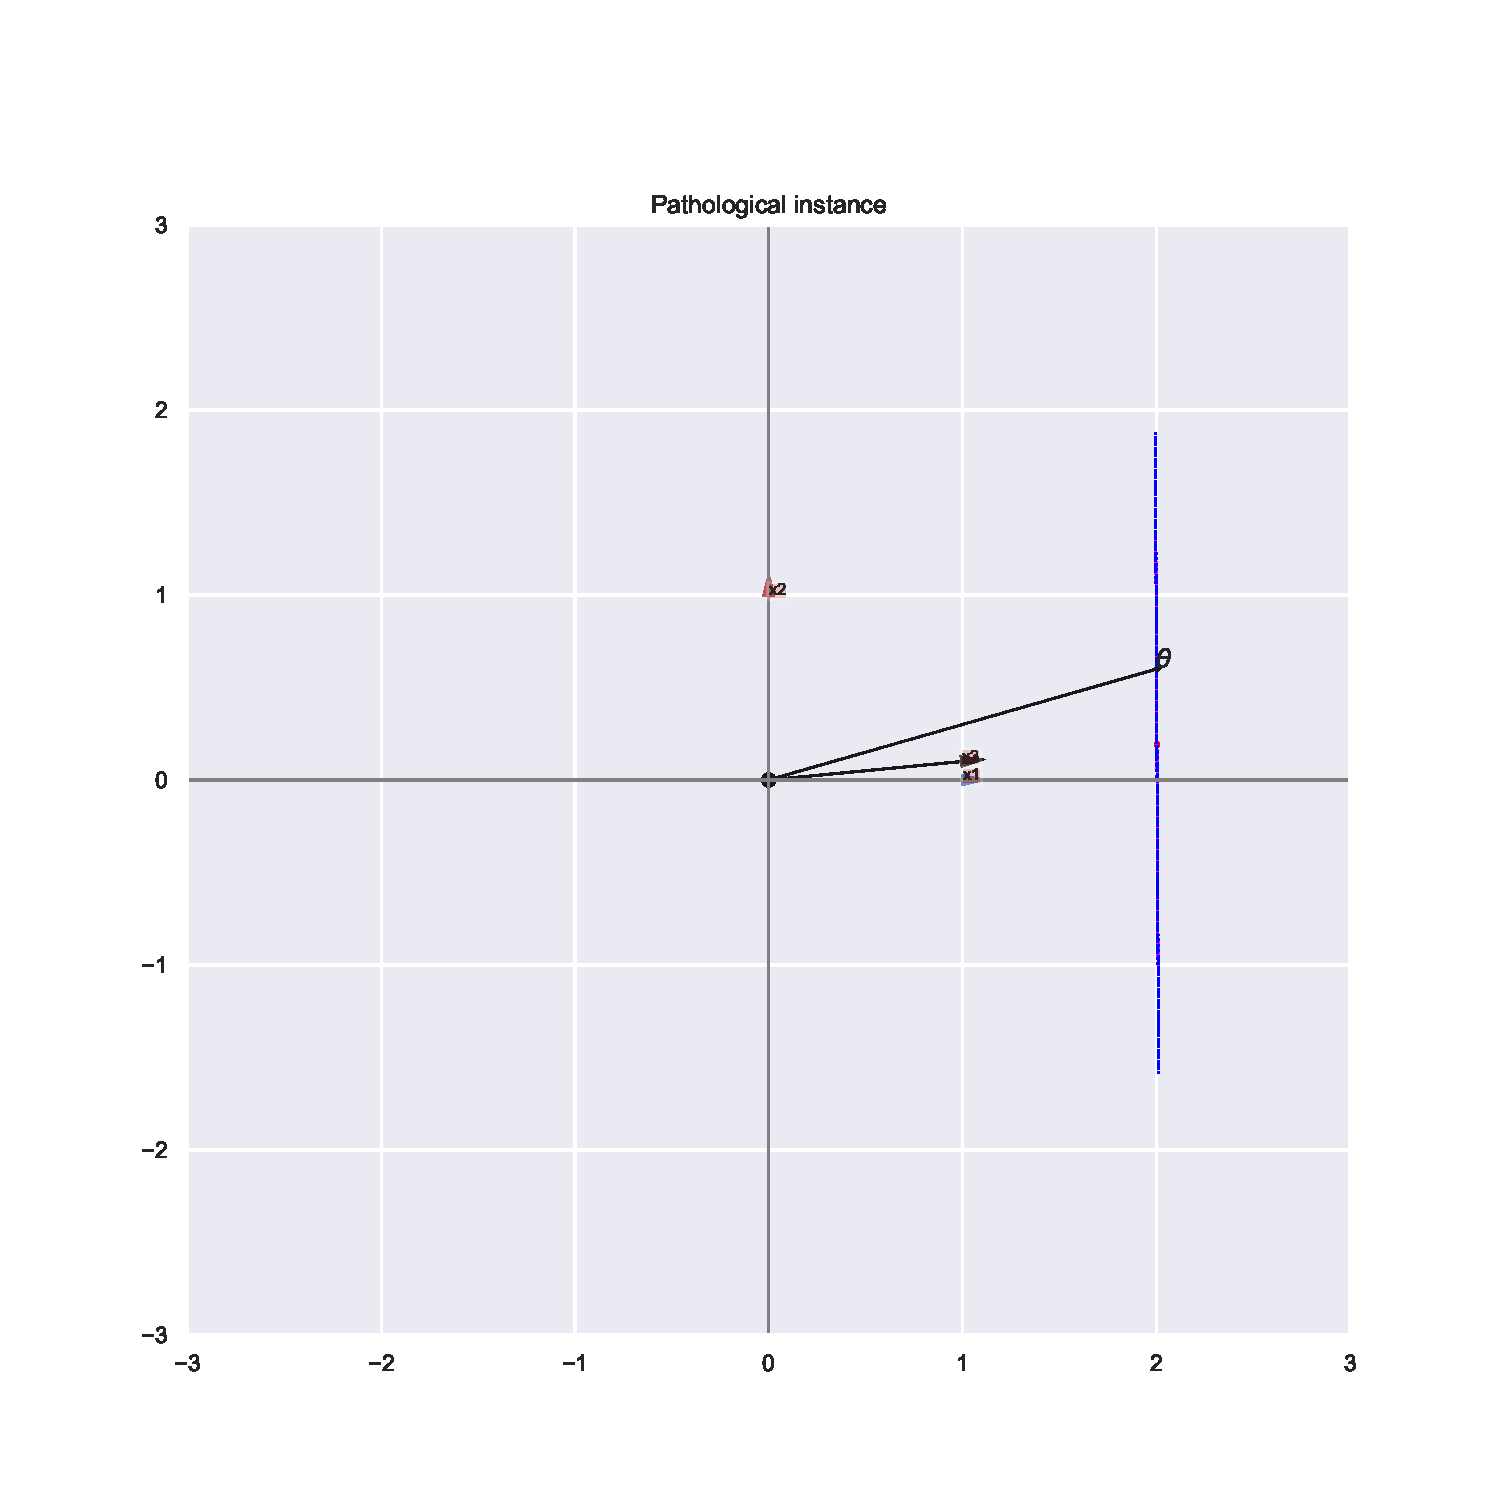
\includegraphics[width=0.55\textwidth]{Chapter4/img/instance.pdf}
    \caption{A pathological problem instance for linear best-arm identification.}
    \label{fig:instance}
\end{figure}

\subsection{A "greedy" fix of \LTCC{}}\label{sec:lgc.bayesian.fix}

A potential fix of the previous issue is the greedy version of $\LTCC$ whose pseudo-code is displayed in Algorithm~\ref{alg:lt3cg}. It is inspired by the \emph{greedy} rule already used in (a heuristic version of) \LGapE~\citep{xu2018linear}, and is motivated by the following observation: in order to learn to discriminate between some arm $I^{(1)}$ and a challenger $I^{(2)}$, it may be more informative to select another arm. More specifically, the arm from which a new pull would reduce the most the variance in the estimation of $\bx_{I^{(1)}} - \bx_{I^{(2)}}$. In a standard bandit, this is simply the least pulled arm between $I^{(1)}$ and $I^{(2)}$, but in the linear case it may be another arm!

\begin{algorithm}[ht]
\centering
\caption{Sampling rule of \LTCCG{}}
\label{alg:lt3cg}
%\footnotesize
\begin{algorithmic}[1]
    %(and the $W_n$ function for \textcolor{red}{\TCC})
   %\STATE {\bfseries Initialization:} $\forall \blambda\in\Omega, S_{\blambda}=0, F_{\blambda}=0$
   \For{$n \leftarrow 1,2,\cdots$}
        \State \text{Sample} $\btheta_1 \sim \Pi_n$
        \State $\hat{\bx}^{(1)} \leftarrow \argmax_{\bx\in\cX} \bx\transpose\btheta_1$ \text{(indexed by $I^{(1)}$)}
	        \State $I^{(2)} \leftarrow \argmin_{i\neq I^{(1)}}W_n(I^{(1)},i)$ \text{(see \eqref{def:transportation} for the definition)}\Comment{$I^{(2)} \leftarrow \hat{\bx}^{(2)}$}
		    \State \text{Evaluate arm} $\hat{\bx} \eqdef \argmin_{\bx\in\cX} \normm{\hat{\bx}^{(1)} - \hat{\bx}^{(2)}}_{(\bA_{\bX_n}+\bx\bx\transpose)^{-1}}$
	    \State \text{Update mean and variance according to \eqref{eq:update_mean} and \eqref{eq:update_variance}}
	    \State $n = n+1$
   \EndFor
\end{algorithmic}
\end{algorithm}

\subsection{\texorpdfstring{\LGapE}{} versus \texorpdfstring{\LTCCG}{}: Is one of them optimal?}\label{sec:lgc.bayesian.check}

Upon close examination, \LGapE and \LTCCG are very similar: they both rely on the computation of a leader and a challenger followed by the greedy rule to decide which arm to explore/play, and they actually use the same stopping rule (up to possible tuning of the threshold). The differences are:
\begin{itemize}
    \item how they define the challenger once the leader is chosen;
    \item how they perform exploration: \LGapE{} performs exploration in the choice of the challenger, which depends on some confidence bounds. \LTCCG{} performs exploration in the choice of the leader, which is determined by Thompson sampling.  
\end{itemize}

Table~\ref{tab:comparison} provides a more detailed comparison of the two algorithms for linear bandits. We see in particular that the stopping rule coincide up to the choice $C_n = \sqrt{2d_{n,\delta}}$.

\begin{table}[ht]
\centering
    %\hspace{-1cm}
    \resizebox{\textwidth}{!}{%
    \begin{tabular}{|c|c|c|}
    \hline 
      &  \LGapE & \LTCCG  \\
      \hline 
      Leader & $I_n^{(1)} = \argmax_{i}\bx_i\transpose\hat{\btheta}_n^{\lambda}$   &   $I_n^{(1)} = \argmax_{i} \bx_i\transpose\tilde{\btheta}_n$ \\
      & with $\hat \btheta_n^{\lambda}$ the least square estimate & with $\tilde{\btheta}_n \sim \mathcal{N}(\hat \btheta_n^\lambda,\hat{\bSigma}_n)$ \\
      \hline
        Challenger & $I_n^{(2)} = \underset{j \neq I_n^{(1)} }{\argmax} \ \left(\bx_j - \bx_{I_n^{(1)}}\right)\transpose \hat{\btheta}_n^\lambda + \normm{\bx_j - \bx_{I_n^{(1)}}}_{\hat{\bSigma}_n} C_n$    &   $I_n^{(2)} = \underset{j \neq I_n^{(1)} }{\argmin} \ddfrac{\left( \left(\bx_j - \bx_{I_n^{(1)}}\right)\transpose \hat\btheta_n^\lambda\right)^2}{2\normm{\bx_j - \bx_{I_n^{(1)}}}_{\hat{\bSigma}_n}^2} \1\left\{\bx_{I_n^{(1)}}\transpose\hat\btheta_n^\lambda \geq \bx_{j}\transpose\hat\btheta_n^\lambda\right\}$ \\
      \hline
          Stopping & $ \left(\bx_{I_n^{(2)}} - \bx_{I_n^{(1)}}\right)\transpose \hat\btheta_n^\lambda + \normm{\bx_{I_n^{(2)}} - \bx_{I_n^{(1)}}}_{\hat\bSigma_n} C_n < 0$    &  $\underset{j \neq J_n^{(1)} }{\min} \ddfrac{\left( \left(\bx_j - \bx_{J_n^{(1)}}\right)\transpose \hat\btheta_n^\lambda\right)^2}{2\normm{\bx_j - \bx_{J_n^{(1)}}}_{\hat{\bSigma}_n}^2} \1\left\{\bx_{J_n^{(1)}}\transpose\hat\btheta_n^\lambda \geq \bx_{j}\transpose\hat\btheta_n^\lambda\right\} > d_{n,\delta}$ \\
                 & $ \Leftrightarrow \ddfrac{\left(\left(\bx_{I_n^{(1)}} - \bx_{I_n^{(2)}}\right)\transpose \hat\btheta_n^\lambda\right)^2}{2\normm{\bx_{I_n^{(2)}} - \bx_{I_n^{(1)}}}_{\hat\bSigma_n}^2} > C_n^2/2$    &   $\Leftrightarrow J_n^{(1)} = \argmax_{j} \bx_j\transpose\hat{\btheta}_n^\lambda, \ \ddfrac{\left(\left(\bx_{J_n^{(1)}} - \bx_{J_n^{(2)}}\right)\transpose \hat\btheta_n^\lambda\right)^2}{2\normm{\bx_{J_n^{(2)}} - \bx_{J_n^{(1)}}}_{\hat\bSigma_n}^2} > d_{n,\delta}$ \\
          \hline
    \end{tabular}%
    }
\caption{Comparison between the two algorithms.} \label{tab:comparison}
\end{table}

\paragraph{Experiments for classical bandits.}
\LTCCG can be particularized to the classic BAI setting (that corresponds to choosing the canonical basis as contexts). In that case, the selection rule in Line 6 of Algorithm~\ref{alg:lt3cg} corresponds to choosing the least pulled arm between the two candidates. 

We investigate whether \LTCCG{} could be optimal in the classical bandit setting with some experiments. In particular, we call the derived algorithm \TCCG{}. See Fig.~\ref{fig:convergence} for a comparison against the asymptotically optimal \DT rule and the oracle. It is seemingly that \LTCCG{} is not very promising for being asymptotically optimal.

\begin{figure}[ht]
    \centering
    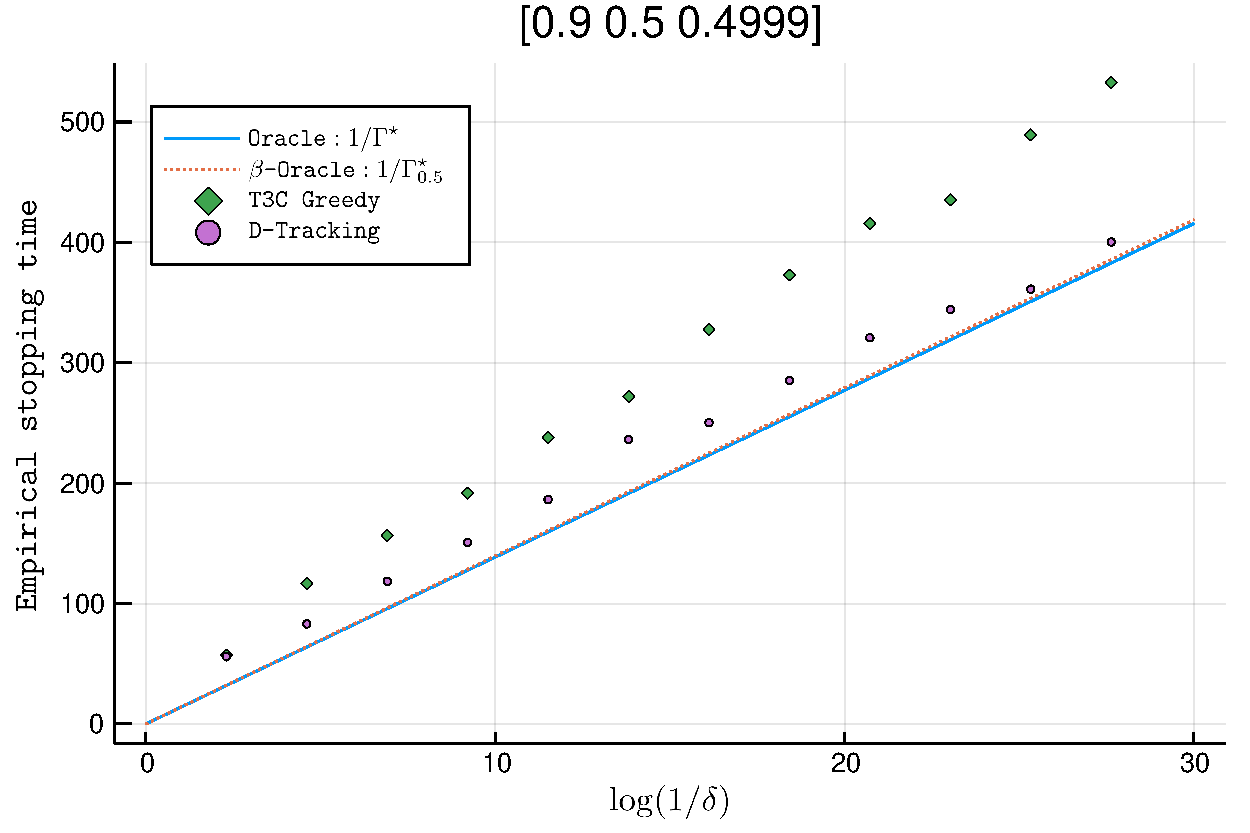
\includegraphics[width=0.33\textwidth]{Chapter4/img/res1.pdf}
    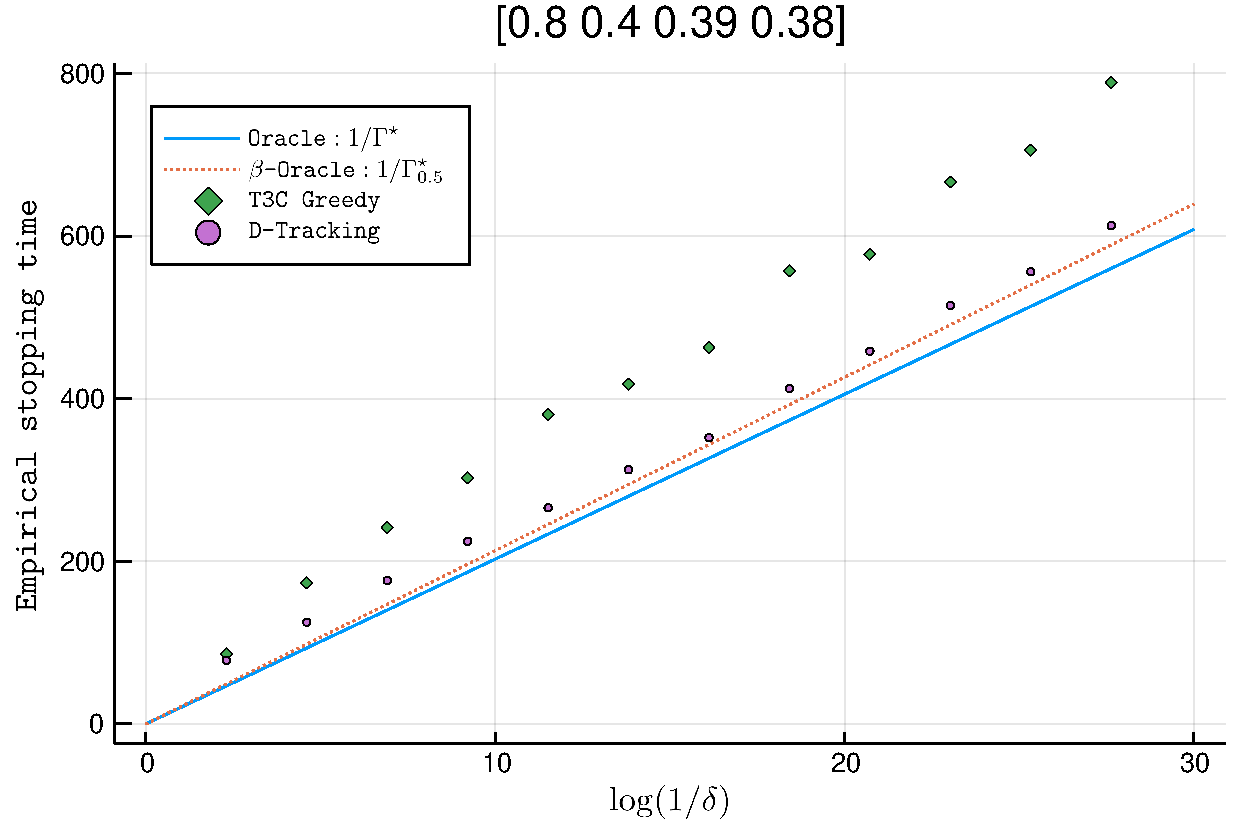
\includegraphics[width=0.33\textwidth]{Chapter4/img/res2.pdf}
    \caption{\TCCG{} versus \Track{} for different value of $\delta$.}
    \label{fig:convergence}
\end{figure}

\subsection{Empirical performance of \LTCCG{}}

\paragraph{The usual hard instance.}
We compare the performance of \LTCCG{} to \LGapE{} over the aforementioned hard instance with $d=2$, $c=2$ and two values of $\alpha$. More precisely, we report in Table~\ref{table:pulls1} the total number of pulls and also the number of pulls allocated to each arm for each of the sampling rules. The results confirm our intuition in the previous section. 

\begin{table}[ht]
\centering
\begin{tabular}{|c|c|c|}
 \hline
 & \LTCCG & \LGapE \\
 \hline
 \textbf{$\bx_1=(1,0)\transpose$} & $1783.1$ & $5844.4$ \\
 \hline
 \textbf{$\bx_2=(0,1)\transpose$} & $357009.0$ & $1169260.5$ \\
 \hline
 \textbf{$\bx_3=(\cos(0.01),\sin(0.01)\transpose)$} & $1.0$ & $1.0$ \\
 \hline
 \textbf{Total} & $\textbf{358793.1}$ & $1175105.9$ \\
 \hline
\end{tabular}
\caption{Average number of pulls of each arm ($d=2, \delta=0.1$).}
\label{table:pulls1}
\end{table}

\begin{table}[ht]
\centering
\begin{tabular}{|c|c|c|c|}
 \hline
 & \LTCC ($\beta=1/2$) & \LTCCG & \LGapE \\
 \hline
 \textbf{$\bx_1=(1,0)\transpose$} & $131.3$ & $24.9$ & $26.3$ \\
 \hline
 \textbf{$\bx_2=(0,1)\transpose$} & $3.3$ & $60.8$ & $63.4$ \\
 \hline
 \textbf{$\bx_3=(\cos(\pi/4),\sin(\pi/4)\transpose)$} & $133.4$ & $1.0$ & $1.0$ \\
 \hline
 \textbf{Total} & $268.0$ & $\textbf{86.7}$ & $89.7$ \\
 \hline
\end{tabular}
\caption{Average number of pulls of each arm ($d=2, \delta=0.1$).}
\label{table:pulls2}
\end{table}

\paragraph{Arms with mild gaps.}
We can also provide more experimental illustrations on different types of problem.

We construct a set of $K$ arms proposed by~\cite{fiez2019transductive}:
\[
    \bx_1=(1,0)\transpose, \bx_2=(\cos(3\pi/4),\sin(3\pi/4))\transpose\,,
\]
and for $k = 3,\ldots,K$, 
\[
    \bx_k=(\sin(\pi/4+\phi_k),\cos(\pi/4+\phi_k))\transpose
\]
where $\phi_i\sim\cN(0,0.09)$. We fix the true regression parameter $\theta$ to be $\be_1$. This set of arms has some nice properties, that $\bx_1$ is the optimal arm, and $\bx_2$ is the arm that gives more information on identifying the best arm. We first report results with a moderate $K=6$ as an example where the generated expected means are $[1.0, -0.71, 0.84, -0.95, 0.93, 0.99]$.

\begin{table*}[ht]
\centering
\def\arraystretch{1.2}
\begin{tabular}{|c|c|c|c|}
 \hline
 & \LTCC & \LTCCG & \LGapE \\
 \hline
 \textbf{$\bx_1=(1,0)\transpose$} & $170872.19$ & $1.06$ & $1.13$ \\
 \hline
 \textbf{$\bx_2=(\cos(3\pi/4),\sin(3\pi/4))\transpose$} & $1.25$ & $1.0$ & $1.0$ \\
 \hline
 \textbf{$\bx_3=(\sin(\pi/4+\phi_3),\cos(\pi/4+\phi_3))\transpose$} & $92.18$ & $28693.26$ & $120657.6$ \\
 \hline
 \textbf{$\bx_4=(\sin(\pi/4+\phi_4),\cos(\pi/4+\phi_4))\transpose$} & $1.12$ & $26197.03$ & $110157.63$ \\
 \hline
 \textbf{$\bx_5=(\sin(\pi/4+\phi_5),\cos(\pi/4+\phi_5))\transpose$} & $77.04$ & $1.0$ & $1.0$ \\
 \hline
 \textbf{$\bx_6=(\sin(\pi/4+\phi_6),\cos(\pi/4+\phi_6))\transpose$} & $170892.82$ & $1.36$ & $1.83$ \\
 \hline
 \textbf{Total} & $341936.6$ & $\textbf{54894.71}$ & $230820.19$ \\
 \hline
\end{tabular}
\caption{average number of pulls of each arm ($d=2, \delta=0.1$).}
\label{table:pulls3}
\end{table*}

\paragraph{Impact of the dimension.}
We also compare the impact of the dimension $d$ over the performance of our sampling rule and $\LGapE$. We run experiments on the same instance with a value of the angle set to $\alpha=0.1$. This time we let the dimension $d$ varying from 2 to 6. \LTCC{} is always better and the performance gap increases with the dimension. Thus, our algorithm seems to be more robust to the dimension.

\begin{figure}[ht]
    \centering
    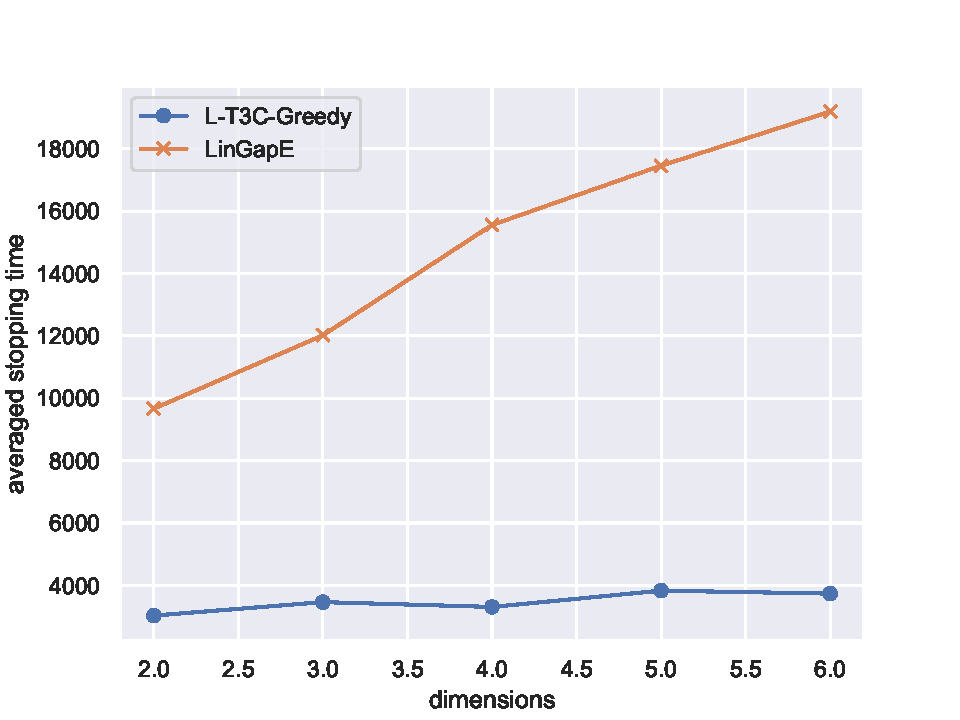
\includegraphics[width=0.5\textwidth]{Chapter4/img/dims.pdf}
    \caption{Comparison of the sample complexity of \LTCCG{} and \LGapE{} on the pathological instance in $\R^d$ for different values of $d$.}
    \label{fig:dims}
\end{figure}

\paragraph{Rank-1 multivariate normal distribution sampling.}
A technical point for the experiments in this section is to sample from a multivariate normal distribution (e.g. for \LTCC{}). We can proceed by the following.

Indeed, a random Gaussian vector 
\[
    \bX = (X_1, X_2, \ldots, X_d)\transpose
\] 
of mean vector $\bar{\bmu}$ and covariance matrix $\bSigma$ can be formally defined as following,
\[
    \bX \sim \cN(\bar{\bmu}, \bSigma) \iff \exists \bar{\bmu}\in\mathbb{R}^d,\bA\in\mathbb{R}^{d\times d'} \ \text{s.t.} \ \bX = \bA \mathbf{Z} + \bar{\bmu},
\]
for $Z_i \sim\ \mathcal{N}(0, 1)$ i.i.d. with $i\in\{1,\ldots,d'\}$, and here $\bSigma = \bA\bA\transpose$.

To draw a sample from a multivariate normal distribution, according to the previous definition, one can first find any real matrix $\bA$ such that $\bA\bA\transpose = \bSigma$. Then draw a vector $\bZ$ whose components independently follow standard normal distribution. Finally $\bX = \bA \mathbf{Z} + \bar{\bmu}$ forms a valid sample. The main issue is thus how to find an appropriate matrix $\bA$.

In this section, we need to sample from $\cN(\hat{\btheta}^\lambda_n,\hat{\bSigma}_n)$, where the covariance matrix $\hat{\bSigma}_n$ is a positive-definite matrix. A usual way is to apply the Cholesky decomposition, which is computationally inefficient if it were to be applied at each time step. Fortunately, we can apply rank-1 Cholesky decomposition in our case.  

%We, however, notice that $\bA = (\hat{\bSigma}_n)^{1/2}=\sigma(\bB^{\lambda}_n)^{-1/2}$ is also a valid candidate, and is thus can be also updated iteratively using a similar formula to the Sherman-Morrison formula.

%More precisely, we have
%\begin{align*}
%    \forall t\geq 0, \quad (\bB^{\lambda}_{t+1})^{-\frac{1}{2}} = (\bB^{\lambda}_t)^{-\frac{1}{2}} - \ddfrac{\left(1-\sqrt{1-\frac{\normm{\hat{\bx}_{t+1}}_{(\bB^{\lambda}_t)^{-1}}^2}{1+\normm{\hat{\bx}_{t+1}}_{(\bB^{\lambda}_t)^{-1}}^2}}\right)}{\normm{\hat{\bx}_{t+1}}_{(\bB^{\lambda}_t)^{-1}}^2} (\bB^{\lambda}_t)^{-\frac{1}{2}}\hat{\bx}_{t+1}\hat{\bx}_{t+1}\transpose(\bB^{\lambda}_t)^{-\frac{1}{2}}.
%\end{align*}

% \subsection{Technical tools}

% \subsection{Tail bounds}
% Following are the classic Gaussian tail bound inequalities written in our linear context (see e.g.~\citealt{qin2017ttei} for detailed proofs).

% \begin{lemma}\label{lemma:tail_upper}
% For any $i,j\in\{1,\ldots,K\}$, if $\bx_i\transpose\hat{\btheta}^\lambda_n<\bx_j\transpose\hat{\btheta}^\lambda_n$,
% \begin{align}
%     \Pi_n\left[\bx_i\transpose\btheta>\bx_j\transpose\btheta\right] &\leq \frac{1}{2} \expp{-\frac{\left(\bx_j\transpose\hat{\btheta}^\lambda_n-\bx_i\transpose\hat{\btheta}^\lambda_n \right)^2}{2\normm{\bx_i-\bx_j}_{\hat{\bSigma}_n}^2}}.
% \end{align}
% \end{lemma}

% \begin{lemma}\label{lemma:tail_lower}
% For any $i,j\in\{1,\ldots,K\}$, if $\bx_i\transpose\hat{\btheta}^\lambda_n<\bx_j\transpose\hat{\btheta}^\lambda_n$,
% \begin{align}
%     \Pi_n\left[\bx_i\transpose\btheta>\bx_j\transpose\btheta\right] &\geq \frac{1}{\sqrt{2\pi}} \expp{-\frac{\left(\bx_j\transpose\hat{\btheta}^\lambda_n-\bx_i\transpose\hat{\btheta}^\lambda_n +\normm{\bx_i-\bx_j}_{\hat{\bSigma}_n}\right)^2}{2\normm{\bx_i-\bx_j}_{\hat{\bSigma}_n}^2}}.
% \end{align}
% \end{lemma}


%!TEX root = ../Chapter4.tex
\section{Other Saddle-Point Approaches}\label{sec:lgc.sp}

Methods based on approaching the saddle point of the lower bound look promising, one concern about \LG{} (or \LGC{}) could be its computational complexity though. In BAI, the one step complexity of \LG{} is dominated by the computation of the best response for nature, which requires a full matrix inversion. Alternatives that involve rank-1 updates should be considered.

We end this chapter by some more discussions on other possible saddle-point methods.

\subsection{Linear \texorpdfstring{\Track{}}{}}

Although never formally proved, the linear version of \Track seems to be another plausible candidate of being asymptotically optimal provided that a numerical solver for computing the optimal weights exists. Fortunately, the Algorithm~\ref{alg:fw_ab} proposed in Section~\ref{sec:lgc.complexity.complexity} seems to be one. 

\Track remains unchanged in the linear case, since it only cares about tracking the optimal weights. We hereby recall that the \CT rule consists of playing
\[
    \hat\bx \in \argmax_{i\in[K]} \sum_{t=0}^n \omega_i^{\epsilon_t}(\hat\bmu_t)-T_{t,i}\,,
\]
where $\bomega^\epsilon$ is a $L^\infty$ projection of $\bomega^\star$ onto the simplex $\Sigma_K^\epsilon \eqdef \{\bomega\in [\epsilon,1]^K : \sum_{i=1}^K \omega_i = 1\}$. The draw back of \Track is that we need to compute a plug-in estimate of the optimal weights at each stage, which is computationally unfavorable.

\subsection{Saddle-point Frank-Wolfe}
On the other hand, the Frank-Wolfe heuristic in Algorithm~\ref{alg:fw_ab} is an efficient rank-1 solver. It is thus natural to investigate if it can be incorporated into existing algorithms. 

In particular, we can propose two new algorithms by adding the solver on top of \LGapE (resp. \LTCC) that we call \SLGapE (resp. \SLTCC), as shown in Algorithm~\ref{alg:slgape} (resp. Algorithm~\ref{alg:slt3c}). We define a so called \emph{active transductive set} as
\begin{align}\label{def:active_transductive}
    \hat\cY(\bx,\btheta) \eqdef \left\{ \frac{(\bx- \bx')}{\left|(\bx-\bx')\transpose\btheta\right|}: \bx'\in\cX/\big\{\bx\big\}  \right\}\,.
\end{align}

\begin{algorithm}[ht]
\centering
\caption{Algorithm of \SLGapE{}}
\label{alg:slgape}
%\footnotesize
\begin{algorithmic}[1]
    \State {\bfseries Input:} $\delta$
    \State {\bfseries Initialize:} $\mathbf{\tLambda} \leftarrow{} I_d, \mathbf{\Lambda}\leftarrow{} I_d$

   \For{$n \leftarrow 1,2,\cdots$}
        \State $\mathbf{\hat{\bx}}\in\argmax_{\bx\in\cX}  \norm{\bx}_{\mathbf{\Lambda}^{-1} \mathbf{\tLambda} \mathbf{\Lambda}^{-1} }^2$
        \State $\hat{\bx}^{(1)} \leftarrow \argmax_{\bx\in\cX} \bx\transpose\hat\btheta^{\lambda}_n$
        \State $\hat{\bx}^{(2)} \leftarrow \argmax_{\bx\neq\hat{\bx}^{(1)}} (\bx-\hat{\bx}^{(1)})\transpose\hat\btheta^{\lambda}_n + \sqrt{2\beta(n,\delta)}\normm{\hat{\bx}^{(1)}-\bx}_{\bLambda^{-1}}$
        \State $B_n \leftarrow \max_{\bx\neq\hat{\bx}^{(1)}} (\bx-\hat{\bx}^{(1)})\transpose\hat\btheta^{\lambda}_n + \sqrt{2\beta(n,\delta)}\normm{\hat{\bx}^{(1)}-\bx}_{\bLambda^{-1}}$
        \If{$B_n \leq 0$}
            \State \Return $\hat{\bx}^{(1)}$
        \EndIf
        \State $\hat\by \leftarrow{} \dfrac{(\hat{\bx}^{(1)}- \hat{\bx}^{(2)})}{(\hat{\bx}^{(1)}-\hat{\bx}^{(2)})\transpose\btheta}$
        \State $\bLambda\leftarrow{} \mathbf{\Lambda}+ \mathbf{\hat\bx}\mathbf{\hat\bx}\transpose$
		\State $\mathbf{\tLambda} \leftarrow{} \mathbf{\tLambda} + \mathbf{\hat\by}\mathbf{\hat\by}\transpose$
		\State \text{Evaluate arm} $\hat{\bx}$
	    \State \text{Update mean and variance according to \eqref{eq:update_mean} and \eqref{eq:update_variance}}
	    \State $n = n+1$
   \EndFor
\end{algorithmic}
\end{algorithm}

\begin{algorithm}[ht]
\centering
\caption{Sampling rule of \SLTCC{}}
\label{alg:slt3c}
%\footnotesize
\begin{algorithmic}[1]
   \State {\bfseries Initialize:} $\mathbf{\tLambda} \leftarrow{} I_d, \mathbf{\Lambda}\leftarrow{} I_d$

   \For{$n \leftarrow 1,2,\cdots$}
        \State \text{Sample} $\btheta \sim \Pi_n$
        \State $\mathbf{\hat{\bx}}\in\argmax_{\bx\in\cX}  \norm{\bx}_{\mathbf{\Lambda}^{-1} \mathbf{\tLambda} \mathbf{\Lambda}^{-1} }^2$
        \State $\mathbf{\hat{\by}}\in\argmax_{\by\in\hat\cY(\hat\bx,\btheta)}\normm{\by}^2_{\mathbf{\Lambda}^{-1}}$
        \State $\mathbf{\Lambda}\leftarrow{} \mathbf{\Lambda}+ \mathbf{\hat\bx}\mathbf{\hat\bx}\transpose$
		\State $\mathbf{\tLambda} \leftarrow{} \mathbf{\tLambda} + \mathbf{\hat\by}\mathbf{\hat\by}\transpose$
		\State \text{Evaluate arm} $\hat{\bx}$
	    \State \text{Update mean and variance according to \eqref{eq:update_mean} and \eqref{eq:update_variance}}
	    \State $n = n+1$
   \EndFor
\end{algorithmic}
\end{algorithm}

\subsection{Experimental illustrations}

We compare our saddle-point-based algorithms against \LGapE{}. To make a fair comparison, we use always the same exploration rate for all the stopping rules. Indeed the stopping rules are equivalent if they keep the same exploration rate as argued in Appendix~\ref{app:lgc.stopping}. We use the previous hard instance with $c=1$, the results are reported as box plots of average stopping time in Figure~\ref{fig:exp1}.

It seems that they can achieve the same level of empirical performance as \LGapE{}, their theoretical behaviour thus turns out to be an interesting research direction for the future.

\begin{figure}[ht]
    \centering
    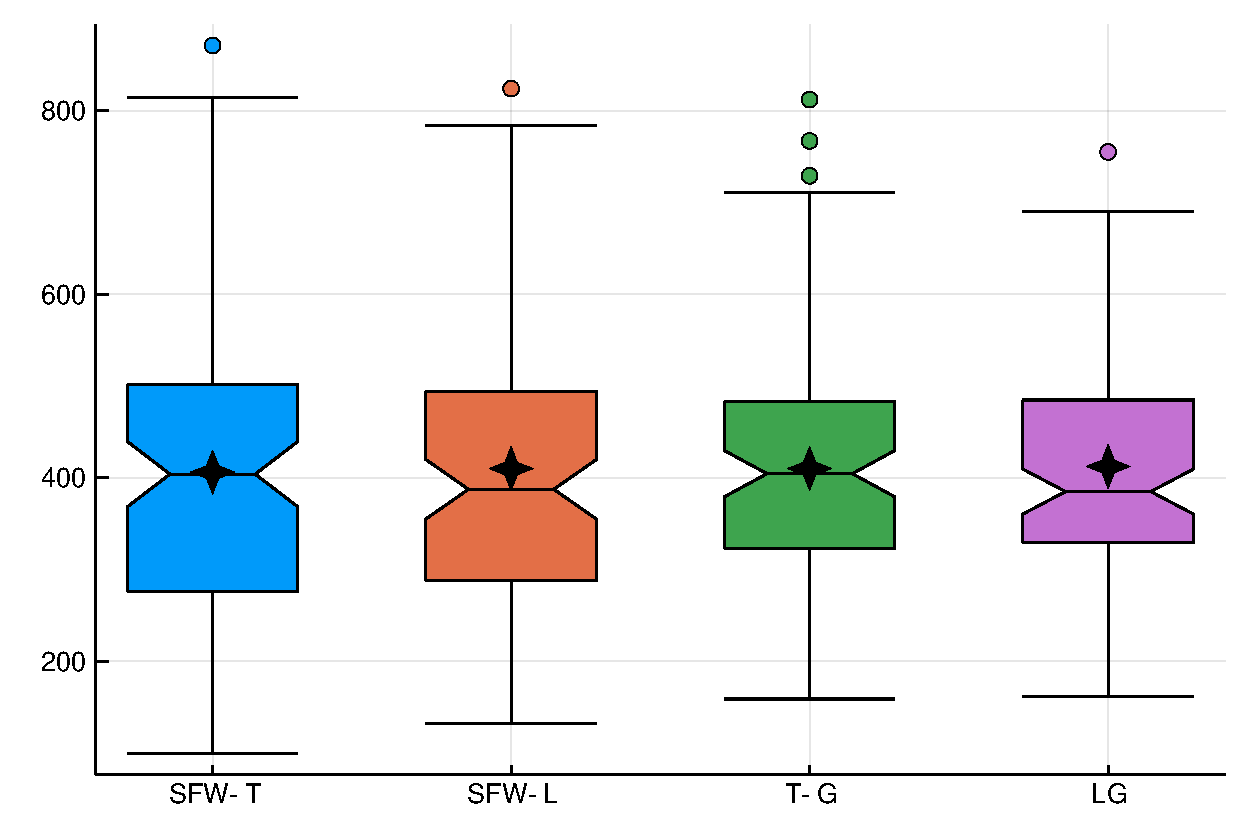
\includegraphics[width=0.33\textwidth]{Chapter4/img/exp_sin_-0000001}
    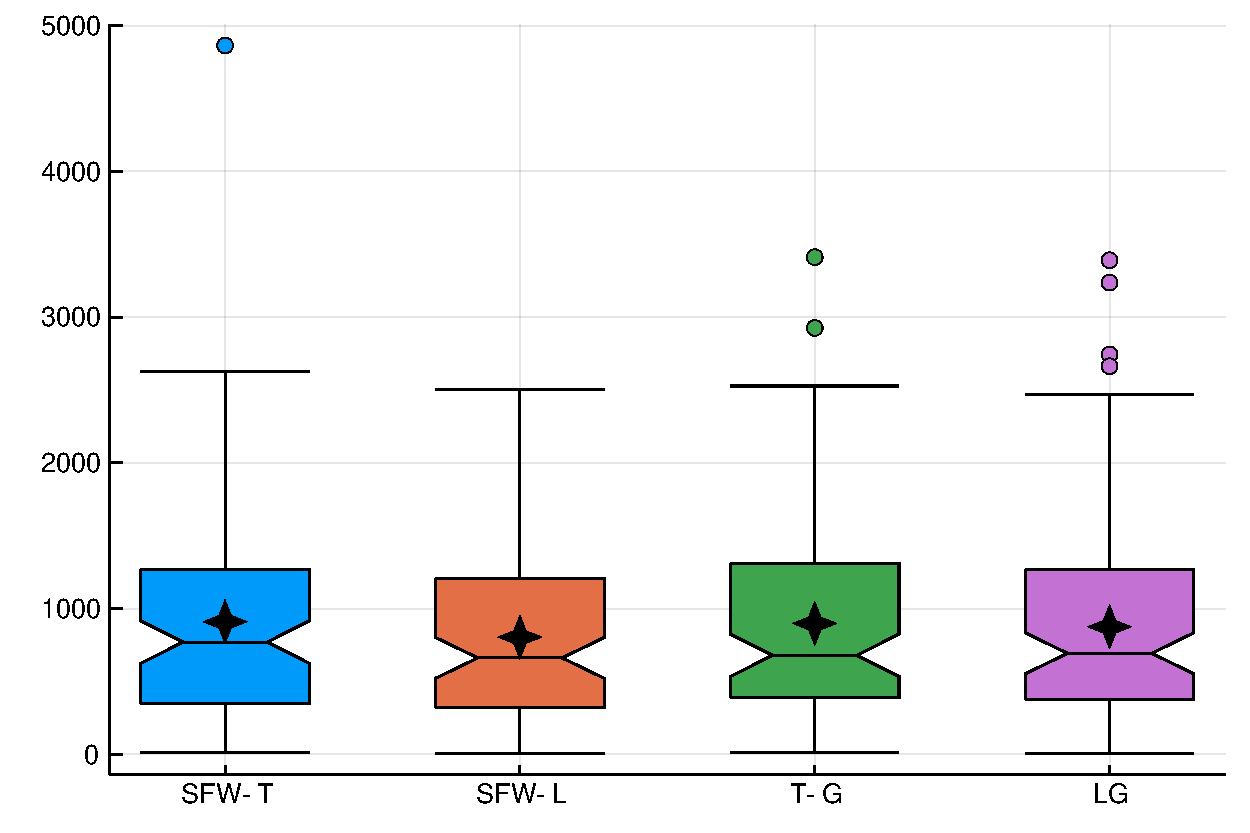
\includegraphics[width=0.33\textwidth]{Chapter4/img/exp_sin_-1}
    \caption{Average stopping time (Left: $d=2,\alpha=\pi/4,\delta=0.0000001$, Right: $d=2,\alpha=0.1,\delta=0.1$), with SFW-T = \SLTCC{}, SFW-L = \SLGapE{}, T-G = \LTCC{}, LG = \LGapE{}.}
    \label{fig:exp1}
\end{figure}


%!TEX root = ../Chapter4.tex
\section{A Gamified Algorithm}\label{sec:lgc.game}

The first attempt using Bayesian machinery does not end up with a satisfying output. In this section, we turn our thoughts to another idea and take inspiration from the \emph{zero-sum game} (see e.g.~\citealt{degenne2019pure}). We describe \LG{}, detailed in Algorithm~\ref{alg:lg}. As noted in the seminal work of \citet{chernoff1959}, the complexity $\Tstar(\btheta)^{-1}$ is the value of a fictitious zero-sum game between the learner choosing an optimal proportion of allocation of pulls $\bomega$ and a second player, the nature, that tries to fool the agent by responding with the most confusing alternative $\btheta'$ leading to an incorrect answer. \LG{} is an asymptotically optimal algorithm for linear bandits BAI. Note that the present algorithm is asymptotically optimal for the general pure exploration game, which is however not the main focus of this thesis. Lecturers can refer to~\cite{degenne2020game} for more details.

In this section, we make the following extra assumption.
\begin{assumption}\label{ass:lgc.bounded_parameter}
\begin{leftbar}[assumptionbar]
We assume that $\exists M>0$, s.t. $\forall \btheta\in\Theta$, $\normm{\btheta} \leq M$, where $\normm{\btheta}$ denotes the Euclidean norm of the vector $\btheta$. 
\end{leftbar}
\end{assumption}

%The full analysis of the algorithm is omitted as well as a convexified version \LGC{} -- also asymptotically optimal itself -- as they are not the main focus of this thesis. Lecturers can refer to~\cite{degenne2020game} for the complete proofs.


% , i.e for $i\in\cI$ and $w\in\interior{\Sigma_A}$ in the interior of the probability simplex of dimension $A-1$, find $\lambda^i$ such that
% \[
% \lambda^i \in \argmin_{\lambda\neg i}\normm{\theta - \lambda }_{V_{w}}\,.
% \]


%Note that in the proof of Theorem~\ref{thm:sample_complexity} we only use two times the boundedness assumption, first in the definition of the threshold $\beta(t,\delta)$ (see Theorem~\ref{th:confidence_beta}) to handle the bias induced by the regularization. Second, since the regret of AdaHedge is proportional to the maximum of the upper confidence bounds $U_s^{i,a}$, we need to ensure that they are bounded.

% And there exists pathological pure exploration problems where even the quantity uppper bounded by $U_s^{i,a}$, namely $\normm{\theta-\lambda}_{aa^\top}^2$ where $\lambda\in\argmin_{\lambda'\in\neg i}\normm{\theta -\lambda}$ is unbounded\todo{I don't understand what this means.}. See for example Appendix~G.3 by \citet{menard2019lma}.

\subsection{Notations}

In this section, besides the usual learner, we include an extra fictive player -- the nature -- and we thus introduce some specific notation of counts for this section.

At each round $n$ the algorithm to be presented will play an arm $\hbx_n$ and choose (fictitiously) an answer $i_n\in\cI$. We denote by $N_n^{\bx,i} \eqdef\sum_{t=1}^n \ind_{\{(\hbx_n,i_n)=(\bx,i)\}}$ the number of times the pair $(\bx,i)\in\cX\times\cI$ is chosen up to and including time $n$, and by $N_n^\bx =\sum_{i\in\cI} N_n^{\bx,i}$ and $N_n^i =\sum_{\bx\in\cX} N_n^{\bx,i}$ the partial sums. The vectors of counts at time $n$ is denoted by $\bN_n \eqdef (N_n^\bx)_{\bx\in\cX}$
and when it is clear from the context we will also denote by $\bN_n^{\bx} = (N_n^{\bx,i})_{i\in\cI}$ and $\bN_n^i = (N_n^{\bx,i})_{\bx\in\cX}$ the vectors of partial counts. Remind that in the case of BAI, $\cX=\cI$.

%\paragraph{Regularized least square estimator.} We fix a regularization parameter $\eta > 0$. The regularized least square estimator for the parameter $\theta\in \mathcal M$ at time $t$ is
%\[
%\htheta_{t} = (V_{N_t} + \eta I_d)^{-1} \sum_{s=1}^t Y_s a_s\,,
%\]
%where $I_d$ is the identity matrix. By convention $\htheta_0 = 0$.


\subsection{The \LG{} algorithm}

The pseudo-code of \LG{} is provided in Algorithm~\ref{alg:lg}. We interpret each component of the algorithm by next.

\begin{algorithm}[ht]
\centering
\caption{Algorithm of \LG{}}
\label{alg:lg}
\begin{algorithmic}[1]
    \State {\bfseries Input:} Learners for each answer $(\cL^i_\bomega)_{i\in\cI}$, threshold $d$
    \For{n = 1 \ldots}
        \State \textit{// Stopping rule}
        \If{{$\max_{i\in\cI}\inf_{\btheta'\in\neg i} \frac{1}{2}\normm{\hbtheta_{n-1}^\lambda-\btheta'}^2_{\bLambda_{\bN_{n-1}}}\geq d_{n-1,\delta}$}}
            \State \text{Stop} 
            \State {\bfseries Return} $J_n = \Istar(\hbtheta_{n-1}^\lambda)$
        \EndIf
        \State \textit{// Empirical best guess}
        \State $i_n = \Istar(\hbtheta_{n-1}^\lambda)$
        \State \textit{// Learner plays first}
        \State \text{Get} $\bomega_n$ \text{from} $\cL^{i_n}_\bomega$
        \State \text{Update} $\bW_n=\bW_{n-1}+\bomega_n$
        \State \textit{// Best response of the nature}
        \State $\btheta_n^{i_n} \in \argmin_{\btheta'\in\neg i_n}\normm{\hbtheta_{n-1}^\lambda-\btheta'}^2_{\bLambda_{\bomega_n}}$
        \State \textit{// Feed optimistic gains}
        \State \text{Feed learner} $\cL_\bomega^{i_n}$ \texttt{with} $g_{n}(\bomega) = \sum_{\bx\in\cX}\omega_\bx U_n^{\bx,i_n}/2$
        \State \textit{// Track the weights}
        \State \text{Pull} $\hbx_n \in \argmin_{\bx\in \cX} N_{n-1}^{\bx} - W_{n,\bx}$
   \EndFor
\end{algorithmic}
\end{algorithm}

% \begin{algorithm}[tb]
% \centering
% \caption{\LGC}
% \label{alg:lgc}
% \begin{algorithmic}[1]
%     \State {\bfseries Input:} Agent learner $\cL_{\tw}$, threshold $\beta(\cdot,\delta)$
%     \For{t = 1 \ldots}
%         \State \textit{// Stopping rule}
%         \If{ {\small $\max_{i\in \cI} \inf_{\lambda\in\neg i} \frac{1}{2}\normm{\htheta_{t-1}-\lambda}^2_{V_{N_{t-1}}}\geq \beta(t-1,\delta)$}}
%             \State {\bfseries stop} and {\bfseries return} $\hi = \istar(\hat{\theta}_{t-1})$. 
%         \EndIf
%         \State \textit{// Agent plays first}
%         \State \texttt{get} $\tw_{t}$ \texttt{from} $\cL_{\tw}$ 
%         \State \texttt{update} $\tW_{t}=\tW_{t-1}+\tw_{t}$
%         \State \textit{// Best response for the nature}
%         \State $\forall i\in\cI$, $\tlambda^i_{t} \in \argmin_{\lambda\in\neg i}\normm{\htheta_{t-1}-\lambda}^2_{V_{\tw^i_{t}}}$
%         \State \textit{// Feed optimistic gains}
%         \State \texttt{feed learner} $\cL_{\tw}$ \texttt{with} {$g_{t}(\tw) =\sum_{(a,i)\in\cA\times\cI} \tw^{a,i} U_t^{a,i}/2$}
%         \State \textit{// Track the weights}
%         \State \texttt{pull} $(a_{t},i_{t})\in \argmin_{(a,i)\in \mathcal A \times \mathcal I} N_{t-1}^{a,i} - \tW_{t}^{a,i}$
%     \EndFor
% \end{algorithmic}
% \end{algorithm}

\paragraph{Stopping rule and decision rule.}
We follow the same stopping rule and decision rule of Section~\ref{sec:lgc.bayesian}\footnote{It is easy to check that~\eqref{eq:lgc.lg_stopping} and~\eqref{eq:lgc.lg_decision}) are equivalent to~\eqref{eq:lgc.bayesian_stopping} and~\eqref{eq:lgc.bayesian_decision} respectively.}: \LG{} stops if a generalized likelihood ratio exceeds a threshold $d_{n,\delta}$. With the notation of this section, the stopping time can be written as
\begin{align}\label{eq:lgc.lg_stopping}
    \max_{i\in \cI} \inf_{\btheta' \in \neg i}\frac{1}{2}\Vert \hbtheta_n^\lambda - \btheta' \Vert^2_{\bLambda_{\bN_n}} > d_{n,\delta}\,,
\end{align}
and the decision rule is 
\begin{align}\label{eq:lgc.lg_decision}
    J_n = \argmax_{i\in \cI} \inf_{\btheta' \in \neg i}\Vert \hbtheta_n^\lambda - \btheta' \Vert^2_{\bLambda_{\bN_n}}/2\,.
\end{align}

Similarly to \TCC{}/\TTTS{} of Chapter~\ref{CHAP:T3C}, these stopping and decision rules ensure that the \LG{} is $\delta$-correct regardless of the sampling rule used, see lemma below\footnote{The fact that $\tau_\delta <+\infty$ is a consequence of our analysis, see Appendix~\ref{app:lgc.proof}.} proved in Appendix~\ref{app:lgc.lemmas}.

\begin{lemma}\label{lemma:lgc.pac}
\begin{leftbar}[lemmabar]
Regardless of the sampling rule, the stopping rule~\eqref{eq:lgc.lg_stopping} with the threshold
\begin{equation} \label{eq:def_beta}
    d_{n,\delta} =\left( \sqrt{\log\left( \frac{1}{\delta}\right)+\frac{d}{2}\log\left(1+\frac{n L^2}{\lambda d} \right)} +\sqrt{\frac{\lambda}{2}}M\right)^2\,,
\end{equation}
satisfy
\[
    \PPt{\big(\tau_{\delta} < \infty \wedge J_\tau \neq \Istar(\btheta)\big)} \leq \delta\,.
\]
\end{leftbar}
\end{lemma}
% This stopping and decision rules ensures that the algorithm is $\delta$-correct regardless of the sampling rule used (see \citealt{garivier2016tracknstop} for a proof), hence the following theorem is immediate.
% \begin{theorem}
% Algorithms~\ref{alg:lg} and~\ref{alg:lgc} are $\delta$-correct.
% \end{theorem}
Our contribution is a sampling rule that minimizes the sample complexity when combined with these stopping and decision rules.
We now explain our sampling strategy to ensure that the stopping threshold is reached as soon as possible.

\paragraph{Saddle-point computation.}
Suppose in this paragraph, for simplicity, that the regression parameter $\btheta$ is known to the learner. By the definition of stopping rule and generalized likelihood ratio, as long as the algorithm does not stop, we have
\begin{align*}
    d_{n,\delta} \ge \inf_{\btheta'\in \neg \Istar(\btheta)} \sum_{\bx\in \cX} N_n^\bx \Vert \btheta - \btheta' \Vert^2_{\bx\bx\transpose}/2\,.
\end{align*}
Now, let $\bomega^\star(\btheta)$ be the optimal pulling proportions given $\btheta$. If we manage to have $\bN_n \approx n\bomega^\star(\btheta)$, then it follows $d_{n,\delta} \ge n T^\star(\btheta)^{-1}$ and, solving that equation would lead to the asymptotic optimality.

% Since there is only one correct answer, the parameter $\btheta$ belongs to all sets $\neg i$ for $i\neq \Istar(\btheta)$. Hence
% \begin{align*}
% &\inf_{\lambda\in \neg i^\star(\theta)}\frac{1}{2} \sum_{a\in \cA} N_t^a \Vert \theta - \lambda \Vert^2_{a a^\top}
% \\&\geq \inf_{\tlambda_t\in \prod_i (\neg i)}\frac{1}{2}\sum_{(a,i)\in \cA\times\cI}\!\!\!\!\! N_t^{a,i} \Vert \theta - \tlambda^i \Vert^2_{a a^\top}.
% \end{align*} Introducing the sum removes the dependence in the unknown $i^*(\theta)$. \LGC then uses an agent playing weights w in $\Sigma_{\cA\cI}$. 

At each time step, \LG{} produces a guess $i_n$ for $\Istar(\btheta)$ and its analysis involves proving that the guess is wrong only finitely-many times in expectation.

The sampling rule implements a lower-bound game between a learner, playing at each stage $n$ a pull-proportion/weight vector $\bomega_n$ in the probability simplex $\Sigma_K$, and nature, who computes at each stage a response $\btheta_n \in \neg i_n$. We additionally ensure that $N_n^\bx \approx \sum_{t=1}^n \omega_{t,\bx}$, where $\omega_{n,\bx}$ denotes the weight of $\bx$ at stage $n$. The goal of the sampling rule is to ensure a $\epsilon$-approximation of the saddle point of the lower-bound game.

% Suppose that the sampling rule is such that at stage $t$, a $\varepsilon_t$-approximate saddle point is reached for the lower-bound game, see Lemma~\ref{lem:sion_convexify}. That is,
% \begin{align*}
% &\inf_{\tlambda \in \prod_{i}(\neg i)} \sum_{s=1}^t \sum_{(a,i)\in \cA\times\cI} \tw_s^{i,a} \Vert \theta - \tlambda^i \Vert^2_{a a^\top}/2 +\varepsilon_t
% \\
% &\ge \sum_{s=1}^t \sum_{(a,i)\in \cA\times\cI} \tw_s^{i,a} \Vert \theta - \tlambda_s^i \Vert^2_{a a^\top}/2
% \\
% &\ge\max_{(a,i)\in \cA\times\cI} \sum_{s=1}^t \Vert \theta - \tlambda_s^i \Vert^2_{a a^\top}/2 - \varepsilon_t \: .
% \end{align*}
% Then if the algorithm did not stop, it verifies, using Lemma~\ref{lem:sion_convexify},
% \begin{align*}
% \beta(t,\delta)
% &\ge t \max_{(a,i)\in \cA\times\cI} \frac{1}{t}\sum_{s=1}^t \Vert \theta - \tlambda_s^i \Vert^2_{a a^\top}/2 - 2\varepsilon_t
% \\
% &\ge t \inf_{\tq \in \mathcal \prod_{i\in \mathcal I}\cP(\neg i)} \! \max_{(a,i)\in \cA\times\cI} \!\!\!\! \mathbb{E}_{\lambda^i\sim q^i}\Vert \theta \! - \! \tlambda^i \Vert^2_{a a^\top}/2 \! - \! 2\varepsilon_t\\
% &= t T^\star(\theta)^{-1} - 2 \varepsilon_t \: .
% \end{align*}
% Solving that equation, we get asymptotically the wanted $t\lesssim T^\star(\theta) \log(1/\delta)$.

To achieve that, we implement the saddle-point algorithm by using \AH for the learner -- a regret-minimizing algorithm of the exponential family -- and using best-response for the nature, which plays after the agent. Precisely \LG{} uses $|\cI|$ ($=K$ for BAI) learners $\cL_\bomega^i$, one for each possible guess of $\Istar(\btheta)$ with the gains. For $i\in\cI$, the learner $\cL_\bomega^i$ is an \AH on the probability simplex $\Sigma_K$ with the gains (when the guess is $i$)
\[
    g_n^\btheta(\bomega) = \frac{1}{2} \sum_{\bx\in\cX}  \omega_{\bx} \Vert \btheta - \btheta_n^i \Vert^2_{\bx \bx\transpose}\,.
\]
$\epsilon$ is then the sum of the regrets of the two players. Best-response has regret 0, while the regret of \AH is $O(\sqrt{n})$ for bounded gains, as seen in the following lemma, taken from~\citet{derooij2014hedge}.

\begin{lemma}\label{lemma:lgc.adahedge}
\begin{leftbar}[lemmabar]
On the online learning problem with $K$ arms and gains $g_t(\bomega) = \sum_{k\in[K]} \omega_k  U_t^k$ for $t\in[n]$, \AH, predicting $(\bomega_t)_{t\in[n]}$, has regret
\begin{align*}
%R_T &\le 2\sqrt{(\sigma L_T - \frac{L_T^2}{T})\log(K)} + \sigma(2+\log(K)16/3) \: ,\\
    R_n &\eqdef \max_{\bomega\in\Sigma_K}\sum_{t=1}^n g_t(\bomega) - g_t(\bomega_t) \\
    &\le 2\eta\sqrt{n\log(K)} + 16\eta(2+\log(K)/3) \,,
%L_T &= \sum_{t=1}^T (\max_{k\in[K]}U_t^{k} - U_t^{\star}) \le T \sigma \: .
\end{align*}
where $\eta = \max_{t\le n}  (\max_{k\in[K]}U_t^{k}- \min_{k\in[K]}U_t^{k})$.
\end{leftbar}
\end{lemma}
Other combinations of learners are possible, as long as the sum of their regrets is sufficiently small. At each stage $n\in\NN$, both learners advance only by one iteration and as time progresses, the quality of the saddle-point approximation improves. This is in contrast with \CT and \DT of~\cite{garivier2016tracknstop}, in which an exact saddle point is computed at each stage, at a potentially much greater computational cost.

\paragraph{Optimism.} The above saddle-point argument would be correct for a known game, while our algorithm is confronted to a game depending on the unknown parameter $\btheta$. Following a long tradition of stochastic bandit algorithms, we use the principle of OFU. Given an estimate $\hbtheta_{n-1}$, we compute upper bounds for the gain of the real learner at $\btheta$, and feed these optimistic gains to them. Precisely, given the best response $\btheta_n^i \in \neg i$, we define,
\begin{align*}
    U_n^{\bx,i} =\left\{
    \begin{array}{ll}
    \max_{\xi} & \min\big(\Vert \bxi - \btheta_n^i \Vert^2_{\bx\bx\transpose},4L^2M^2\big)\\
    \text{s.t.} & \Vert \hbtheta_{n-1}^\lambda - \bxi \Vert^2_{\bLambda_{\bN_{n-1}}+\lambda I_d} \le 2h(n)
    \end{array}
    \right.\,,
\end{align*}
where $h(n)=\beta(n, 1/n^3)$ is some exploration function. 

We clipped the values, using Assumption~\ref{ass:lgc.bounded_arm} and Assumption~\ref{ass:lgc.bounded_parameter} to ensure bounded gains for the learners (see Section~\ref{sec:lgc.complexity.examples} for description of bounded BAI). 

Under the event that the true parameter verifies $\Vert \hbtheta_{n-1}^\lambda - \btheta \Vert^2 \le 2 h(n)$, this is indeed an optimistic estimate of $\Vert \btheta - \btheta_n^i \Vert^2_{\bx\bx\transpose}$. Note that $U_n^{\bx,i}$ has a closed form expression, see Appendix~\ref{app:lgc.proof}. The optimistic gain is then
\[
    g_{n}(\bomega) = \frac{1}{2}\sum_{\bx\in\cX}\omega_\bx U_n^{\bx,i_n}\,.
\]


\paragraph{Tracking.} In Algorithm~\ref{alg:lg}, the learner plays weight vectors in a simplex. Since the bandit procedure allows only to pull one arm at each stage, our algorithm needs a procedure to transcribe weights into pulls. This is what we call tracking, following~\citet{garivier2016tracknstop}. The choice of arm (or arm and answer) is
\begin{align*}
    \hbx_{n+1} \in \argmin_{\bx\in \cX } N_{n}^{\bx} - W_{n+1,\bx}\,.
\end{align*}
This procedure guarantees that for all $n\in\NN, \bx\in\cX$, we have $- \log (|\cX|) \le N_n^{\bx} - W_{n,\bx} \le 1$. This result is due to~\citet{degenne2020structure}.

\begin{theorem}\label{thm:lgc.sample_complexity}
\begin{leftbar}[theorembar]
For a regularization parameter\footnote{This condition is a simple technical trick to simplify the analysis. An $\lambda$ independent of $K$,$L$,$M$ will lead to the same results up to minor adaptations of the proof.} $\lambda \geq 2(1+\log(K))KL^2+M^2$, for the threshold $d_{n,\delta}$ given by~\eqref{eq:def_beta}, for an exploration function $h(n)=d_{n,1/n^3}$, \LG{} is $\delta$-correct and asymptotically optimal. That is, it verifies for all $\btheta\in \Theta$,
\begin{align*}
    \limsup_{\delta\to 0}\frac{\mathbb{E}_\btheta[\tau_\delta]}{ \log 1/\delta} \le \Tstar(\btheta) \,.
\end{align*}
\end{leftbar}
\end{theorem}

\paragraph{On the boundedness assumption.}
The boundedness assumption on the parameter set is shared by many works on linear bandits (not necessarily for BAI, but for regret minimization as well, see e.g.~\citealt{abbasi-yadkori2011linear,soare2014linear}). 

In Section~\ref{sec:lgc.complexity.examples} we show that adding a bound constraint on the parameter reduces the characteristic time $\Tstar(\btheta)$. This is not surprising since we add a new constraint in the optimization problem, which would lead to an earlier stop of the algorithm. The counterpart of this improvement is that it is often difficult to compute the best response for nature. Indeed, for example, in BAI, there is an explicit expression of the best response, While it is not the case for the bounded case and one needs to solve an uni-dimensional optimization problem (see Lemma~\ref{lemma:lgc.lagrange_alternative}). To devise an asymptotically optimal algorithm without the boundedness assumption remains an open problem.

\paragraph{A convexified variant.}
\cite{degenne2020game} present another sampling rule \LGC{} that is also asymptotically optimal in the fixed-confidence regime. The idea is to introduce a convex formulation of the problem, which leads to an algorithm with a more direct analysis than previous lower-bound inspired methods. The full description and analysis of \LGC{} is omitted as the primary goal here is just to show a feasible way of designing optimal sampling rules from a game-theoretical point of view. Lecturers can refer to~\cite{degenne2020game} for more details on \LGC{}. Nonetheless, we still include \LGC{} in the coming experiments.

\subsection{Experiments}\label{sec:lgc.game.experiments}

We provide experimental illustrations of \LG{}. In addition to our algorithms, we also implement the following algorithms, all using the same stopping rule (more discussion given in Appendix~\ref{app:lgc.stopping}): uniform sampling, the greedy version of \XYS (including $\gopt$-allocation and $\xyopt$-allocation), \XYA, and the greedy version of \LGapE. We skip \GLUCB/\GLGapE since they are more or less equivalent to \LGapE in the scope of this paper.

\paragraph{Implementation details.}
We give some details about each individual algorithm implemented to ensure reproducibility.

\begin{itemize}
	\item For our algorithms \LG and \LGC, we implemented the version with the boundedness assumption.
	\item For \LGapE We implemented the greedy version, that is, pull the arm 
	\[
	    \argmin_{\bx\in\cX} \normm{\bx_{i_n}-\bx_{j_n}}_{(\bLambda_{\bN_n}+\bx\bx\transpose)^{-1}}^2
	\]
	with $i_t = \Istar(\hbtheta_n^\lambda)$ and 
	\[
	    j_n = \argmax_{j\neq i_n}(\bx_{j}-\bx^\star(\hbtheta_n^\lambda))\transpose\hbtheta_n^\lambda + \normm{\bx^\star(\hbtheta_n^\lambda) - \bx_{j_n}}_{\bLambda_{\bN_n}^{-1}} \sqrt{2d_{n,\delta}}\,.
	\]
	Note that this version does not have a theoretical guarantee in the general case. However, as we stated in Section~\ref{sec:lgc.related_work}, the \GLUCB proposed by~\citet{zaki2019maxoverlap} is equivalent to this greedy version of \LGapE, and they provided an analysis for the 2-arm and 3-arm case. \LGapE is designed for $\epsilon$-best-arm identification, we set $\epsilon=0$ in our experiments to make sure that it outputs the optimal one.
	\item For \XYS, we implemented the greedy incremental version for both $\gopt$-allocation and $\xyopt$-allocation, that allows us to avoid the step of computing optimal design. To implement the non-greedy version, readers are invited to look at next Section~\ref{sec:lgc.experiments.complexity} where we discuss in detail the computation of $\cX\cY$-optimal design.
	\item For \XYA, it requires a hyper-parameter that characterizes the length of each phase. We set that hyper-parameter to $0.1$ as done by~\citet{soare2014linear}.
\end{itemize}

% \paragraph{Technical details.} All the algorithms and experiments are implemented in \lstinline{Julia 1.3.1}, and plots are generated using the \lstinline{StatsPlots.jl} package. Other external dependencies are: \lstinline{JLD2.jl, Distributed.jl, IterTools.jl, CPUTime.jl, LaTeXStrings.jl}.

% \paragraph{For reproducibility.} To rerun our code, your need to have Julia installed, then unzip \lstinline{code.zip} and do the following in your terminal.

% \begin{lstlisting}
%   $ cd PATH/TO/THE/FOLDER/code/linear
%   $ julia
%   julia> include("experiment_bai1.jl") # reproduce Fig.1
%   julia> include("viz_bai1.jl") # visualization
%   julia> include("experiment_bai2.jl") # reproduce Fig.2
%   julia> include("viz_bai2.jl") # visualization
% \end{lstlisting}

%\subsubsection{Arm generation.} In Section~\ref{sec:experiments}, we need to generate arms uniformlly from a unit sphere of arbitrary dimension. This can be done using Algorithm~\ref{alg:generation}, it can be trivially extended to higher dimension.
%
%\begin{algorithm}[ht]
%   \caption{Generating arms from the 2D unit sphere (Box-Mueller)}
%   \label{alg:generation}
%\begin{algorithmic}
%        \State $u \sim \cN(0,1)$
%        \State $v \sim \cN(0,1)$
%        \State $(x, y) = (u, v)/\normm{(x, y)}_2$
%        \RETURN $x, y$
%\end{algorithmic}
%\end{algorithm}

\paragraph{Implementation trick.}
Matrix inversion is a costly step that should be avoided at best. For linear bandits, in particular, we need to inverse the (regularized) design matrix $\bB^{\lambda}_n$, which is renewed with a rank-1 update at each time step. Applying Sherman-Morrison formula allows us thus to only update its inverse incrementally, that releases a huge burden of computation.

Indeed, beginning with $\bB^{\lambda}_0 \eqdef \lambda\1_d$, we have
\[
    \forall t\geq 0, \quad \bB^{\lambda}_{t+1} = \bB^{\lambda}_t + \hat{\bx}_{t+1}\hat{\bx}_{t+1}\transpose,
\]
thus using Sherman-Morrison formula we have
\[
    \forall t\geq 0, \quad (\bB^{\lambda}_{t+1})^{-1} = (\bB^{\lambda}_t)^{-1} - \frac{(\bB^{\lambda}_t)^{-1}\hat{\bx}_{t+1}\hat{\bx}_{t+1}\transpose(\bB^{\lambda}_t)^{-1}}{1+\normm{\hat{\bx}_{t+1}}_{(\bB^{\lambda}_t)^{-1}}^2}.
\]

The posterior mean vector and covariance matrix can then be easily expressed in terms of $(\bB^{\lambda}_t)^{-1}$. Let $\bz_t \eqdef \sum_{s=1}^t y_s\hat{\bx}_s$, we obtain
\[
    \hat{\btheta}_n^{\lambda} = (\bB^{\lambda}_t)^{-1}\bz_t \quad \text{and} \quad \hat{\bSigma}_n = \sigma^2 (\bB^{\lambda}_t)^{-1}\,.
\]

\paragraph{Experimental results.}

Sampling rules for classical BAI without any adaptation may not work for the linear case. This can be understood, again, on the well-studied hard instance mentioned in Section~\ref{sec:lgc.complexity.complexity}, which encapsulates the difficulty of BAI in a linear bandit, and thus is the first instance on which we test our algorithms.

As already argued by~\citet{soare2014linear}, an efficient sampling rule for this problem instance would rather pull $\bx_2$ in order to reduce the uncertainty in the direction $\bx_1-\bx_{d+1}$. Naive application of classical BAI algorithms cannot deal with that situation naturally. We further use a simple set of experiments to justify that intuition. We run \LG{} (along with \LGC{}) and the one of~\citet{degenne2019game} that we call \texttt{DKM} over the problem instance whence $d=2, c=2, \delta=0.01$ and $\alpha=0.1$. We show the number of pulls for each arm averaged over 100 replications of experiments in Table~\ref{table:pulls}. We see that, indeed, \texttt{DKM} pulls too much $\bx_3$, while our \LG{} focuses mostly on $\bx_2$.

\begin{table}[ht]\centering
%\def\arraystretch{1.2}
\begin{tabular}{|c|c|c|c|}
 \hline
 & \LG & \LGC & \texttt{DKM} \\
 \hline
 \textbf{$a_1$} & $1912$ & $1959$ & $1943$ \\
 \hline
 \textbf{$a_2$} & $5119$ & $4818$ & $4987$ \\
 \hline
 \textbf{$a_3$} & $104$ & $77$ & $1775$ \\
 \hline
 \textbf{Total} & $7135$ & $\bf{6854}$ & $8705$ \\
 \hline
\end{tabular}
\caption{Average number of pulls of \LG{} and \LGC{} (against \texttt{DKM}) for each arm.}
\label{table:pulls}
\end{table}

Next, we benchmark our sampling rules against others from the literature. %Note that the main purpose of this paper is to propose algorithms with asymptotic optimality while being practically usable, but we do not claim to have the best performing ones.
We test over two synthetic problem instances, with the first being the previous instance. We set $d=2, c=2, \alpha=\pi/6$. Fig.~\ref{fig:sample_complexity_1} shows the empirical stopping time of each algorithms averaged over 100 runs, with a confidence level $\delta=0.1, 0.01, 0.0001$ from left to right. Our two algorithms show competitive performance (the two leftmost boxes on each plot), and are only slightly worse than \LGapE{}.

\begin{figure}[ht]
 \centering
 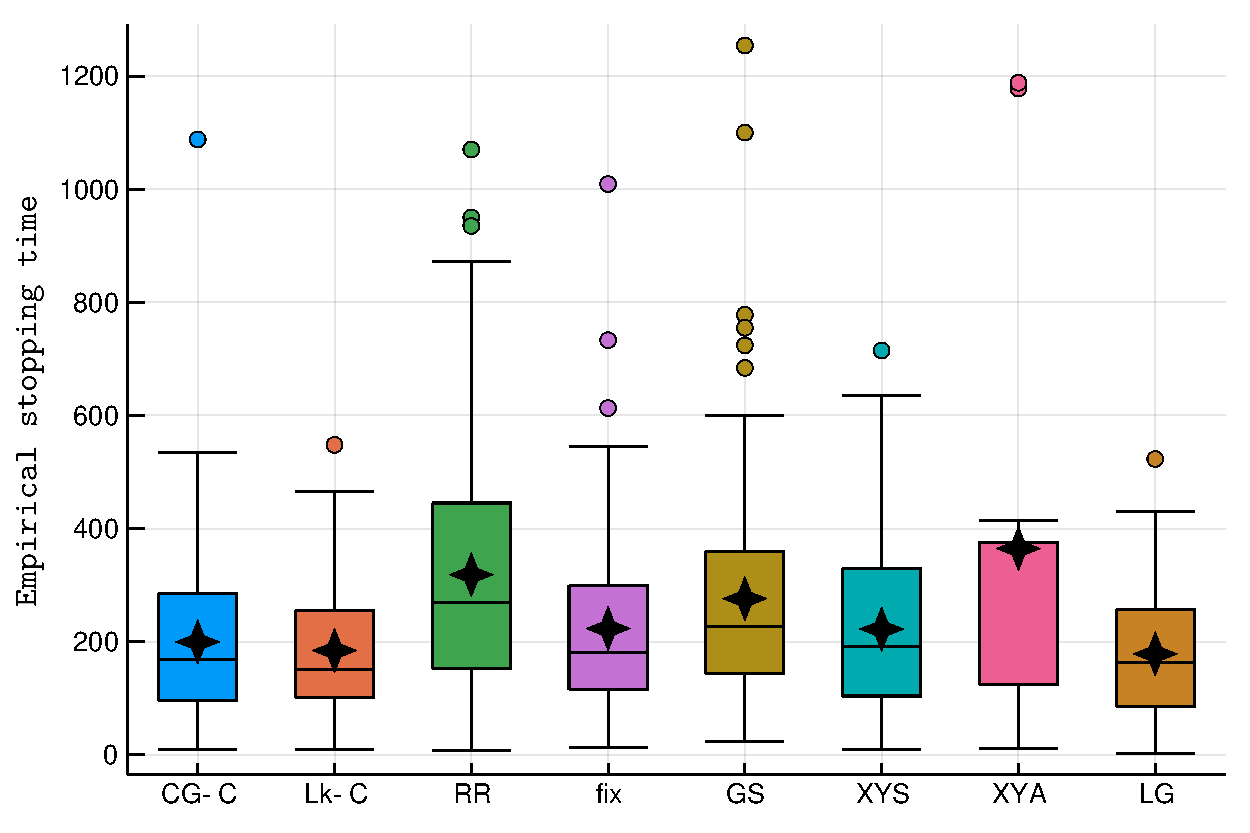
\includegraphics[clip, width= 0.33\textwidth]{Chapter4/img/bai_sin_0-1}
 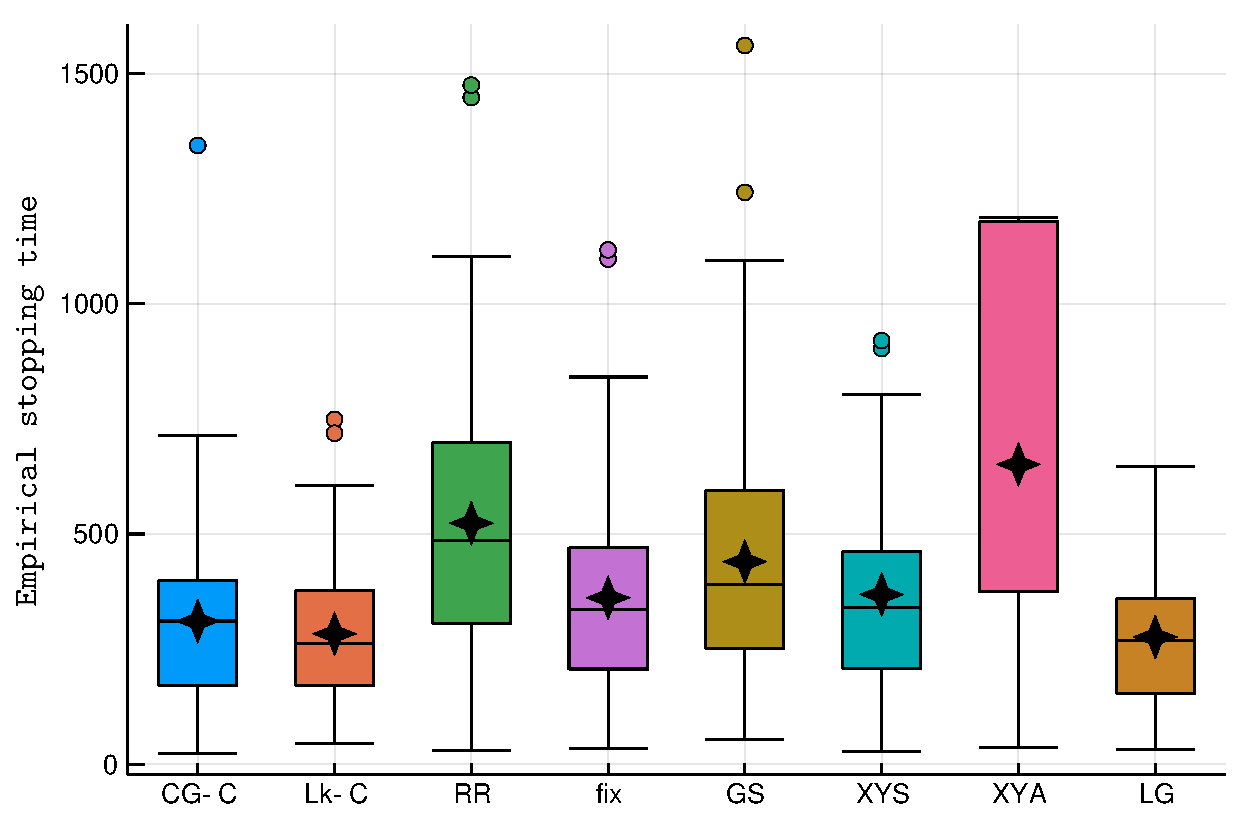
\includegraphics[clip, width= 0.33\textwidth]{Chapter4/img/bai_sin_0-01}
 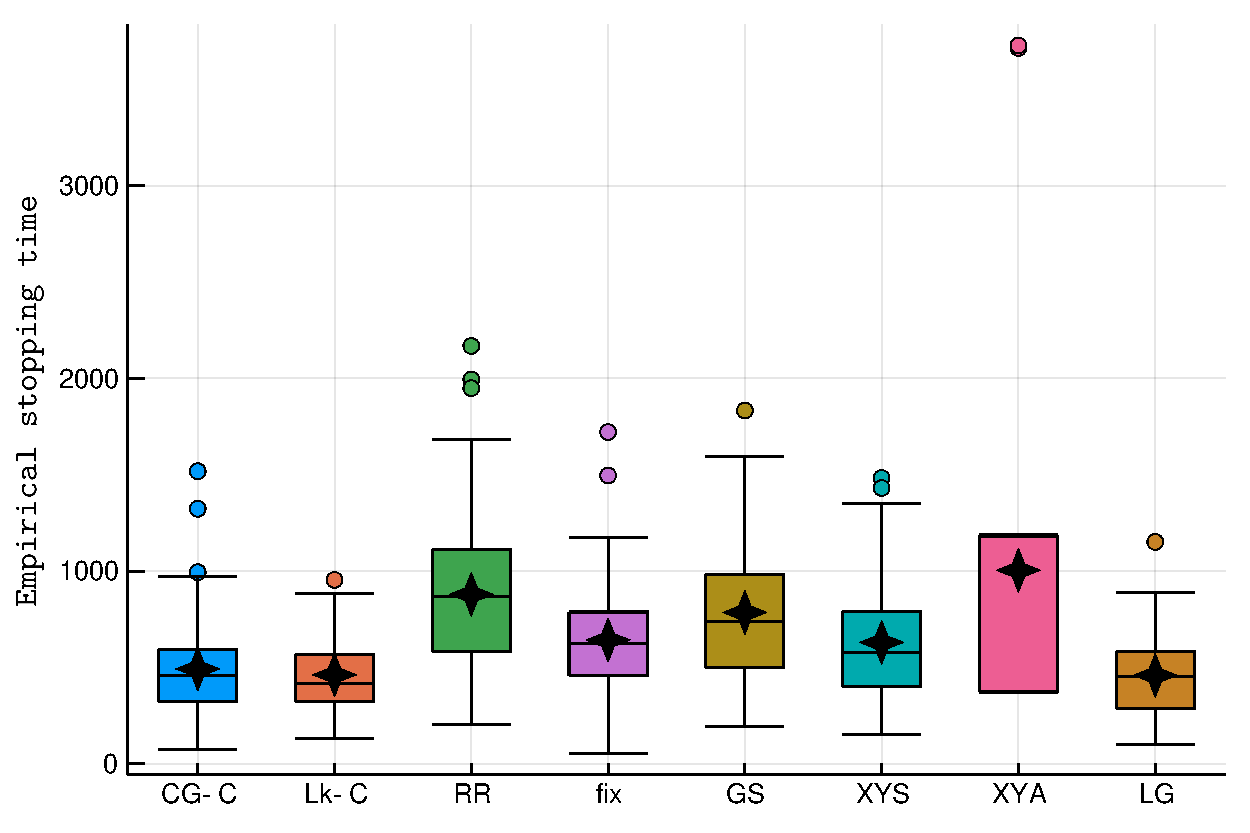
\includegraphics[clip, width= 0.33\textwidth]{Chapter4/img/bai_sin_0-0001}
 \caption{Sample complexity of different linear BAI sampling rules over the usual counter-example with $\delta=0.1, 0.01, 0.0001$ respectively. CG = \LGC,  Lk = \LG, RR = uniform sampling, fix = tracking the fixed weights, GS = \XYS with $\gopt$-allocation, XYS = \XYS with $\xyopt$-allocation, LG = \LGapE. The mean stopping time is represented by a black cross.}
 \label{fig:sample_complexity_1}
\end{figure}

For the second instance, we consider 20 arms randomly generated from the unit sphere $\mathbb{S}^{d-1}\eqdef\{a\in\R^d; \normm{a}_2=1\}$. We choose the two closest arms $a, a'$ and we set $\theta = a + 0.01(a'-a)$ so that a is the best arm. This setting has already been considered by~\citet{tao2018alba}. We report the same box plots over 100 replications as before with increasing dimension in Fig.~\ref{fig:sample_complexity_2}. More precisely, we set $d=6, 8, 10, 12$ respectively, and always keep a same $\delta = 0.01$. Our algorithms consistently show strong performances compared to other algorithms apart from \LGapE.
%Moreover, we can see that in these random examples, \LGC works better than the non-confexified one, and is even competitive compared to \LGapE.


\begin{figure}[ht]
 \centering
 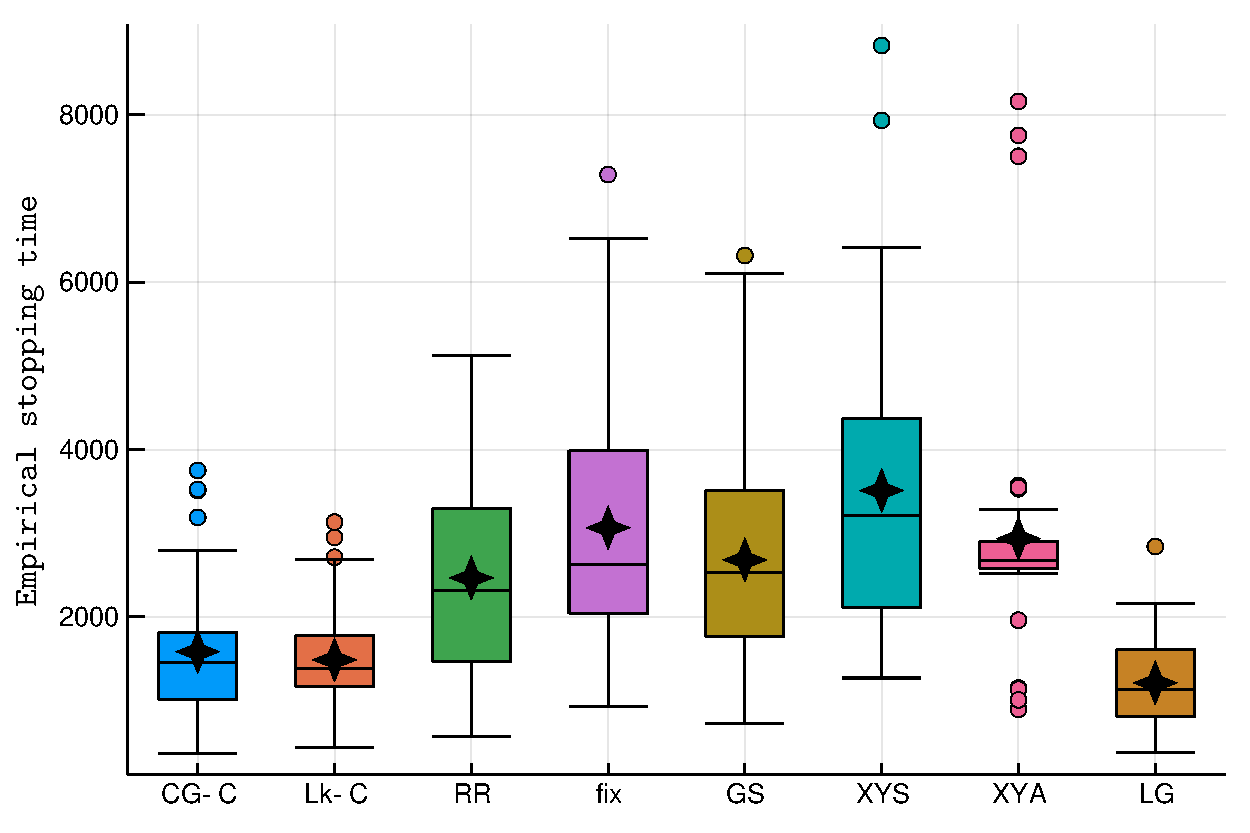
\includegraphics[clip, width= 0.33\textwidth]{Chapter4/img/bai_dim_6}
 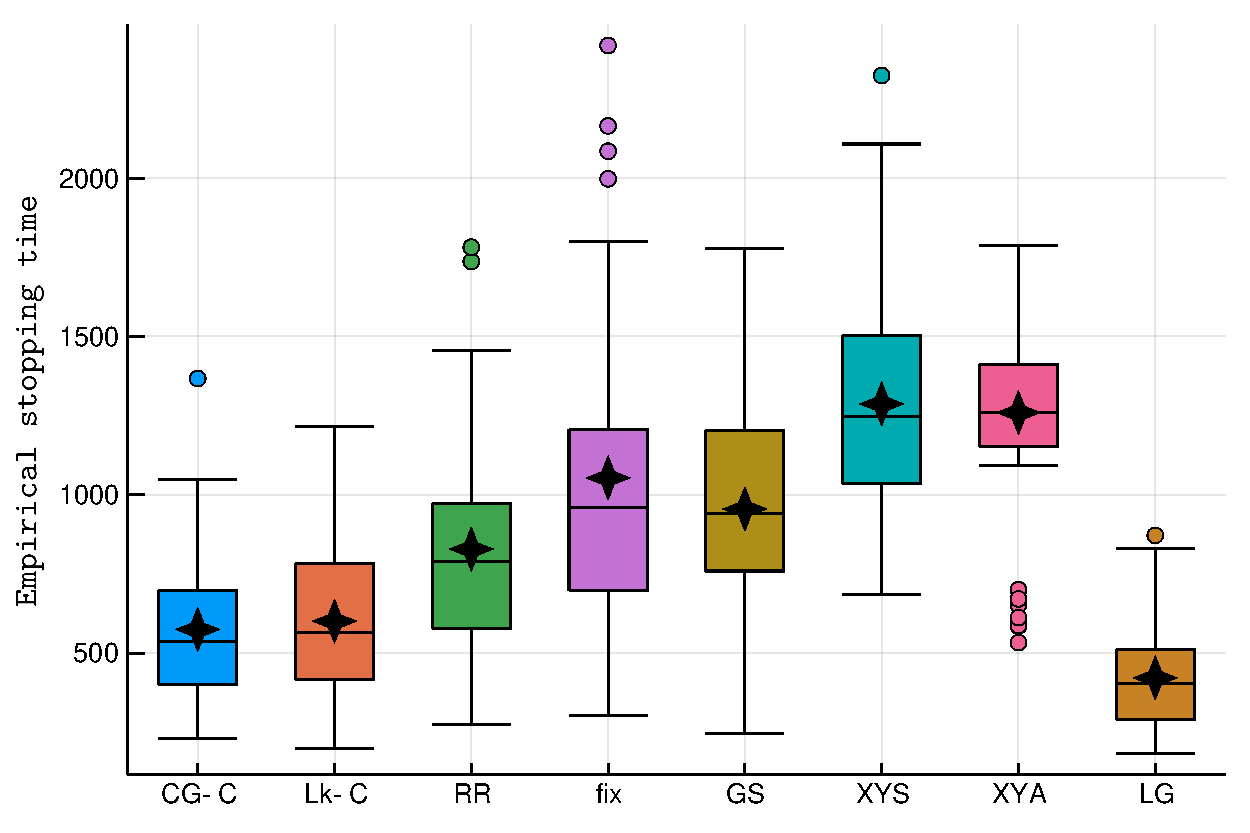
\includegraphics[clip, width= 0.33\textwidth]{Chapter4/img/bai_dim_8}
 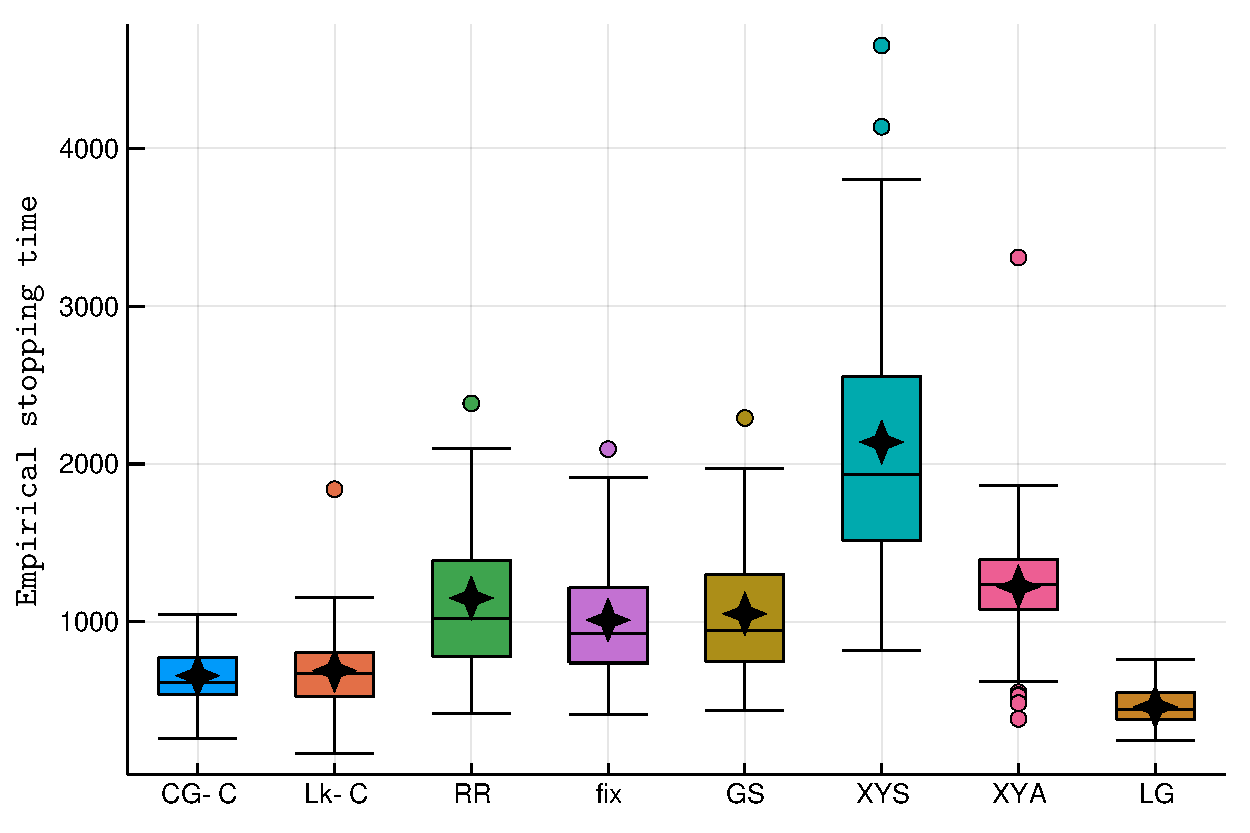
\includegraphics[clip, width= 0.33\textwidth]{Chapter4/img/bai_dim_10}
 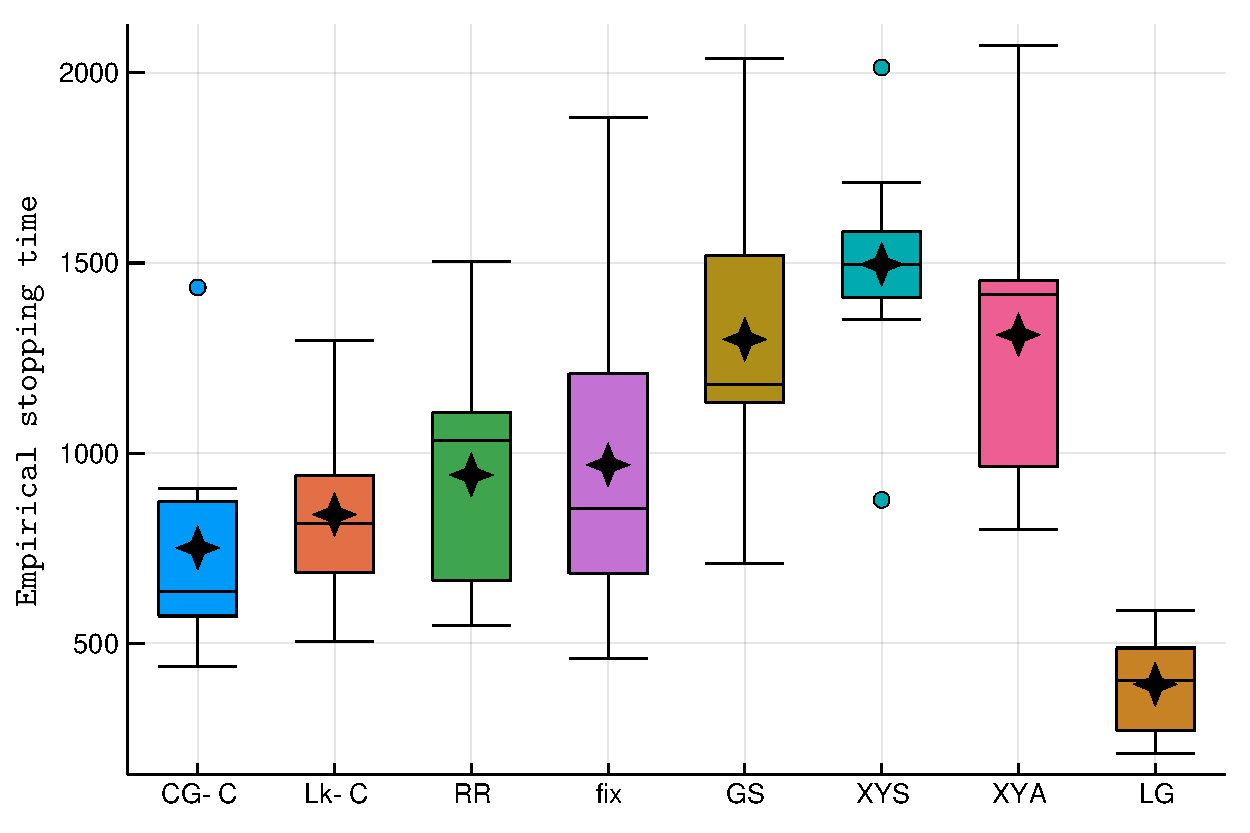
\includegraphics[clip, width= 0.34\textwidth]{Chapter4/img/bai_dim_12}
 \caption{Sample complexity of different linear BAI sampling rules over random unit sphere vectors with $d=6, 8, 10, 12$ from left to right.}
 \label{fig:sample_complexity_2}
\end{figure}

%We stress that although the main focus of this chapter is theoretical, with algorithms that are asymptotically optimal, our methods are also competitive with earlier algorithms experimentally.



\section{Adding Safety Constraints}\label{sec:lgc.safe}


%!TEX root = ../Chapter3.tex
\subsection{Bounded parameters}

We provide a bounded version of different examples (e.g. BAI) in Appendix~\ref{app:lgc.examples} where we add the assumption that the parameter set $\cM$ is bounded. In particular we show how it affects the lower bound of Theorem~\ref{th:lb_genral}: the characteristic time $\Tstar(\theta)$ is reduced (or equivalently $\Tstar(\theta)^{-1}$ increases). This is not surprising since we add a new constraint in the optimization problem. This means that the algorithm should stop earlier. The counterpart of this improvement is that it is often difficult to compute the best response for nature. Indeed, for example, in BAI, there is an explicit expression of the best response, see Appendix~\ref{app:lgc.examples.bai}. When the constraint $\normm{\lambda}\leq M$ is added there is no explicit expression anymore and one needs to solve an uni-dimensional optimization problem, see Lemma~\ref{lem:lagrange_alternative}. To devise an asymptotically optimal algorithm without the boundedness assumption remains an open problem.


% , i.e for $i\in\cI$ and $w\in\interior{\Sigma_A}$ in the interior of the probability simplex of dimension $A-1$, find $\lambda^i$ such that
% \[
% \lambda^i \in \argmin_{\lambda\neg i}\normm{\theta - \lambda }_{V_{w}}\,.
% \]
% For example, in BAI, there is an explicit expression of the best response. Noting that, for $\astar\in\cA$, we have
% \[
% \min_{\lambda\neg \astar}\normm{\theta - \lambda }_{V_{w}} = \min_{a\neq \astar}\min_{\langle\lambda,a-\astar\rangle>0} \normm{\theta - \lambda }_{V_{w}}\,,
% \]
% the best response is then
% \begin{align}
% \lambda^{b} &= \theta - \frac{\max(\langle\theta,\astar-b \rangle,0) }{\normm{\astar-b}_{V_w^{-1}}^2} V_w^{-1}(\astar - b) \label{eq:best_response_bai}
% \\
% \text{for }b&\in\argmin_{a\neq \astar}\normm{\theta - \lambda^{a} }_{V_{w}}\nonumber.
% \end{align}
% When the constraint $\normm{\lambda}\leq M$ is added there is no explicit expression anymore and one needs to solve an uni-dimensional optimization problem, see Lemma~\ref{lem:lagrange_alternative}.


Note that in the proof of Theorem~\ref{thm:sample_complexity} we only use two times the boundedness assumption, first in the definition of the threshold $\beta(t,\delta)$ (see Theorem~\ref{th:confidence_beta}) to handle the bias induced by the regularization. Second, since the regret of AdaHedge is proportional to the maximum of the upper confidence bounds $U_s^{i,a}$, we need to ensure that they are bounded.

% And there exists pathological pure exploration problems where even the quantity uppper bounded by $U_s^{i,a}$, namely $\normm{\theta-\lambda}_{aa^\top}^2$ where $\lambda\in\argmin_{\lambda'\in\neg i}\normm{\theta -\lambda}$ is unbounded\todo{I don't understand what this means.}. See for example Appendix~G.3 by \citet{menard2019lma}.


%!TEX root = ../Chapter4.tex
\section{Related Work}\label{sec:lgc.related_work}

We survey previous work on linear BAI. The major focus is put on sampling rules in this section. We stress that all the stopping rules employed in the linear BAI literature are equivalent up to the choice of their exploration rate (More discussion in Appendix~\ref{app:lgc.stopping}). As aforementioned, existing sampling rules are either based on \SE or \UGapE. Elimination-based sampling rules usually operate in phases and progressively discard sub-optimal directions. Gap-based sampling rules always play the most informative arm that reduces the uncertainty of the gaps between the empirical best arm and the others.

\paragraph{\XYS and \XYA.} \citet{soare2014linear} first propose a static allocation design \XYS that aims at reducing the uncertainty of the gaps of all arms. More precisely, it requires to either solve the $\xyopt$-complexity or use a \emph{greedy} version that pulls the arm 
\[
    \argmin_{\bx\in\cX} \max_{\by\in\cY_{\texttt{dir}}} \normm{\by}_{\bLambda_{\bomega}^{-1}}^2
\]
at the cost of having no guarantees. An elimination-like alternative called \XYA is proposed then to overcome that issue. We say elimination-like since \XYA does not discard arms once and for all, but reset the active arm set at each phase. These two algorithms are the first one being linked to $\gopt$-optimality, but are not asymptotically optimal.

\paragraph{\ALBA.} \ALBA is also an eliminations-based algorithm designed by~\citet{tao2018alba} that improves over \XYA by a factor of $d$ in the sample complexity using a tighter elimination criterion.
\vspace{-0.2cm}

\paragraph{\RAGE.} \citet{fiez2019transductive} extend \XYS and \XYA to a more general transductive bandits setting. \RAGE is also elimination-based and requires the computation of $\xyopt$-complexity at each phase.

\paragraph{\LGapE and variants.} \LGapE~\citep{xu2018linear} is the first gap-based sampling rule for linear BAI. \LGapE is inspired by \UGapE~\citep{gabillon2012ugape}. It is, however, not clear whether \LGapE is asymptotically optimal or not. Similar to \XYS, \LGapE either requires to solve a time-consuming optimization problem at each step, or can use a greedy version that pulls arm 
\[
    \argmin_{\bx\in\cX} \normm{\bx_{i_n}-\bx_{j_n}}_{(\bA_n+\bx\bx\transpose)^{-1}}^2
\]
instead, again at the cost of losing guarantees. Here $i_n = \Istar(\hat\btheta_n)$ and $\hbx_{j_n}$ is the most ambiguous arm w.r.t. $\hbx_{i_n}$, i.e. 
\[
    \argmax_{j\neq i_n} (\bx_{j}-\bx^\star(\hat\btheta_n^\lambda))\transpose\hat\btheta_n^\lambda + \normm{\bx^\star(\hat\btheta_n^\lambda) - \bx_{j_n}}_{\bA_n^{-1}} \sqrt{2d_{n,\delta}}\,,
\]
with $d_{n,\delta}$ the stopping rule threshold.

On the other hand,~\citet{zaki2019maxoverlap} propose a new algorithm based on \LUCB. With a careful examination, we note that the sampling rule of \GLUCB is equivalent to that of the greedy \LGapE using the Sherman-Morrison formula. Later, \citet{kazerouni2019glb} provide a natural extension of \LGapE to the \emph{generalized linear bandits} setting, where the rewards depend on a strictly increasing \emph{inverse link function}. \GLGapE reduces to \LGapE when the inverse link function is the identity function.

\paragraph{Summary.}
It is worth noting that all the sampling rules presented here depend on $\delta$ (except \XYS), while we aim to design sampling rules that are $\delta$-free which is appealing for applications as argued by~\citet{jun2016atlucb}. Also all the guarantees in the literature are of the form $C\log(\delta) + O\big(\log(1/\delta)\big)$ for a constant $C$ that is strictly larger than $\Tstar(\theta)^{-1}$.

In the next, we present a set of algorithms using different design patterns that aim to address linear bandits BAI, whilst trying to be asymptotically optimal.


%\input{Chapter4/sections/sec_analysis}  % this part got absorbed into the "algorihtm" section.

%!TEX root = ../Chapter4.tex

\section{Experiments}\label{sec:lgc.experiments}

In this section, we provide technical details of our experiments. We also share a few insights over different aspects of implementations of different pure exploration linear bandits algorithms. In particular, we propose a new Frank-Wolfe-typed heuristic to solve generic $\cA\cB$-design.

Besides our algorithms, we implement the following algorithms, all using the same stopping rule (more discussion given in Appendix~\ref{app:lgc.stopping}): uniform sampling, the greedy version of \XYS (including $\gopt$-allocation and $\xyopt$-allocation), \XYA, and the greedy version of \LGapE. We skip \GLUCB/\GLGapE since they are more or less equivalent to \LGapE in the scope of this paper.

\subsection{Implementation details}\label{sec:lgc.experiments.implem}

\paragraph{More details for algorithm implementations.} We give more clarifications on each individual algorithm implemented.

\begin{itemize}
	\item For our algorithms \LG and \LGC, we implemented the version with the boundedness assumption.
	\item For \LGapE We implemented the greedy version, that is, pull the arm 
	\[
	    \argmin_{a\in\cA} \normm{a_{i_t}-a_{j_t}}_{(V_{N_t}+aa^\top)^{-1}}^2
	\]
	with $i_t = i^\star(\hat\theta_t)$ and $j_t = \argmax_{j\neq i_t}\langle\hat\theta_t,a_{j}-a^\star(\hat\theta_t)\rangle + \normm{a^\star(\hat\theta_t) - a_{j_t}}_{V_{N_t}^{-1}} \sqrt{2\beta(t,\delta)}$. Note that this version does not have a theoretical guarantee in the general case. However, as we stated in Section~\ref{sec:lgc.related_work}, the \GLUCB proposed by~\citet{zaki2019maxoverlap} is equivalent to this greedy version of \LGapE, and they provided an analysis for the 2-arm and 3-arm case. \LGapE is designed for $\epsilon$-best-arm identification, we set $\epsilon=0$ in our experiments to make sure that it outputs the optimal one.
	\item For \XYS, we implemented the greedy incremental version for both $\gopt$-allocation and $\xyopt$-allocation, that allows us to avoid the optimal design-computing step. To implement the non-greedy version, readers are invited to look at next Section~\ref{sec:lgc.experiments.complexity} where we discuss in detail the computation of $\cA\cB$-optimal design.
	\item For \XYA, it requires a hyper-parameter that characterizes the length of each phase. We set that hyper-parameter to $0.1$ as done by~\citet{soare2014linear}.
\end{itemize}

\paragraph{Technical details.} All the algorithms and experiments are implemented in \lstinline{Julia 1.3.1}, and plots are generated using the \lstinline{StatsPlots.jl} package. Other external dependencies are: \lstinline{JLD2.jl, Distributed.jl, IterTools.jl, CPUTime.jl, LaTeXStrings.jl}.

\paragraph{For reproducibility.} To rerun our code, your need to have Julia installed, then unzip \lstinline{code.zip} and do the following in your terminal.

\begin{lstlisting}
  $ cd PATH/TO/THE/FOLDER/code/linear
  $ julia
  julia> include("experiment_bai1.jl") # reproduce Fig.1
  julia> include("viz_bai1.jl") # visualization
  julia> include("experiment_bai2.jl") # reproduce Fig.2
  julia> include("viz_bai2.jl") # visualization
\end{lstlisting}

%\subsubsection{Arm generation.} In Section~\ref{sec:experiments}, we need to generate arms uniformlly from a unit sphere of arbitrary dimension. This can be done using Algorithm~\ref{alg:generation}, it can be trivially extended to higher dimension.
%
%\begin{algorithm}[ht]
%   \caption{Generating arms from the 2D unit sphere (Box-Mueller)}
%   \label{alg:generation}
%\begin{algorithmic}
%        \State $u \sim \cN(0,1)$
%        \State $v \sim \cN(0,1)$
%        \State $(x, y) = (u, v)/\normm{(x, y)}_2$
%        \RETURN $x, y$
%\end{algorithmic}
%\end{algorithm}

\subsection{Computation of different complexities}\label{sec:lgc.experiments.complexity}

As mentioned in Section~\ref{sec:lgc.lower_bound}, computing the solution to a specified optimization problem is required in many existing linear BAI algorithms. We survey some methods that can potentially be useful to handle that issue.

We recall that the three notions of complexity $\gopt, \xyopt, \cA\cBstar(\theta)$ can be written in a unified form,
\begin{align}\label{eq:complexity_general}
    \cA\cB = \min_{w\in\Sigma_A} \max_{b\in\cB}\normm{b}_{V_w^{-1}}^2,
\end{align}
where $\cB$ is the transductive set, i.e. a finite set of elements in $\R^d$. Transductive sets corresponding to different complexity types mentioned in this paper can be found in Table~\ref{tab:transductive_sets}.

\begin{table}[ht]
    \centering
	\begin{tabular}{@{}lll@{}}
		\toprule
		\thead{Allocation type} & \thead{Arm set} & \thead{Transductive set} \\ \midrule
		(1) $\gopt$-allocation & $\cA$ & $\cA$\\
		(2) $\xyopt$-allocation & $\cA$ & $\cB_{\texttt{dir}} = \{a-a':\ (a,a')\in\cA\times\cA\}$ \\
		(3) $\cA\cBstar(\theta)$-allocation & $\cA$ & $\cB^\star(\theta) = \left\{ (\astar(\theta)- a)/\left|\big\langle \theta, \astar(\theta)-a\big\rangle\right|: a\in\cA/\big\{\astar(\theta)\big\}  \right\}$ \\
		\bottomrule
	\end{tabular}
	\caption{Some examples of different transductive sets.}
	\label{tab:transductive_sets}
\end{table}

\paragraph{Frank-Wolfe.} We can use a Frank-Wolfe heuristic to compute the optimizer of~\eqref{eq:complexity_general} shown in Algorithm~\ref{alg:fw_aa}. This heuristic is used for example by~\citet{fiez2019transductive}. Note that this heuristic has been proved to have a linear convergence guarantee when $\cB = \cA$~\citep{ahipasaoglu2008fw}. It is not clear, however, that the same guarantee holds for other transductive sets.

A simple sanity check to test whether a solver works smoothly is  to solve $\cA\cBstar(\theta)$ for classical multi-armed bandits (i.e. when $\cA= \{e_1,e_2,\ldots,e_d\}$), for which a solver with guarantee exists (see \citealt{garivier2018explore}). In particular we found instances where Algorithm~\ref{alg:fw_aa} does not converge toward the optimal weights, for example: $\cA= \{e_1,e_2,e_3\}, \theta = (0.9, 0.5, 0.5)$.

% \begin{algorithm}[ht]
%    \caption{Frank-Wolfe heuristic for computing $\gopt$-design}
%    \label{alg:fw_aa}
% \begin{algorithmic}
%    \State {\bfseries Input:} arm set $\cA\subset\R^d$, transductive set $\cB\subset\R^d$, maximum iterations $n$
%    \State  {\bfseries Initialize:} $w \leftarrow{} (1/A, 1/A, \ldots, 1/A), V \leftarrow{} I_d, t \leftarrow{} 0$
%    \While{$t<n$}
%         \State $i_{t}\in\argmin_{i\in\{1,\ldots,A\}}\max_{b\in\cB}\normm{b}^2_{(V+a_i a_i^\top)^{-1}}$
%         \State $V \leftarrow{} V + a_{i_{t}}a_{i_{t}}^\top$
%         \State $w \leftarrow{} \frac{t}{t+1}w+\frac{1}{t+1}e_{i_{t}}$
%         \State $t \leftarrow{} t+1$
%    \EndWhile
%    \RETURN $w$
% \end{algorithmic}
% \end{algorithm}


\begin{algorithm}[ht]
\centering
\caption{Frank-Wolfe heuristic for computing $\gopt$-design}
\label{alg:fw_aa}
\begin{algorithmic}
   \State {\bfseries Input:} arm set $\cA\subset\R^d$, transductive set $\cB\subset\R^d$, maximum iterations $n$
   \State  {\bfseries Initialize:} $w \leftarrow{} (1, 1, \ldots, 1)\in\R^A, V \leftarrow{} I_d, t \leftarrow{} 0$
   \While{$t<n$}
        \State $\ta\in\argmin_{a\in\cA}\max_{b\in\cB}\langle a,b\rangle_{V^{-1}}^2$%\normm{b}^2_{(V+a_i a_i^\top)^{-1}}$
        \State $V \leftarrow{} V + \ta \ta^\top$
        \State $w \leftarrow{} \frac{t}{t+1}w+\frac{1}{t+1}e_{\ta}$
        \State $t \leftarrow{} t+1$
   \EndWhile
   \State {\bfseries Return} $w$
\end{algorithmic}
\end{algorithm}

We propose a variant of the previous heuristic that takes into account a count for each element in the transductive set $\cB$. The pseudo-code of our method is displayed in Algorithm~\ref{alg:fw_ab}. $N\in\NN^{|\cB|}$ denotes the vector of counts for all $b\in\cB$. Sanity check on various MAB instances shows the correctness of our heuristic, its convergence guarantee remains for the future work.

% \begin{algorithm}[ht]
%    \caption{Saddle Frank-Wolfe heuristic for computing generic $\cA\cB$-design}
%    \label{alg:fw_ab}
% \begin{algorithmic}
%    \State {\bfseries Input:} arm set $\cA\subset\R^d$, transductive set $\cB\subset\R^d$, maximum iterations $n$
%    \State  {\bfseries Initialize:} $w \leftarrow{} (1/A, 1/A, \ldots, 1/A), N \leftarrow{} (1, 1, \ldots, 1), V \leftarrow{} I_d, t \leftarrow{} 0$
%    \While{$t<n$}
%         \State $i_{t}\in\argmin_{i\in\{1,\ldots,A\}}\sum_{j=1}^B(-2N[j]\langle a_i,V b_j\rangle^2)$
%         \State $j_{t}\in\argmax_{j\in\{1,\ldots,B\}}\normm{b_{j}}^2_{V^{-1}}$
%         \State $V \leftarrow{} V + a_{i_{t}}a_{i_{t}}^\top$
%         \State $N[j_t] \leftarrow{} N[j_t] + 1$
%         \State $w \leftarrow{} \frac{t}{t+1}w+\frac{1}{t+1}e_{i_{t}}$
%         \State $t \leftarrow{} t+1$
%    \EndWhile
%    \RETURN $w$
% \end{algorithmic}
% \end{algorithm}

\begin{algorithm}[ht]
\centering
\caption{Saddle Frank-Wolfe heuristic for computing generic $\cA\cB$-design}
\label{alg:fw_ab}
\begin{algorithmic}
   \State {\bfseries Input:} arm set $\cA\subset\R^d$, transductive set $\cB\subset\R^d$, maximum iterations $n$
   \State  {\bfseries Initialize:} $w \leftarrow{} (1, 1, \ldots, 1)\in\R^A, \tV \leftarrow{} I_d, V \leftarrow{} I_d, t \leftarrow{} 0$
   \While{$t<n$}
        \State $\ta\in\argmax_{a\in\cA}  \norm{a}_{V^{-1} \tV V^{-1} }^2$
        \State $\tb\in\argmax_{b\in\cB}\normm{b}^2_{V^{-1}}$
        \State $V \leftarrow{} V + \ta\ta^\top$
		\State $\tV \leftarrow{} \tV + \tb\tb^\top$
        \State $w \leftarrow{} \frac{t}{t+1}w+\frac{1}{t+1}e_{\ta}$
        \State $t \leftarrow{} t+1$
   \EndWhile
   \State {\bfseries Return} $w$
\end{algorithmic}
\end{algorithm}

\paragraph{Entropic mirror descent.}
An entropic mirror descent alternative is used by~\citet{tao2018alba} to compute $\gopt$. The entropic mirror descent approach requires the knowldge of the Lipschitz constant of $\log\det V_w$. Unfortunately, that Lipschitzness property does not seem to hold. \citet{lu2018convex} propose a solution to overcome the Lipschitz issue, but only for $\gopt$-design. Whether it still works for general $\cA\cB$-design remains an open question.

%\begin{algorithm}[ht]
%   \caption{Entropic mirror descent heuristic for computing $\gopt$-design}
%   \label{alg:algoMD}
%\begin{algorithmic}
%   \State {\bfseries Input:} arm set $\cA\subset\R^d$, transductive set $\cB\subset\R^d$, tolerance constant $\epsilon$, Lipschitz constant $L$
%   \State  {\bfseries Initialize:} $w \leftarrow{} (1/A, 1/A, \ldots, 1/A), t \leftarrow{} 1$
%   \While{$|\max_{a\in\cA}a^\top V_w^{-1} a - d| \geq \epsilon$}
%        \State $\gamma \leftarrow{} \frac{2\sqrt{A}}{L} \frac{1}{\sqrt{t}}$
%        \State Compute gradient $\nabla^i \leftarrow{} \Tr(V_w^{-1}a_ia_i^\top)$
%        \State $w^{a_i} \leftarrow{} \frac{w^{a_i}\exp(\gamma \nabla^i)}{\sum_{i=1}^A w^{a_i}\exp(\gamma \nabla^i)}$
%        \State $t \leftarrow{} t+1$
%   \EndWhile
%   \RETURN $w$
%\end{algorithmic}
%\end{algorithm}

\subsection{Implementation tricks}\label{sec:lgc.experiments.tricks}

\paragraph{Rank-1 matrix inversion and posterior update.}
Matrix inversion is a costly step that should be avoided at best. For linear bandits, in particular, we need to inverse the (regularized) design matrix $\bB^{\lambda}_n$, which is renewed with a rank-1 update at each time step. Applying Sherman-Morrison formula allows us thus to only update its inverse incrementally, that releases a huge burden of computation.

Indeed, beginning with $\bB^{\lambda}_0 \eqdef \lambda\1_d$, we have
\[
    \forall t\geq 0, \quad \bB^{\lambda}_{t+1} = \bB^{\lambda}_t + \hat{\bx}_{t+1}\hat{\bx}_{t+1}\transpose,
\]
thus using Sherman-Morrison formula we have
\[
    \forall t\geq 0, \quad (\bB^{\lambda}_{t+1})^{-1} = (\bB^{\lambda}_t)^{-1} - \frac{(\bB^{\lambda}_t)^{-1}\hat{\bx}_{t+1}\hat{\bx}_{t+1}\transpose(\bB^{\lambda}_t)^{-1}}{1+\normm{\hat{\bx}_{t+1}}_{(\bB^{\lambda}_t)^{-1}}^2}.
\]

The posterior mean vector and covariance matrix can then be easily expressed in terms of $(\bB^{\lambda}_t)^{-1}$. Let $\bz_t \eqdef \sum_{s=1}^t y_s\hat{\bx}_s$, we obtain
\[
    \hat{\btheta}_n^{\lambda} = (\bB^{\lambda}_t)^{-1}\bz_t \quad \text{and} \quad \hat{\bSigma}_n = \sigma^2 (\bB^{\lambda}_t)^{-1}.
\]

\paragraph{Rank-1 multivariate normal distribution sampling}
A random Gaussian vector 
\[
    \bX = (X_1, X_2, \ldots, X_d)\transpose
\] 
of mean vector $\bar{\bmu}$ and covariance matrix $\bSigma$ can be formally defined as following,
\[
    \bX \sim \cN(\bar{\bmu}, \bSigma) \iff \exists \bar{\bmu}\in\mathbb{R}^d,\bA\in\mathbb{R}^{d\times d'} \ \text{s.t.} \ \bX = \bA \mathbf{Z} + \bar{\bmu},
\]
for $Z_i \sim\ \mathcal{N}(0, 1)$ i.i.d. with $i\in\{1,\ldots,d'\}$, and here $\bSigma = \bA\bA\transpose$.

To draw a sample from a multivariate normal distribution, according to the previous definition, one can first find any real matrix $\bA$ such that $\bA\bA\transpose = \bSigma$. Then draw a vector $\bZ$ whose components independently follow standard normal distribution. Finally $\bX = \bA \mathbf{Z} + \bar{\bmu}$ forms a valid sample. The main issue is thus how to find an appropriate matrix $\bA$.

In this chapter, we need to sample from $\cN(\hat{\btheta}^\lambda_n,\hat{\bSigma}_n)$ for \LTCC{} for example, where the covariance matrix $\hat{\bSigma}_n$ is a positive-definite matrix. A usual way is to apply the Cholesky decomposition, which is computationally inefficient if it were to be applied at each time step. Fortunately, we can apply rank-1 Cholesky decomposition in our case.  

%We, however, notice that $\bA = (\hat{\bSigma}_n)^{1/2}=\sigma(\bB^{\lambda}_n)^{-1/2}$ is also a valid candidate, and is thus can be also updated iteratively using a similar formula to the Sherman-Morrison formula.

%More precisely, we have
%\begin{align*}
%    \forall t\geq 0, \quad (\bB^{\lambda}_{t+1})^{-\frac{1}{2}} = (\bB^{\lambda}_t)^{-\frac{1}{2}} - \ddfrac{\left(1-\sqrt{1-\frac{\normm{\hat{\bx}_{t+1}}_{(\bB^{\lambda}_t)^{-1}}^2}{1+\normm{\hat{\bx}_{t+1}}_{(\bB^{\lambda}_t)^{-1}}^2}}\right)}{\normm{\hat{\bx}_{t+1}}_{(\bB^{\lambda}_t)^{-1}}^2} (\bB^{\lambda}_t)^{-\frac{1}{2}}\hat{\bx}_{t+1}\hat{\bx}_{t+1}\transpose(\bB^{\lambda}_t)^{-\frac{1}{2}}.
%\end{align*}

\subsection{Experimental setting}\label{sec:lgc.experiments.setting}

\paragraph{The usual hard instance.}
Usual sampling rules for classical BAI may not work for the linear case. This can be understood on a well-studied instance already discussed by~\citet{soare2014linear,xu2018linear}, which encapsulates the difficulty of BAI in a linear bandit, and thus is the first instance on which we test our algorithms. In this instance, arms are the canonical basis  $a_1 = e_1, a_2 = e_2, a_d = e_d$, plus an additional disturbing arm $a_{d+1} = (\cos(\alpha), \sin(\alpha), 0, \ldots, 0)^\top$, and a true regression parameter $\theta$ equal to $e_1$. In this problem, the best arm is always $a_1$, but when the angle $\alpha$ is small, the disturbing arm $a_{d+1}$ is hard to discriminate from $a_1$. As already argued by~\citet{soare2014linear}, an efficient sampling rule for this problem instance would rather pull $a_2$ in order to reduce the uncertainty in the direction $a_1-a_{d+1}$. Naive adaptation of classical BAI algorithms cannot deal with that situation naturally. We further use a simple set of experiments to justify that intuition. We run our two algorithms and the one of~\citet{degenne2019game} that we call \texttt{DKM} over the problem instance whence $d=2$, $\delta=0.01$ and $\alpha=0.1$. We show the number of pulls for each arm averaged over 100 replications of experiments in Table~\ref{table:pulls}. We see that, indeed, \texttt{DKM} pulls too much $a_3$, while our algorithms focus mostly on $a_2$.

\begin{table}[t!]\centering
%\def\arraystretch{1.2}
\begin{tabular}{|c|c|c|c|}
 \hline
 & \LG & \LGC & \texttt{DKM} \\
 \hline
 \textbf{$a_1$} & $1912$ & $1959$ & $1943$ \\
 \hline
 \textbf{$a_2$} & $5119$ & $4818$ & $4987$ \\
 \hline
 \textbf{$a_3$} & $104$ & $77$ & $1775$ \\
 \hline
 \textbf{Total} & $7135$ & $\bf{6854}$ & $8705$ \\
 \hline
\end{tabular}
\caption{Average number of pulls of \LG and \LGC (against \texttt{DKM}) for each arm.}
\label{table:pulls}
\end{table}

\subsection{Experimental results}\label{sec:lgc.experiments.results}

\paragraph{Comparison of different complexities.}
We use the previous setting to illustrate various complexities differ in practice. In Table~\ref{table:optimal_weights} we compare the different complexities mentioned in this paper: the characteristic time $\Tstar(\theta)$ and its associated optimal weights $\wstar_{\cA\cBstar(\theta)}$, the $\xyopt$-complexity and its associated optimal design $\wstar_{\xyopt}$, the G-optimal complexity $\gopt$ and its associated optimal design $\wstar_{\cA\cA}$. For each weight vector $w \in\{\wstar_{\cA\cBstar(\theta)},w_{\xyopt}, w_{\gopt}\}$,
 we also provide the lower bound $T_w$ given by Theorem~\ref{th:lb_genral}, i.e.
 \[
 T_w = \max_{a\neq \astar(\theta)} \frac{\big\langle \theta, \astar(\theta)-a\big\rangle^2}{2\normm{\astar(\theta)-a}_{V_w^{-1}}^2} \log(1/\delta).
\]
In particular we notice that targeting the proportions of pulls $w_{\xyopt}, w_{\gopt}$ leads to a much larger lower bound than the one obtained with the optimal weights.
\begin{table}[t!]
\centering
%\def\arraystretch{1.2}
\begin{tabular}{|c|c|c|c|}
 \hline
   & $\wstar_{\cA\cBstar}$ & $\wstar_{\xyopt}$  & $\wstar_{\gopt}$   \\
 \hline
 \textbf{$a_1$} & $0.047599$ & $0.499983$ & $0.499983$ \\
 \hline
 \textbf{$a_2$} & $0.952354$ & $0.499983$ & $0.499983$ \\
 \hline
 \textbf{$a_3$} & $0.000047$ & $0.000033$ & $0.000033$ \\
 \hline
 \textbf{$T_w$} & $369$ & $2882$ & $2882$ \\
 \hline
   & $\Tstar(\theta)$ & $2\xyopt/\DeltaMin^2$ & $8\gopt/\DeltaMin^2$\\
 \hline
  \textbf{Complexity} & $0.124607$ & $32.0469$ & $64.0939$ \\
 \hline
\end{tabular}
\caption{Optimal weights for various complexities with $\DeltaMin= 0.0049958$.}
\label{table:optimal_weights}
\end{table}

\paragraph{Comparison with other algorithms.}
Finally we benchmark our two sampling rules against others from the literature. %Note that the main purpose of this paper is to propose algorithms with asymptotic optimality while being practically usable, but we do not claim to have the best performing ones.
We test over two synthetic problem instances, with the first being the previous counter-example. We set $d=2$, $\alpha=\pi/6$. Fig.~\ref{fig:sample_complexity_1} shows the empirical stopping time of each algorithms averaged over 100 runs, with a confidence level $\delta=0.1, 0.01, 0.0001$ from left to right. Our two algorithms show competitive performance (the two leftmost boxes on each plot), and are only slightly worse than \LGapE.

\begin{figure}[ht]
 \centering
 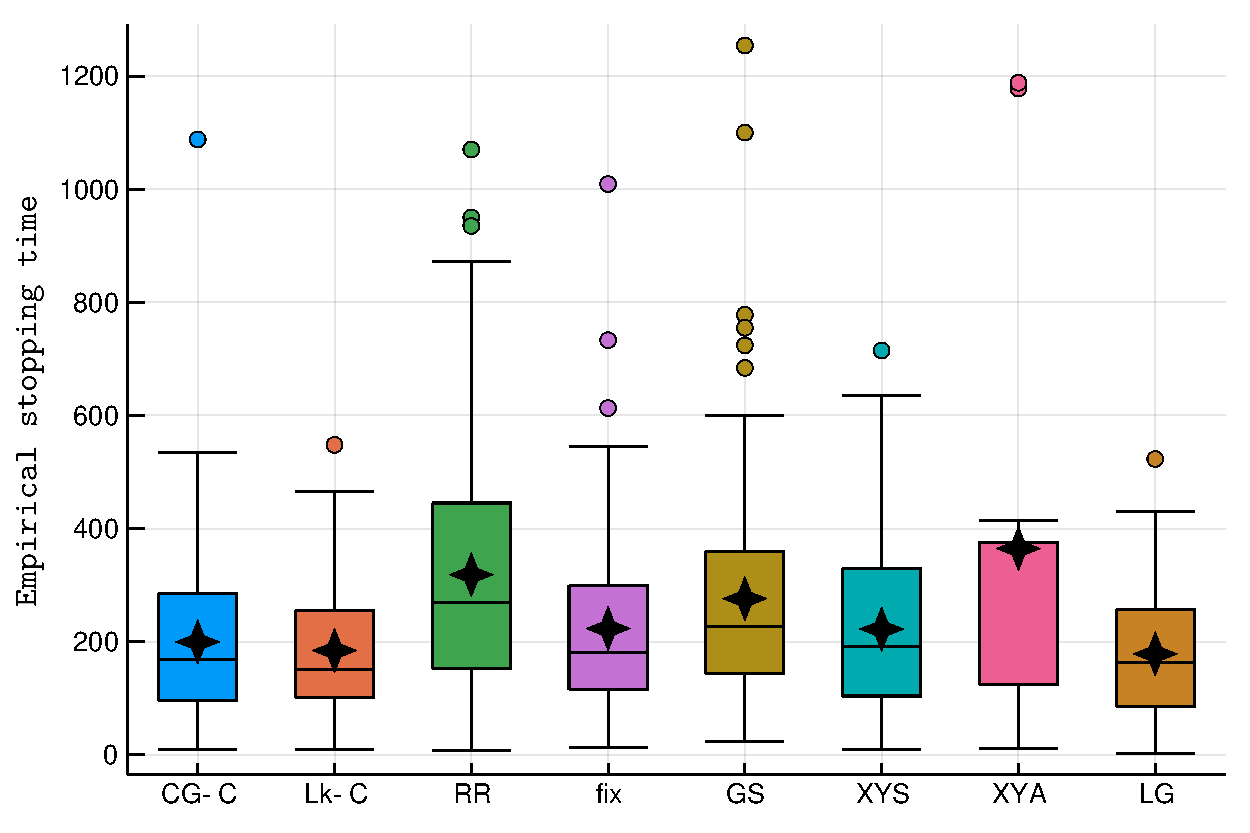
\includegraphics[clip, width= 0.33\textwidth]{Chapter4/img/bai_sin_0-1}
 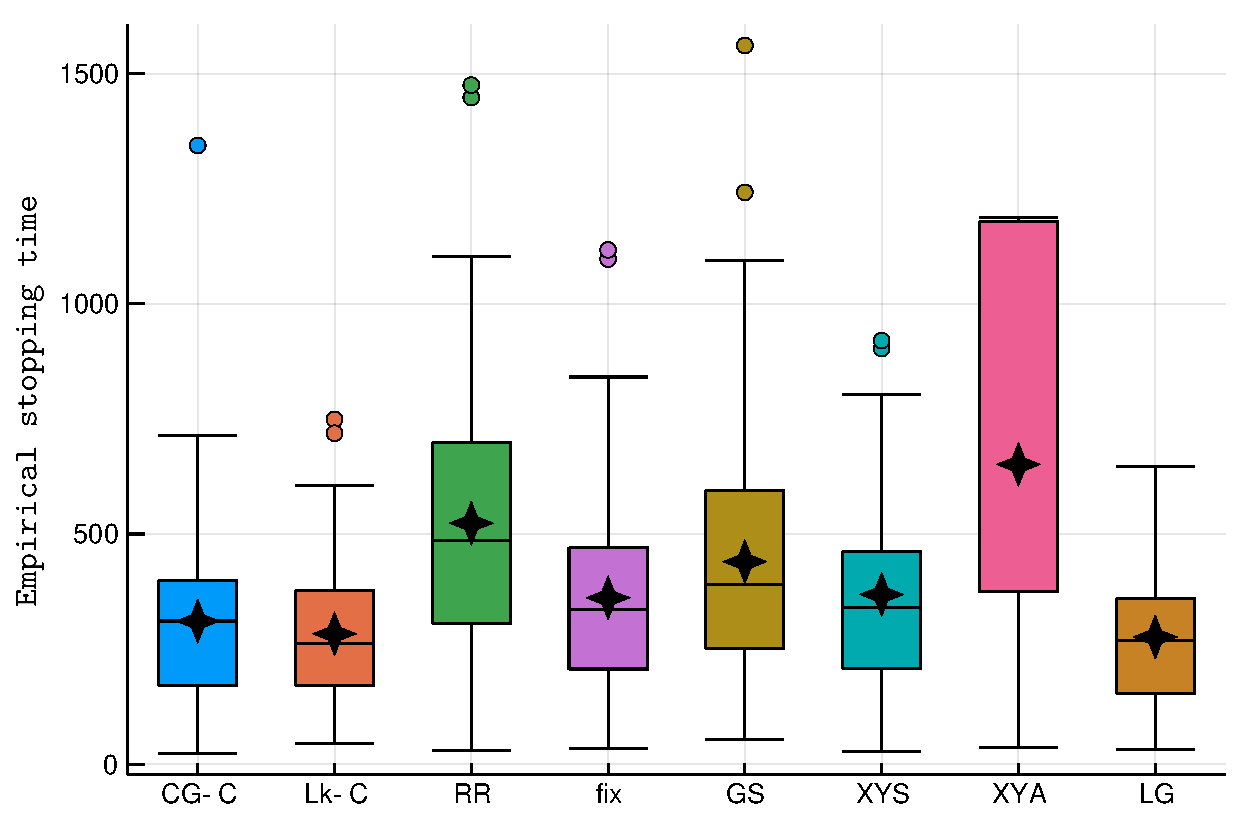
\includegraphics[clip, width= 0.33\textwidth]{Chapter4/img/bai_sin_0-01}
 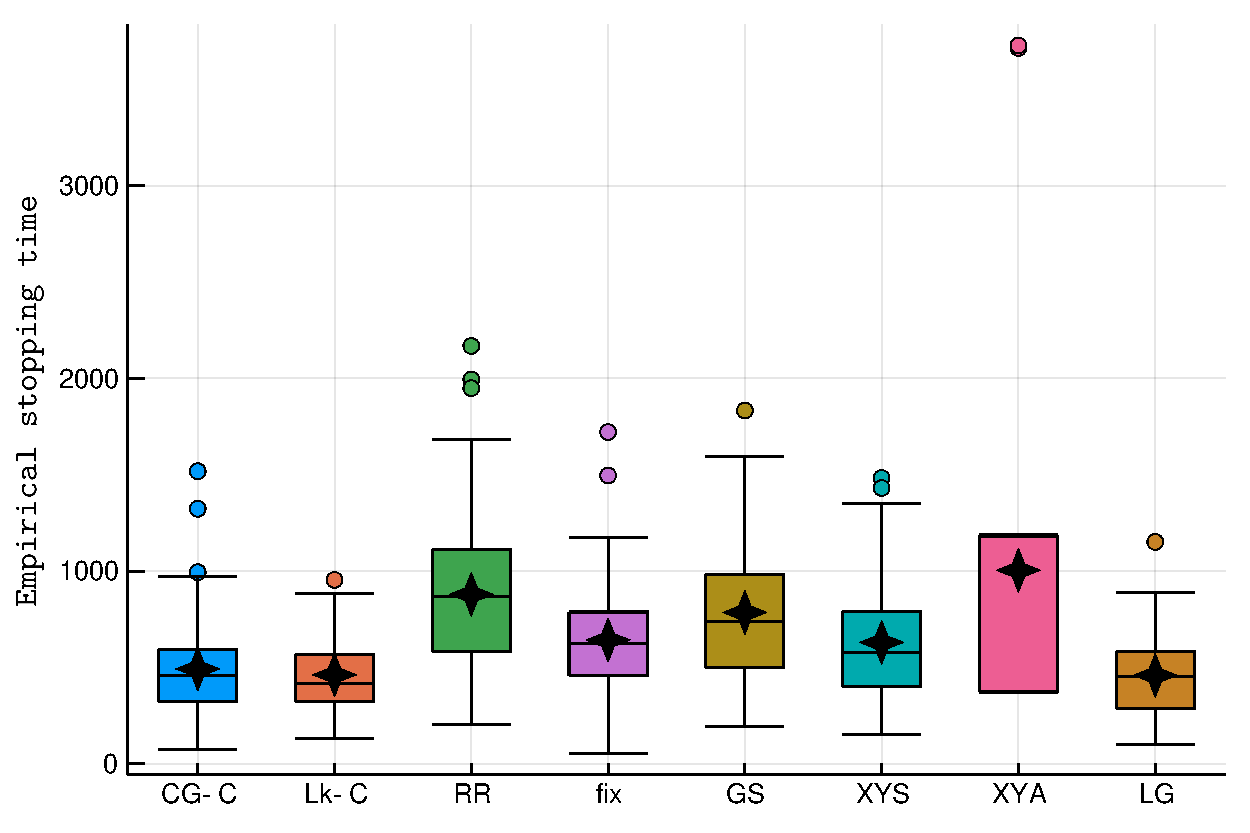
\includegraphics[clip, width= 0.33\textwidth]{Chapter4/img/bai_sin_0-0001}
 \caption{Sample complexity of different linear BAI sampling rules over the usual counter-example with $\delta=0.1, 0.01, 0.0001$ respectively. CG = \LGC,  Lk = \LG, RR = uniform sampling, fix = tracking the fixed weights, GS = \XYS with $\gopt$-allocation, XYS = \XYS with $\xyopt$-allocation, LG = \LGapE. The mean stopping time is represented by a black cross.}
 \label{fig:sample_complexity_1}
\end{figure}

For the second instance, we consider 20 arms randomly generated from the unit sphere $\mathbb{S}^{d-1}\eqdef\{a\in\R^d; \normm{a}_2=1\}$. We choose the two closest arms $a, a'$ and we set $\theta = a + 0.01(a'-a)$ so that a is the best arm. This setting has already been considered by~\citet{tao2018alba}. We report the same box plots over 100 replications as before with increasing dimension in Fig.~\ref{fig:sample_complexity_2}. More precisely, we set $d=6, 8, 10, 12$ respectively, and always keep a same $\delta = 0.01$. Our algorithms consistently show strong performances compared to other algorithms apart from \LGapE. Moreover, we can see that in these random examples, \LGC works better than the non-confexified one, and is even competitive compared to \LGapE.


\begin{figure}[ht]
 \centering
 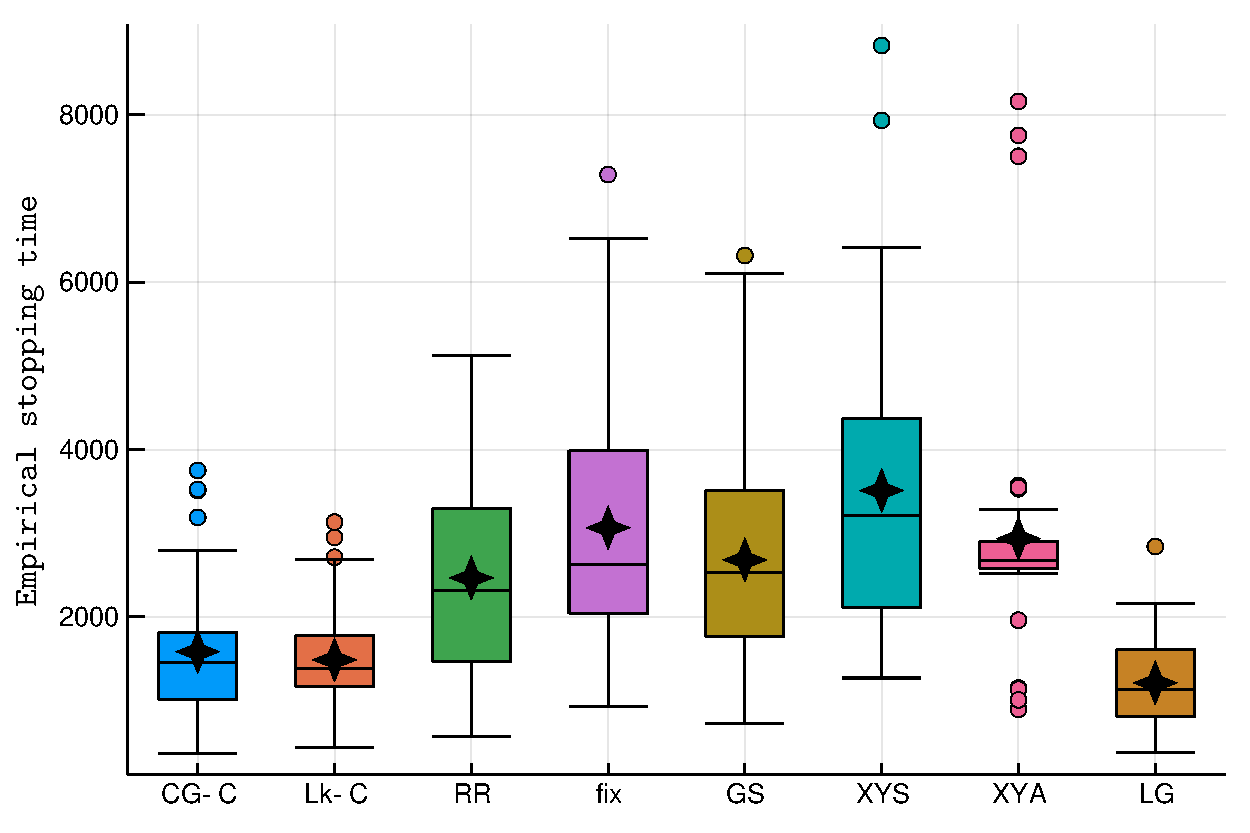
\includegraphics[clip, width= 0.33\textwidth]{Chapter4/img/bai_dim_6}
 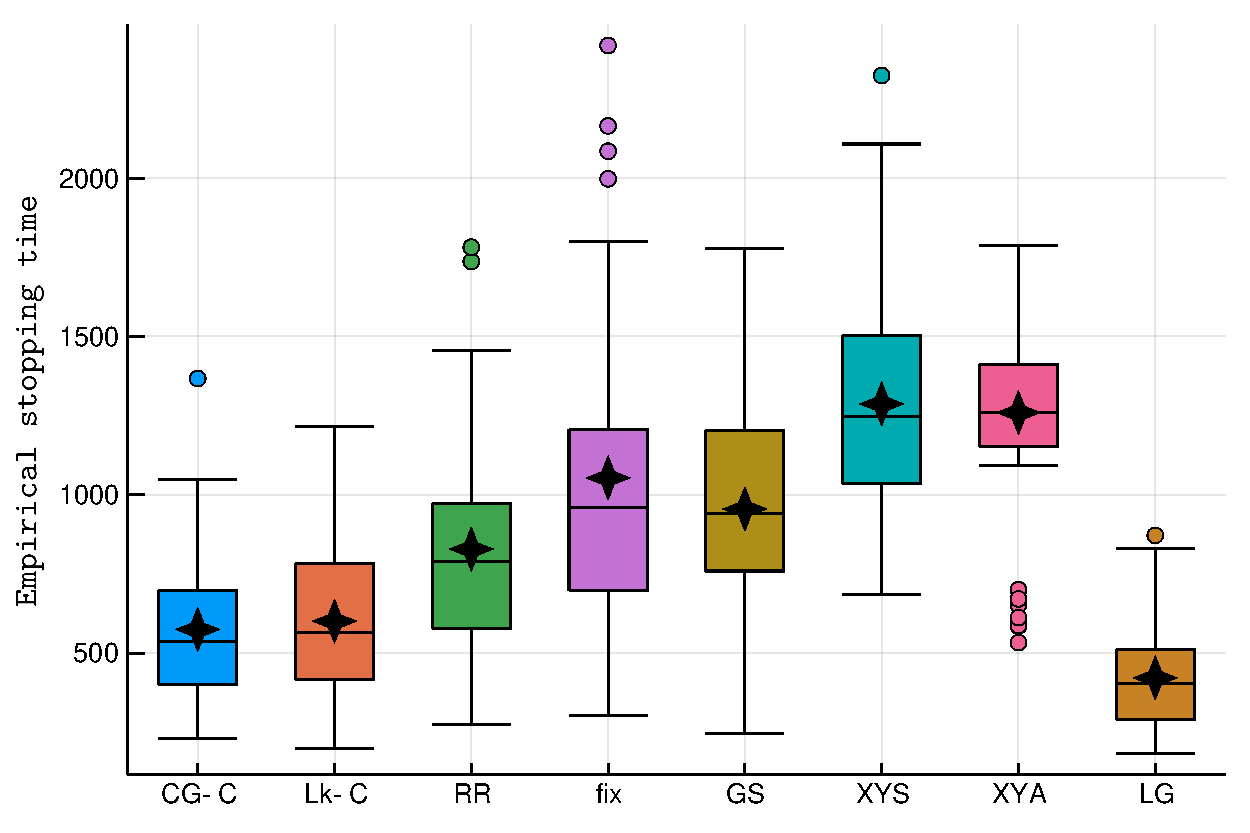
\includegraphics[clip, width= 0.33\textwidth]{Chapter4/img/bai_dim_8}
 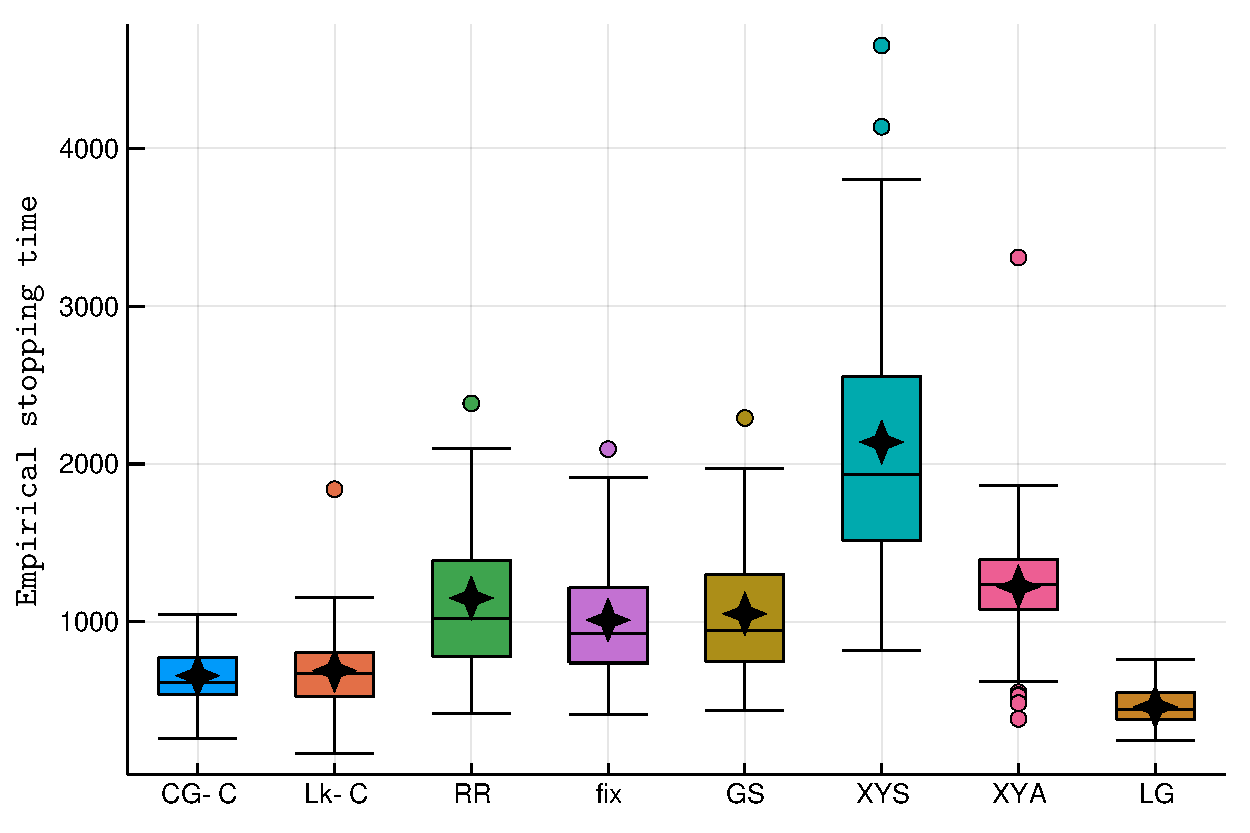
\includegraphics[clip, width= 0.33\textwidth]{Chapter4/img/bai_dim_10}
 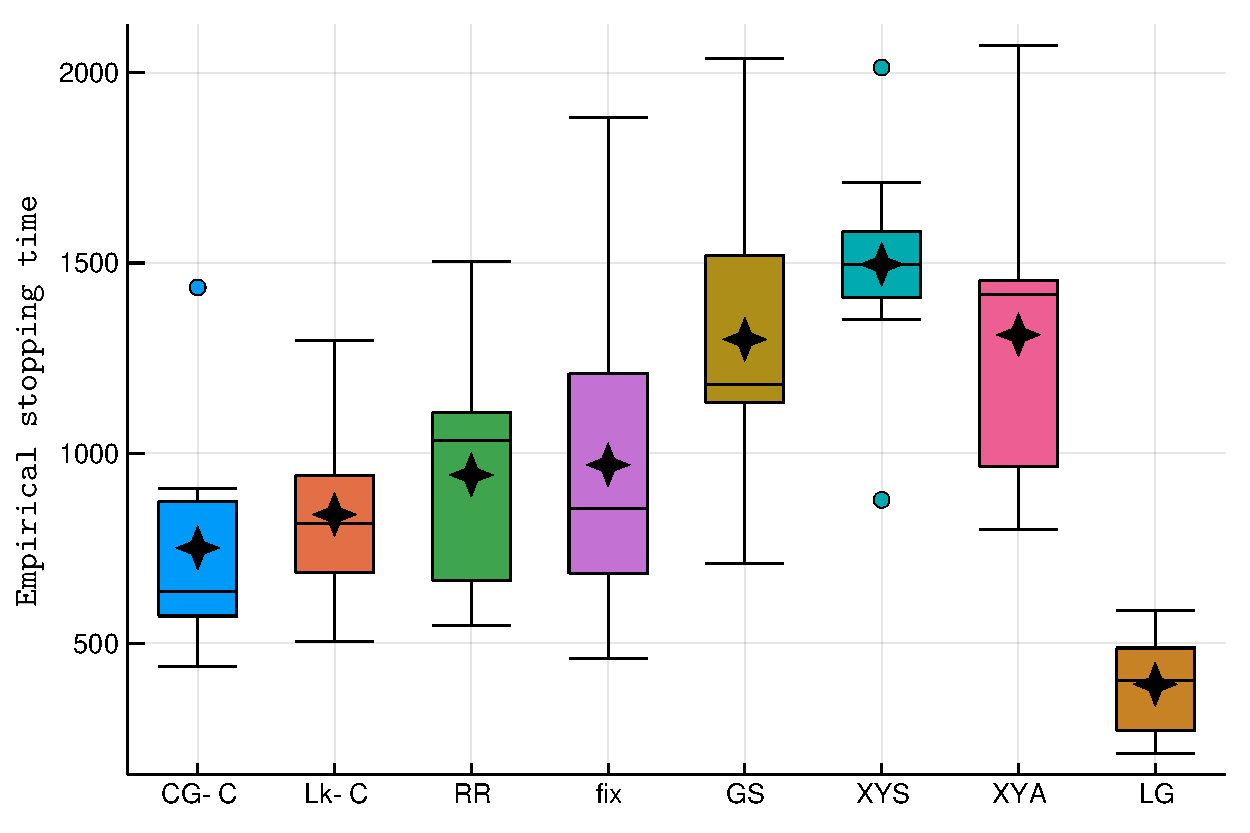
\includegraphics[clip, width= 0.34\textwidth]{Chapter4/img/bai_dim_12}
 \caption{Sample complexity of different linear BAI sampling rules over random unit sphere vectors with $d=6, 8, 10, 12$ from left to right.}
 \label{fig:sample_complexity_2}
\end{figure}

We stress that although the main focus of this chapter is theoretical, with algorithms that are asymptotically optimal, our methods are also competitive with earlier algorithms experimentally.


%!TEX root = ../Chapter4.tex
\section{Discussion}\label{sec:lgc.discussion}

In this chapter, we designed the first practically usable asymptotically optimal sampling rules for the pure exploration game for finite-arm linear bandits. Whether the boundedness assumption is necessary to obtain optimal algorithms remains an open question.

Note that since the publication of our work, several other asymptotically optimal algorithms have been proposed~\citep{zaki2020linear,jedra2020linear,katz-samuels2020practical}. Particularly, \cite{jedra2020linear} and \cite{katz-samuels2020practical} also study the fixed-budget setting for linear bandits BAI. Later, \cite{yang2021linear} propose a minimax optimal algorithm for fixed-budget BAI.

More generally, however, the part of fixed-confidence pure exploration algorithms that needs an improvement the most is the stopping rule. While the one we used guarantees $\delta$-correctness, it is very conservative. Indeed, the experimental error rates of algorithms using that stopping rule are orders of magnitude below $\delta$. This means that the concentration inequality does not reflect the query we seek to answer. It quantifies deviations of the $d$-dimensional estimate in all directions (morally, along $2^d$ directions). However, for the usual BAI setting with $d$ arms in an orthogonal basis, it would be sufficient to control the deviation of that estimator in $d-1$ directions to make sure that $i^*(\theta) = i^*(\hat{\theta}_t)$.

Finally, the good performance of \LGapE raises the natural question of whether it could be proven to have similar asymptotic optimality.

% \section{Discussion}\label{sec:conclusion}
%
% %\begin{itemize}
% %\item Fast rates for saddle point computation?
% %\item Changing arm sets? well defined? not clear.
% %\item exploration can be used as subroutine in a regret minimization algorithm
% %\end{itemize}
%
% \paragraph{Computational complexity} First note that the complexity of one step of \LG is $O( C(\text{stopping rule} +A))$ In BAI, the complexity of one step of \LGC (or \LG) is dominated by computing the best response for nature. Indeed, even in the unbounded case, it involves the inversion of a new matrix $V_{w_s^i}$
%
%
%
% \paragraph{Stopping rule} More generally, the aspect of fixed confidence pure exploration that needs an improvement the most is the stopping rule. While the one used here guarantees $\delta$-correctness, it is very conservative. Indeed, the experimental error rates of algorithms using that stopping rule are orders of magnitude below $\delta$. There are at least two ways to devise better stopping rules. First, the threshold $\beta(t,\delta)$ such that for all $t$, $\Vert \theta - \hat{\theta} \Vert^2_{V_{N_t}} \le \beta(t,\delta)$, could perhaps be made smaller. Second and most importantly, that concentration inequality does not reflect the query we seek to answer. It quantifies deviations of the $d$-dimensional estimate in all directions (morally, along $2^d$ directions). However, for the usual best-arm identification setting with $d$ arms in an orthogonal basis, it would be sufficient to control the deviation of that estimator in $d-1$ directions to be sure that $i^*(\theta) = i^*(\hat{\theta}_t)$.


% \newpage
% \bibliographystyle{plainnat}
% \bibliography{Major,manual_bib}
% \newpage

\begin{subappendices}
\addtocontents{toc}{\protect\setcounter{tocdepth}{0}}
%!TEX root = ../Chapter3.tex
\section{Outline}\label{app:lgc.outline}

The appendices are organized as follows:
\begin{itemize}[label=$\square$]
    \item Notation is given in Appendix~\ref{app:lgc.notations}. 
    \item We give a full proof of Theorem~\ref{th:lb_genral} in Appendix~\ref{app:lgc.lower_bound}.
    \item We list and elaborate in detail several pure exploration problems in Appendix~\ref{app:lgc.examples}.
    \item Appendix~\ref{app:lgc.proof} is dedicated to the proof of sample complexity for the convexified algorithm \LGC.
    \item Appendix~\ref{app:lgc.proof_nc} is dedicated to the proof of sample complexity for the non-convexified algorithm \LG.
    \item Appendix~\ref{app:lgc.concentration} is dedicated to some important concentration results.
    \item We discuss the tracking procedure in Appendix~\ref{app:lgc.tracking}.
    \item We discuss the stopping rules in Appendix~\ref{app:lgc.stopping}.
    \item Finally, we provide some further details about the experiments in Appendix~\ref{app:lgc.implem}.
\end{itemize}


%!TEX root = ../Chapter3.tex
\section{Notation}\label{app:lgc.notations}

\begin{table}[ht]
	\centering
	\caption{Table of notation for Chapter~\ref{chap:lgc}.}
	\begin{tabular}{@{}l|l@{}}
		\toprule
		\thead{Notation} & \thead{Meaning} \\ \midrule
		$\cM$ & set of parameters \\
        $M$ & upper bound on the norm of $\theta$\\
		$\cA$ & finite set or arms  \\
        $A$ & number of arms \\
        $\cB$ & transductive set \\
        $B$ & number of elements in the transductive set \\
        $\cI$ & finite set of answers \\
        $I$ & number of answers \\
        $L$ & upper bound on the norms of the arms\\
        $\theta$ & parameter in $\cM$ \\
        $a_t$ & arm pulled at time $t$ \\
        $N_t^a = \sum_{s=1}^t \ind_{\{a_s = a\}}$ & number of draws of arm $a$ at time $t$\\
        $N_t =(N_t^a)_{a\in\cA}$ & vector of number of draws\\
        $N_t^{a,i} = \sum_{s=1}^t \ind_{\{a_s = a, i_t = i\}}$ & number of draws of arm $a$ for a given answer $i$\\
        $\eta$ & regularization parameter\\
        $\htheta_t$ & regularized least square estimate\\
		\bottomrule
	\end{tabular}
\end{table}


%%!TEX root = ../Chapter3.tex
\section{Proofs of the Lower Bounds and Equivalent Formulations}\label{app:lgc.lower_bound}

We start this section by proving the lower bound.

\begin{proof}[Proof of Theorem~\ref{th:lb_genral}]
Fix $\lambda\in\neg\istar(\theta)$ in the alternative of $\theta$. Thanks to the contraction of the entropy and the chain rule (see \citealt{garivier2018explore}), we have

\[
\kl\!\big(\P_\theta(\hi = \istar),\P_\lambda(\hi = \istar)\big) \leq \sum_{a\in\cA} \E_\theta\big[N_a(\tau_\delta)\big]\frac{\normm{\theta -\lambda^i}_{a a^\top}^2}{2}\,,
\]
where we denote by $\kl(p,q)$ the Kullback-Leibler divergence between two Bernoulli distributions $\Ber(p)$ and $\Ber(q)$
\[
\kl(p,q) = p \log\!\left(\frac{p}{q}\right) + (1-p) \log\!\left(\frac{1-p}{1-q}\right)\,.
\]
Since the algorithm is $\delta$-correct we know that
\[
\P_\lambda\big(\hi = \istar(\theta)\big) \leq \delta \leq \frac{1}{2} \leq  1-\delta \leq \P_\theta\big(\hi = \istar(\theta)\big)\,.
\]
Thanks to monotonic properties of the function $\kl(\cdot,\cdot)$ and the inequality $\kl(1-p,p) \geq -\log(2.4p)$, see \citet{garivier2018explore}, it yields
\[
\kl\big(\P_\theta(\hi = \istar(\theta)),\P_\lambda(\hi = \istar(\theta))\big) \geq \kl(1-\delta,\delta) \geq \log\left(\frac{1}{2.4\delta}\right)\,,
\]
thus
\[
\log\left(\frac{1}{2.4\delta}\right) \leq \sum_{a\in\cA} \E_\theta\big[N_a(\tau_\delta)\big]\frac{\normm{\theta -\lambda^i}_{a a^\top}^2}{2}\,.
\]
Using the previous inequality is true for all $\lambda\in\neg\istar(\theta)$ and that the vector of components $\E_\theta\big[N_a(\tau_\delta)\big]/\E_\theta\big[\tau_\delta\big]$ belongs to the probability simplex $\Sigma_A$ we get
\begin{align*}
\log\left(\frac{1}{2.4\delta}\right) &\leq \E_\theta[\tau_\delta] \inf_{\lambda\in\neg \istar(\theta)} \sum_{a=1}^K \frac{\E_\theta\big[N_a(\tau_\delta)\big]}{\E_\theta[\tau_\delta]}\frac{\normm{\theta -\lambda^i}_{a a^\top}^2}{2}\\ &\leq \E_\theta[\tau_\delta] \sup_{w\in\Sigma_K}
\inf_{\lambda\in\neg \istar(\theta)} \sum_{a=1}^K w_a\frac{\normm{\theta -\lambda^i}_{a a^\top}^2}{2}\,.
\end{align*}
Dividing the previous inequality by $\log(1/\delta)$ and taking the limit inferior when $\delta$ goes to zero allows us to conclude.
\end{proof}

We restate and prove below Lemma~\ref{lem:sion_convexify}.
\begin{lemma}
  \label{lem:sion_convexify_extended} For all $\theta \in\cM$,
\begin{align}
  \Tstar(\theta)^{-1} &= \max_{i\in \cI} \max_{w \in \Sigma_A} \inf_{\lambda\in \neg i} \frac{\normm{\theta - \lambda}_{V_w}^2}{2}\label{eq:sion_base}\\
  &=\max_{\tw \in \Sigma_{AI}} \inf_{\tlambda\in \prod_i (\neg i) }\frac{1}{2} \sum_{(a,i)\in\cA\times\cI}\tw^{a,i}\normm{\theta - \lambda^i}_{aa^\top}^2\label{eq:sion_nature_first}\\
  & = \max_{\tw \in \Sigma_{AI}}\inf_{\tq\in \prod_i\cP(\neg i) }\!\sum_{(a,i)\in\cA\times\cI}\!\!\!\tw^{a,i}\E_{\lambda^i\sim \tq^i}\normm{\theta - \lambda^i}_{aa^\top}^2 \label{eq:sion_both}\\
  &= \inf_{\tq\in \prod_i\cP(\neg i) } \frac{1}{2}\max_{(a,i)\in\cA\times\cB}\E_{\lambda^i\sim \tq^i}\normm{\theta - \lambda^i}_{aa^\top}^2\label{eq:sion_player_fisrt}\,.
\end{align}

\end{lemma}
\begin{proof}
  To go from \eqref{eq:sion_nature_first} to \eqref{eq:sion_both} just use the fact that the second player can use indifferently mixed or pure strategy. The equality between \eqref{eq:sion_both} and \eqref{eq:sion_player_fisrt} is just an application of the Sion lemma (see \citealt{degenne2019pure}).
  It remains to prove \eqref{eq:sion_nature_first}. First note that we can replace the first maximum in \eqref{eq:sion_base} over $\istar(\theta)$ by a maximum over $\cI$ because when $i\notin \istar(\theta)$ we know that $\theta\in \neg i$. Since we can express the maximum over the answers as a maximum over the probability simplex $\Sigma_I$ we have
\begin{align*}
    \max_{i\in \cI} \sup_{w \in \Sigma_A} \inf_{\lambda\in \neg i} \frac{1}{2}\sum_{a\in\cA} w_a \normm{\theta - \lambda}_{aa^\top}^2 &= \max_{\rho \in \Sigma_I} \sum_{i\in\cI}\sup_{w \in \Sigma_A} \inf_{\lambda\in \neg i} \frac{1}{2}\sum_{a\in\cA} \rho_i w_a\normm{\theta - \lambda}_{aa^\top}^2\\
     &= \max_{\rho\in \Sigma_I} \sum_{i\in \cI} \sup_{w^i \in \Sigma_A} \inf_{\lambda^i\in \neg i}\frac{1}{2} \sum_{a\in\cA} \rho_i w_a^i\normm{\theta - \lambda^i}_{aa^\top}^2\\
     &= \sup_{\tw \in \Sigma_{A I}} \inf_{\tlambda \in \prod_{i\in\cI}\neg i} \frac{1}{2}\sum_{(a,i)\in \cA\times\cI}  \tw_a^i \normm{\theta - \tlambda^i}_{aa^\top}^2\,,
\end{align*}
 where in the last line we used that all $\tw \in \Sigma_{A I}$ can be written $\tw_a^i = \rho_i w_a^i $ with $\rho \in \Sigma_I$ and $w^i \in \Sigma_A$ for all $i \in \cI$.
\end{proof}


%!TEX root = ../Chapter4.tex
\section{Examples}\label{app:lgc.examples}

We gather in this appendix several pure exploration problems for linear bandits. We first state a useful lemma.

\begin{lemma}\label{lem:lagrange_alternative}
For $\theta, \lambda \in \R^d\,$, $w$ in the interior of the probability simplex $\interior{\Sigma_A}$, $y\in\R^d\,$, $x\in\R$, we have
\begin{align*}
\inf_{\lambda:\ \langle \lambda,y\rangle \geq x} \frac{\normm{\theta-\lambda}^2_{V_w}}{2} = \begin{cases}
\dfrac{(x - \langle\theta,y\rangle)^2}{2 \normm{y}_{V_w^{-1}}^2} &\text{if } x \geq \langle\theta,y\rangle \\
0 &\text{otherwise}
\end{cases}\,.
\end{align*}
\end{lemma}

\begin{proof}
We consider the Lagrangian of the problem, and we obtain
\begin{align*}
  \inf_{\lambda:\ \langle \lambda,y \rangle \geq x} \frac{\normm{\theta-\lambda}^2_{V_w}}{2}
  &= \sup_{\alpha \geq 0}\inf_{\lambda \in \R^d} \frac{\normm{\theta-\lambda}^2_{V_w}}{2}+ \alpha (x-\langle\lambda,y\rangle)\\
  &=  \sup_{\alpha \geq 0} \alpha (x-\langle\theta,y\rangle) - \alpha^2 \frac{\normm{y}^2_{V_w^{-1}}}{2}\\
  &= \begin{cases}
  \dfrac{(x - \langle\lambda,y\rangle)^2}{2 \normm{y}_{V_w^{-1}}^2} &\text{if } x \geq \langle\theta,y\rangle \\
  0 & \text{otherwise}
  \end{cases}\,,
\end{align*}
where the infimum in the first equality is reached at $\lambda = \theta + \alpha V_w^{-1} y$ and the supremum in the last equality is reached at $\alpha = (x- \langle\theta,y\rangle)/\normm{y}_{V_w^{-1}}^2$ if $x \geq \langle\theta,y\rangle$ and at $\alpha = 0$ else.
\end{proof}

\subsection{Best-arm identification}
\label{app:bai}
For BAI the goal is to identify the arm with the largest mean. Thus, the set of parameters is $\cM=\cR^d/\{\theta\in\R^d:\  |\argmax_{a\in\cA} \langle\theta,a\rangle|>1\}$, the set of possible answers is $\cI = \cA$ and the correct answer is given by $\istar(\theta)=\astar(\theta)\eqdef \argmax_{a\in\cA} \langle\theta,a\rangle$.
\begin{lemma}
\label{lem:complexity_bai}
For all $\theta\in \cM$,
\[
\Tstar(\theta)^{-1} = \max_{w\in\Sigma_A} \min_{a\neq \astar(\theta)} \frac{\big\langle \theta, \astar(\theta)-a\big\rangle^2}{2 \normm{\astar(\theta)-a}_{V_w^{-1}}^2}\,,
\]
and
\[
\Tstar(\theta) = \min_{w\in\Sigma_A} \max_{a\neq \astar(\theta)} \frac{2\normm{\astar(\theta)-a}_{V_w^{-1}}^2}{\big\langle \theta, \astar(\theta)-a\big\rangle^2}\,.
\]
\end{lemma}
\begin{proof}
Recall that the characteristic time is given by
\[
\Tstar(\theta)^{-1} = \max_{w \in \Delta_A} \inf_{\lambda\in \neg \astar(\theta)} \frac{\normm{\theta - \lambda}_{V_w}^2}{2}\,.
\]
We just express the set $\neg \astar(\theta)$ as a union of convex sets, and then compute the infimum for each one of them. Using Lemma~\ref{lem:lagrange_alternative}, it yields
\begin{align*}
  \Tstar(\theta)^{-1} &= \max_{w \in \Delta_A} \min_{a \neq \astar(\theta)} \inf_{\lambda: \langle\lambda,a\rangle > \langle\lambda,\astar(\theta)\rangle} \frac{\normm{\theta - \lambda}_{V_w}^2}{2}\\
  &= \max_{w \in \Delta_A} \min_{a \neq \astar(\theta)} \frac{\big\langle \theta, \astar(\theta)-a\big\rangle^2}{2 \normm{\astar(\theta)-a}_{V_w^{-1}}^2}\,.
\end{align*}
The formula for $\Tstar(\theta)$ is then straightforward given the one for  $\Tstar(\theta)^{-1}$.

\end{proof}
In fact the characteristic time is just a particular case of the optimal transductive design. Indeed if we set
\[
\cBstar(\theta) \eqdef \left\{ \frac{1}{\left|\big\langle \theta, \astar(\theta)-a\big\rangle\right|}\big(\astar(\theta)- a\big): a\in\cA/\big\{\astar(\theta)\big\}  \right\}\,,
\]
then we have $\Tstar(\theta) = 2 \cA\cBstar(\theta)$ where
\[
\cA\cBstar(\theta) \eqdef  \min_{w\in\Sigma_A} \max_{b\in \cBstar} \normm{b}_{V_w^{-1}}^2\,.
\]

\paragraph{Best response.} There is an explicit formula for the best response in BAI. Indeed if we inspect the proof of Lemma~\ref{lem:complexity_bai} we have
\[
\inf_{\lambda\in \neg \astar(\theta)} \frac{\normm{\theta - \lambda}_{V_w}^2}{2} = \min_{a \neq \astar(\theta)} \normm{\theta-\lambda^\star_a}_{V_w^{-1}}\,.
\]
where $\lambda^\star_a$ is defined in Lemma~\ref{lem:best_response_BAI}.

\begin{lemma}
\label{lem:best_response_BAI}
For $\theta \in\R^d\,$, $w$ in the interior of the probability simplex $\interior{\Sigma_A}$, we have
\[
\min_{\substack{\langle \lambda,a-\astar(\theta)\rangle\geq 0}} \normm{\theta -\lambda }_{V_w}^2 = \frac{\big\langle \theta, \astar(\theta)-a\big\rangle^2}{2 \normm{\astar(\theta)-a}_{V_w^{-1}}^2}\,,
\]
and $\lambda^\star_a$ defined below attains the infimum of the left hand term above
\[
\lambda^\star_a = \theta - \frac{\max\left(\langle \theta, \astar(\theta)-a\rangle,0\right)}{\normm{\astar(\theta)-a}^2_{(V_w+\gamma I_d)^{-1}}} V_w^{-1}(a^\star - a)\,.
\]
\end{lemma}
\begin{proof}
See proof of Lemma~\ref{lem:lagrange_alternative}.
\end{proof}


\subsubsection{Bounded BAI}
\label{app:bounded_bai}
One straightforward extension of this setting is to consider the \emph{bounded} BAI. In this case, the set of parameters is $\cM=\{\theta \in \R^d:\ |\argmax_{a\in\cA} \langle\theta,a\rangle|=1 \text{ and } \normm{\theta}\leq M\}$ for some $M>0$. The set of possible answers is $\cI = \cA$ and the correct answer is given by $\istar(\theta)=\astar(\theta)\eqdef \argmax_{a\in\cA} \langle\theta,a\rangle$.
This additional assumption reduces the characteristic time to
\[
\Tstar(\theta)^{-1} = \max_{w\in\Sigma_A} \min_{a\neq \astar(\theta)} \inf_{\substack{\langle \lambda,a-\astar(\theta)\rangle>0\\ \normm{\lambda}\leq M}} \normm{\theta -\lambda }_{V_w}^2 \,.
\]
But the best response is less trivial to compute, in particular there is no closed formula for $\lambda^\star_a$ as in BAI, see Lemma~\ref{lem:lagrange_bounded_BAI}.
\begin{lemma}
  \label{lem:lagrange_bounded_BAI}
For $\theta, \lambda \in \R^d\,$, $w$ in the interior of the probability simplex $\interior{\Sigma_A}$,
\begin{align}\label{eq:bounded_bai}
\min_{\substack{\langle \lambda,a-\astar(\theta)\rangle\geq 0\\ \normm{\lambda}\leq M}} \normm{\theta -\lambda }_{V_w}^2 = \sup_{\gamma\geq 0} \frac{\max\left(\langle \theta, (V_w+\gamma I_d)^{-1} V_w (\astar(\theta)-a)\rangle,0\right)^2 }{2\normm{\astar(\theta)-a}^2_{(V_w+\gamma I_d)^{-1}}}- \frac{\gamma}{2}\left(\normm{\theta}^2-M^2\right)\,.
\end{align}
And if $\gamma$ attains the supremum in the right hand term of~\eqref{eq:bounded_bai}, then
\[
\lambda = \theta - \frac{\max\left(\langle \theta, (V_w+\gamma I_d)^{-1} V_w (\astar(\theta)-a)\rangle,0\right)}{\normm{\astar(\theta)-a}^2_{(V_w+\gamma I_d)^{-1}}} (V_w+\gamma I_d)^{-1}(a^\star - a)\,,
\]
attains the minimum of the left hand term of~\eqref{eq:bounded_bai}.
\end{lemma}
\begin{proof}
We set $\astar(\theta) = \astar$, and introduce the Lagrangian
\[
 \inf_{\substack{\langle \lambda,a-\astar \rangle>0\\ \normm{\lambda}\leq M}} \normm{\theta -\lambda }_{V_w}^2 = \sup_{\gamma\geq 0, \alpha\geq 0} \inf_{\substack{\langle \lambda,a-\astar\rangle>0\\ \normm{\lambda}\leq M}} \normm{\theta -\lambda }_{V_w}^2 +\alpha \langle \theta, \astar-a\rangle + \frac{\gamma}{2}\left(\normm{\lambda}^2-M^2 \right)\,.
\]
The infimum above is attained for
\[
\lambda = \theta - \alpha (V_w + \gamma I_d)^{-1}(\astar-a)\,.
\]
Thus the Lagrangian reduces to
\[
\inf_{\substack{\langle \lambda,a-\astar \rangle>0\\ \normm{\lambda}\leq M}} \normm{\theta -\lambda }_{V_w}^2 = \sup_{\gamma\geq 0, \alpha\geq 0}
-\frac{\alpha^2}{2} \normm{\astar-a}^2_{V_w+\gamma I_d} + \alpha \langle \theta, (V_w+\gamma I_d)^{-1}V_w (\astar-a)\rangle +\frac{\gamma}{2}\left(\normm{\theta}^2-M^2 \right)\,.
\]
The supremum in $\alpha$ is reached for
\[
\alpha =\frac{\max\left(\langle \theta, (V_w+\gamma I_d)^{-1} V_w (\astar-a)\rangle,0\right)}{\normm{\astar-a}^2_{(V_w+\gamma I_d)^{-1}}}\,.
\]
Using this particular $\alpha$ in the definition of $\lambda$ and in the Lagrangian allows us to conclude.
\end{proof}

\subsubsection{Transductive BAI}

We can also consider the transductive BAI~\citep{fiez2019transductive} where the agent wants to find the best arm of a different set $\cB$ that the one he is allow to pull. Precisely the set of parameters is $\cM=\cR^d/\{\theta\in\R^d:\  |\argmax_{b\in\cB} \langle\theta,b\rangle|>1\}$, the set of possible answers is $\cI = \cB$ and the correct answer is given by $\istar(\theta)=\bstar(\theta)\eqdef \argmax_{b\in\cB} \langle\theta,b\rangle$.

The characteristic time in this case is
\[
\Tstar(\theta)^{-1} = \max_{w\in\Sigma_A} \min_{b\neq \bstar(\theta)} \frac{\big\langle \theta, \bstar(\theta)-b\big\rangle^2}{2 \normm{\bstar(\theta)-b}_{V_w^{-1}}^2}\,.
\]
Note that the dependency on the arm set $\cA$ here only appears through the matrix $V_w$.


% \subsection{Threshold bandits}
% \label{app:threshold_bandits}
% In this example the goal is to identify the set of arms whose mean is above a threshold $\iota\in \R$ known by the agent. Thus, the set of parameters is $\cM=\cR^d/\{\theta\in\R^d:\ \exists a\in \cA,\, \langle \theta,a\rangle = \iota\}$, the set of possible answers is $\cI = \cP(\cA)$, the power set of the set of arms and the correct answer is given by $\istar(\theta)=\{a\in\cA:\ \langle \theta,a\rangle \geq \iota\}$.
% We can also express in this example the characteristic time in a more explicit way.
% \begin{lemma}
% \label{lem:complexity_threshold_bandits}
% For all $\theta\in \cM$,
% \[
% \Tstar(\theta)^{-1} =  \max_{w\in\Sigma_A} \min_{a\in\cA} \frac{\big(\iota -\langle \theta,a\rangle\big)^2}{2 \normm{a}_{V_w^{-1}}^2}\,,
% \]
% and $\Tstar(\theta)= 2\cA\cA(\iota)$, where we define $\cA(\iota)\eqdef \{ |\iota- \langle\theta,a\rangle|^{-1} a:\ a\in\cA\}$ and
% \[
% \cA\cA(\iota) \eqdef  \min_{w\in\Sigma_A} \max_{a\in\cA(\iota)}\normm{a}_{V_w^{-1}}^2\,.
% \]
% \end{lemma}
% \begin{proof}
% We proceed as the proof of Lemma~\ref{lem:complexity_bai}. We have, using Lemma~\ref{lem:lagrange_alternative},
% \begin{align*}
%   \Tstar(\theta)^{-1} &= \max_{w \in \Delta_A} \min_{a\in\cA} \inf_{\lambda:\ \text{sign}(\iota-\langle\lambda,a\rangle)\langle\lambda,a\rangle > \iota} \frac{\normm{\theta - \lambda}_{V_w}^2}{2}\\
%   &= \max_{w \in \Delta_A} \min_{a\in\cA}  \frac{\big(\iota -\langle \theta,a\rangle\big)^2}{2 \normm{a}_{V_w^{-1}}^2}\,.
% \end{align*}
% \end{proof}
% Note that we recover in this example a weighted version of the G-complexity ($\gopt$-complexity) defined in Section~\ref{sec:lower_bound}. In particular if $\theta=0$ and $\iota=1$ then
% \[
% \Tstar(\theta) =2\gopt = 2d\,.
% \]
% That makes sense since in this case, one shall estimate \emph{uniformly} the mean of each arms.


% \subsubsection{Transductive threshold bandits}
% \label{app:transductive_threshold_bandits}
% We can generalize the previous example to any set of arms. Indeed if we fix a finite set of vector $\cB\in\R^d$ the goal is then to identify all the elements $b$ of this set such that $\langle \theta, b \rangle \geq \iota$ for a known threshold $\tau \in \R$. Thus, the set of parameters is $\cM=\cR^d/\{\theta\in\R^d:\ \exists b\in \cB,\, \langle \theta,b\rangle = \iota\}$, the set of possible answers is $\cI = \cP(\cB)$ and the correct answer is given by
% $\istar(\theta)=\{b\in\cB:\ \langle \theta,b\rangle \geq \iota\}$. The characteristic time makes appear, unsurprisingly, in this case, the transductive optimal design \citep{yu2006active}.
% \begin{lemma} For all $\theta \in\cM$,
%   \label{lem:complexity_transductive_threshold_bandits}
%   \[
%   \Tstar(\theta)^{-1} =  \max_{w\in\Sigma_A} \min_{b\in\cB} \frac{\big(\iota -\langle \theta,b\rangle\big)^2}{2 \normm{b}_{V_w^{-1}}^2}\,,
%   \]
%   and $\Tstar(\theta)= 2\cA\cB(\iota)$, where we defined $\cB(\iota)\eqdef \{ |\iota- \langle\theta,b\rangle|^{-1} b:\ b\in\cB\}$ and
%   \[
%   \cA\cB(\iota) \eqdef  \min_{w\in\Sigma_A} \max_{b\in\cB(\iota)}\normm{b}_{V_w^{-1}}^2\,.
%   \]
% \end{lemma}
% \begin{proof}
%   Simple adaptation of the proof of Lemma~\ref{lem:complexity_threshold_bandits}.
% \end{proof}
% Again, in particular, if $\theta=0$ and $\tau=1$ we recover the complexity of the optimal transductive design
% \[
% \Tstar(\theta)^{-1} = 2 \cA\cB\,.
% \]


%%!TEX root = ../Chapter3.tex
\section{Oracle Computations}

\paragraph{Best response.}

Let $x_\mu \in \mathcal A$ be the best action for $\mu$ and $y\in \mathcal A$ different from $x$.
\begin{align*}
\argmin_{\lambda:(y-x_\mu)^\top\lambda \ge 0}\frac{1}{2} \sum_{a \in \mathcal A} w^a (\mu - \lambda)^2_{aa^\top}
&= \mu - \frac{(y-x_\mu)^\top \mu}{\Vert y-x_\mu \Vert^2_{V_w^{-1}}} V_w^{-1}(y - x)
\\
\min_{(y-x_\mu)^\top\lambda \ge 0}\frac{1}{2} \sum_{a \in \mathcal A} w^a (\mu - \lambda)^2_{aa^\top}
&= \frac{1}{2} \frac{((y-x_\mu)^\top \mu)^2}{\Vert y-x_\mu \Vert^2_{V_w^{-1}}}
\end{align*}

\paragraph{Oracle weights.}

The oracle weights are solution of the following problem:
\[
\argmax_{w \in \triangle_K} \min_{y \in \mathcal A} \frac{\Vert y-x_\mu \Vert^2_{\mu \mu^\top}}{\Vert y-x_\mu \Vert^2_{V_w^{-1}}} \quad \text{or equivalently} \quad \argmin_{w \in \triangle_K} \max_{y \in \mathcal A} \frac{\Vert y-x_\mu \Vert^2_{V_w^{-1}}}{\Vert y-x_\mu \Vert^2_{\mu \mu^\top}}
\]
The value of that problem at the optimum is
\[
\max_{w \in \triangle_K} \min_{y \in \mathcal A} \frac{1}{2}\frac{\Vert y-x_\mu \Vert^2_{\mu \mu^\top}}{\Vert y-x_\mu \Vert^2_{V_w^{-1}}}
= \frac{1}{2}\left(\min_{w \in \triangle_K} \max_{y \in \mathcal A} \frac{\Vert y-x_\mu \Vert^2_{V_w^{-1}}}{\Vert y-x_\mu \Vert^2_{\mu \mu^\top}}\right)^{-1}
= \frac{1}{2}H_{LB}^{-1}
\]
where $H_{LB}$ is the complexity defined by~\citet{soare2014linear}.

\paragraph{G-Allocation.}
 
 The G-allocation is defined by~\citet{soare2014linear} as the solution in $w$ of
 \[
\min_{w \in \triangle_K} \max_{x \in \mathcal A} \Vert x \Vert^2_{V_w^{-1}}
 \]

\paragraph{$\mathcal X \mathcal Y$-allocation.}

The $\mathcal X \mathcal Y$-allocation is defined by~\citet{soare2014linear} as the solution in $w$ of
 \[
\min_{w \in \triangle_K} \max_{y,x \in \mathcal A} \Vert y-x \Vert^2_{V_w^{-1}}
 \]

\paragraph{UCB computations.}

\begin{align*}
\left\{\begin{array}{ll}
\sup_\xi \quad &  \frac{1}{2} ((\xi - \lambda)^\top a)^2
\\
\text{s.t.} \quad & \frac{1}{2} \Vert \theta - \xi \Vert^2_V \le \alpha 
\end{array}\right.
&= \max_\pm\frac{1}{2} \left( (\theta - \lambda)^\top a \pm \sqrt{2 \alpha a^\top V^{-1} a} \right)^2
\end{align*}


%%!TEX root = ../Chapter3.tex
\section{Proof for the Sample Complexity: Convexified Algorithm}\label{app:lgc.proof}

In this section we prove the asymptotic optimality of \LGC.
\subsection{Events}\label{app:proof.events}
We fix a constant $\alpha>2$ and define the event where the least square estimator is concentrated around the true parameter,
\[
\cE_t = \left\{\forall s \leq  t:\ \frac{1}{2}\normm{\htheta_s-\theta}^2_{V_{N_s}+\eta I_d} \leq h(t)\eqdef \beta(t,1/t^\alpha)\right\}\,.
\]
This event holds with high probability
\begin{lemma}
\label{lem:prb_Et}
For all $t \geq 1$
\[
\P_\theta\left(\cE_t^c\right)\leq \frac{1}{t^{\alpha-1}}\,.
\]
\end{lemma}

\paragraph{Optimistic loss} We need to build an upper confidence bound for all $w\in\Sigma_{AI}$ on the true gain at time $s$
\[
g_{s}^{\theta}(w) = \frac{1}{2} \sum_{(a,i)\in\cA\times\cI} w^{a,i} \normm{\theta - \lambda_t^i}_{V_{w}}^2\,.
\]
For that, we just build confidence bound for each terms that appear in the right hand sum.
\begin{lemma}
\label{lem:confidence_bound_general}
On the event $\cE_t$, for all $a\in\cA\times\cI$ and $\lambda\in\cM$, for all $s\leq t$,
\[
\normm{\theta-\lambda}^2_{aa^\top} \leq \min\left(\max_\pm \left( \langle \htheta_{s} - \lambda,a\rangle \pm \sqrt{2 h(t)} \normm{a}_{(V_{N_s}+ \eta I_d)^{-1}} \right)^2,4L^2 M^2\right)
\]
\end{lemma}
\begin{proof}
First, note that since $\theta,\lambda\in\cM$ their norms is bounded by $M$, thus it holds
\[
\normm{\theta-\lambda}^2_{aa^\top} = \langle\theta-\lambda,a \rangle^2 \leq \normm{\theta-\lambda}^2 \normm{\lambda}^2 \leq 4M^2L^2\,.
\]
Furthermore on $\cE_t$ we have
\begin{align*}
\normm{\theta-\lambda}^2_{aa^\top} = \langle\theta-\lambda,a \rangle^2 &\leq \sup_{\big\{\theta':\ \normm{\htheta_s-\theta'}^2_{(V_{N_s} + \eta I_d)^{-1} } \leq 2h(t)\big\}} \langle\theta'-\lambda,a \rangle^2\\
&=\max_\pm \left( \langle \htheta_{s} - \lambda,a\rangle \pm \sqrt{2 h(t)} \normm{a}_{(V_{N_s}+ \eta I_d)^{-1}} \right)^2\,.
\end{align*}
Combining the two inequalities above allows us to conclude.
\end{proof}
Thus we define the upper confidence $U_s^{a,i}$ on the coordinate $(a,i)$ of the loss at time $s\leq t$ by
\begin{equation}
\label{eq:def_ucb_br_general}
U_s^{a,i} = \min\left(\max_\pm \left( \langle \htheta_{s-1} - \lambda,a\rangle \pm \sqrt{2 h(t)} \normm{a}_{(V_{N_{s-1}}+ \eta I_d)^{-1}} \right)^2,4L^2 M^2\right)\,,
\end{equation}
and the optimistic loss: $\ell_s(w) = (1/2)\sum_{(a,i)\in\cA\times\cI} w^{a,i} U_s^{a,i}$.



\paragraph{Analysis} The first step of our analysis is to restrict it to the event $\mathcal E_t$, as is done by \citet{garivier2016tracknstop,degenne2019game}.
\begin{lemma}
Let $\mathcal E_t$ be an event and $T_0(\delta) \in \NN$ be such that for $t\geq T_0(\delta)$, $\cE_t \subseteq \{\tau_\delta \leq t\}$. Then
\begin{align*}
\mathbb{E}[\tau_\delta]
&T_0(\delta) + 1 + \frac{2^{\alpha-2}}{\alpha-2}
\end{align*}
\end{lemma}
\begin{proof}
We have using Lemma~\ref{lem:prb_Et},
\begin{align*}
\E_\theta[\tau_\delta] &= \sum_{t=0}^{+\infty} \P(\tau_\delta \leq t) = T_0(\delta) + \sum_{t=T_0(\delta)}^{+\infty} \P(\cE_t^c)\\
&\leq T_0(\delta) + \sum_{t=1}^{+\infty} \frac{1}{t^{\alpha-1}} \leq  T_0(\delta) + 1 + \frac{2^{\alpha-2}}{\alpha-2}\,,
\end{align*}
where in the last inequality we used a integral-sum comparison.
\end{proof}


We need to prove that if $\mathcal E_t$ holds, there exists such a time $T_0(\delta)$.


\subsection{Analysis under concentration}


% \hrule
% Check this:
% \begin{align*}
% \sum_{i\in \mathcal I} \inf_{\lambda_i\in \neg i} \frac{1}{2}\Vert \hat{\theta}_t - \lambda_i \Vert^2_{V_{N_t^i}}
% &\leq\inf_{\lambda\in \neg i^*} \frac{1}{2}\Vert \hat{\theta}_t - \lambda \Vert^2_{V_{N_t^{i^*}}}
% 	 + \sum_{i\neq i^*} \frac{1}{2}\Vert \hat{\theta}_t - \theta \Vert^2_{V_{N_t^i}}
% \\
% &\leq\inf_{\lambda\in \neg i^*} \frac{1}{2}\Vert \hat{\theta}_t - \lambda \Vert^2_{V_{N_t}}
% 	 + \frac{1}{2}\Vert \hat{\theta}_t - \theta \Vert^2_{V_{N_t}}
% \\
% &\leq\max_i \inf_{\lambda\in \neg i} \frac{1}{2}\Vert \hat{\theta}_t - \lambda \Vert^2_{V_{N_t}}
% 	 + \frac{1}{2}\Vert \hat{\theta}_t - \theta \Vert^2_{V_{N_t}}
% \\
% &\leq\max_i \inf_{\lambda\in \neg i} \frac{1}{2}\Vert \hat{\theta}_t - \lambda \Vert^2_{V_{N_t}}
% 	 + h(t)
% \: .
% \end{align*}
% \todo[inline]{Todo: insert that into the flow of the proof.}
% \hrule
We assume in this section that the event $\cE_t$ holds. If the algorithm does not stop at stage $t$, then it holds
\begin{align*}
\beta(t,\delta)
\ge\max_{i\in\cI} \inf_{\lambda_i \in \neg i}\frac{1}{2} \Vert \hat{\theta}_t - \lambda_i \Vert_{V_{N_t}}^2
%= \frac{1}{2} \inf_{\lambda \in \neg i_t}\Vert \hat{\theta}_t - \lambda \Vert_{V_{N_t}}^2
%\geq\frac{1}{2}\sum_{i\in\cI} \inf_{\lambda_i \in \neg i}\Vert \hat{\theta}_t - \lambda_i \Vert_{V_{N_t^i}}^2
\,.
\end{align*}
But by definition of the event $\cE_t$ we have
\begin{align*}
\sum_{i\in \mathcal I} \inf_{\lambda_i\in \neg i} \frac{1}{2}\Vert \hat{\theta}_t - \lambda_i \Vert^2_{V_{N_t^i}}
&\leq\inf_{\lambda\in \neg \istar(\theta)} \frac{1}{2}\Vert \hat{\theta}_t - \lambda \Vert^2_{V_{N_t^{\istar(\theta)}}}
	 + \sum_{i\neq \istar(\theta)} \frac{1}{2}\Vert \hat{\theta}_t - \theta \Vert^2_{V_{N_t^i}}
\\
&\leq\inf_{\lambda\in \neg i^*} \frac{1}{2}\Vert \hat{\theta}_t - \lambda \Vert^2_{V_{N_t}}
	 + \frac{1}{2}\Vert \hat{\theta}_t - \theta \Vert^2_{V_{N_t}}
\\
&\leq\max_i \inf_{\lambda\in \neg i} \frac{1}{2}\Vert \hat{\theta}_t - \lambda \Vert^2_{V_{N_t}}
	 + \frac{1}{2}\Vert \hat{\theta}_t - \theta \Vert^2_{V_{N_t}}
\\
&\leq\max_i \inf_{\lambda\in \neg i} \frac{1}{2}\Vert \hat{\theta}_t - \lambda \Vert^2_{V_{N_t}}
	 + h(t)
\:,
\end{align*}
thus one obtains
\[
\beta(t,\delta) + h(t) \geq\sum_{i\in \mathcal I} \inf_{\lambda_i\in \neg i} \frac{1}{2}\Vert \hat{\theta}_t - \lambda_i \Vert^2_{V_{N_t^i}}\,.
\]
% where the equality is due to the fact that all the terms of the sum are 0 ($\lambda_i = \hat{\theta}_t$) except for one $i\in \mathcal I$. The last inequality is simply $N_t^a \geq N_t^{i,a}$ for all $a\in \mathcal A$.
Hence we need to find a lower bound for the right hand sum.
Let $\lambda_{i,w}(\theta) \in \argmin_{\lambda \in \neg i} \Vert \theta - \lambda \Vert_{V_{w}}$ . %First remark that $\Vert \theta - \lambda_{i,N_t^i}(\hat{\theta}_t) \Vert_{V_{N_t^i}} \geq\Vert \theta - \lambda_{i,N_t^i}(\theta) \Vert_{V_{N_t^i}}$ by definition.
Using the triangular inequality,
\begin{align*}
\Vert \theta - \hat{\theta}_t \Vert_{V_{N_t^i}} + \Vert \hat{\theta}_t - \lambda_{i,N_t^i}(\hat{\theta}_t) \Vert_{V_{N_t^i}}
\geq\Vert \theta - \lambda_{i,N_t^i}(\hat{\theta}_t) \Vert_{V_{N_t^i}}
%\geq\Vert \theta - \lambda_{i,N_t^i}(\theta) \Vert_{V_{N_t^i}}
\:,
\end{align*}
and the Cauchy-Schwarz inequality, we obtain
\begin{align*}
\sum_{i\in\cI}\frac{1}{2}\Vert \hat{\theta}_t - \lambda_{i,N_t^i}(\hat{\theta}_t) \Vert_{V_{N_t^i}}^2
&\geq\sum_{i\in\cI}\frac{1}{2} \left(\Vert \theta - \lambda_{i,N_t^i}(\hat{\theta}_t) \Vert_{V_{N_t}^i} -\Vert \hat{\theta}_t -\theta \Vert_{V_{N_t^\mathit{}}} \right)^2\\
&\geq\sum_{i\in\cI}\frac{1}{2}\Vert \theta - \lambda_{i,N_t^i}(\hat{\theta}_t) \Vert_{V_{N_t^i}}^2
	-  \sum_{i\in\cI} \Vert \hat{\theta}_t -\theta \Vert_{V_{N_t^i}} \Vert \theta - \lambda_{i,N_t^i}(\hat{\theta}_t) \Vert_{V_{N_t^i}}\\
&\leq  \sum_{i\in\cI}\frac{1}{2}\Vert \theta - \lambda_{i,N_t^i}(\hat{\theta}_t) \Vert_{V_{N_t^i}}^2
	-  \sqrt{\sum_{i\in\cI} \Vert \hat{\theta}_t -\theta \Vert_{V_{N_t^i}}^2}\sqrt{\sum_{i\in\cI} \Vert \theta - \lambda_{i,N_t^i}(\hat{\theta}_t) \Vert_{V_{N_t^i}}^2}
\,.
\end{align*}

Using again that $\frac{1}{2}\Vert \hat{\theta}_t -\theta \Vert_{V_{N_t}}^2 \leq h(t)$ on $\cE_t$ we get
\begin{align*}
\beta(t,\delta) &\geq\sum_{i\in\cI}\frac{1}{2} \Vert \theta - \lambda_{i,N_t^i}(\hat{\theta}_t) \Vert_{V_{N_t^i}}^2 - \sqrt{4 h(t) \sum_{i\in\cI}\frac{1}{2}\Vert \theta - \lambda_{i,N_t^i}(\hat{\theta}_t) \Vert_{V_{N_t^i}}^2}\,,
\end{align*}
which leads to, using Lemma~\ref{lem:inq_revert_sqrt},
\begin{equation}
\label{eq:to_theta_cvx}
\beta(t,\delta) + \sqrt{4 h(t) \beta(t,\delta)} +4h(t) \geq \frac{1}{2}\sum_{i\in\cI}  \Vert \theta - \lambda_{i,N_t^i}(\hat{\theta}_t) \Vert_{V_{N_t^i}}^2 \,.
\end{equation}
We now continue the proof by finding a lower bound for the right hand sum. Using the tracking property, see Lemma~..., to state that for all $(a,i)\in\cA\times\cI$, $- \log(AI) \leq N_t^{a,i} - W_t^{a,i}\leq 1$, which implies
\begin{align*}
    \frac{1}{2}\sum_{i\in\cI} \Vert \theta - \lambda_{i,N_t^i}(\htheta_t) \Vert_{V_{N_t^i}}^2
    &\geq\frac{1}{2}\sum_{i\in\cI} \Vert \theta - \lambda_{i,N_t^i}(\hat{\theta}_t) \Vert_{V_{W_t}}^2- \frac{\log(AI)}{2} \sum_{(a,i)\in\cA\times\cI} \Vert \theta - \lambda_{i,N_t^i}(\hat{\theta}_t) \Vert_{a a^\top}^2\\
    &\geq\frac{1}{2}\sum_{i\in\cI} \Vert \theta - \lambda_{i,N_t^i}(\hat{\theta}_t) \Vert_{V_{W_t^i}}^2\\
    &- \frac{\log(AI)}{2} \sqrt{\sum_{(a,i)\in\cA\times\cI} N_t^{a,i}\Vert \theta - \lambda_{i_t,N_t}(\hat{\theta}_t) \Vert_{a a^\top}^2\sum_{(a,i):N_t^{a,i}\geq1} \frac{1}{N_t^a}}\\
    &= \sum_{i\in\cI}\frac{1}{2} \Vert \theta - \lambda_{i,N_t^i}(\hat{\theta}_t) \Vert_{V_{W_t^i}}^2\\
 	&- \frac{\log(AI)}{2}
 	\sqrt{\sum_{i\in\cI}\Vert \theta -
 	\lambda_{i,N_t^i}(\hat{\theta}_t)
 	\Vert_{V_{N_t^i}}^2\sum_{a:N_t^a\geq1}
 	\frac{1}{N_t^a}}\\
    &\geq\frac{1}{2}\sum_{i\in\cI} \Vert \theta - \lambda_{i,N_t^i}(\hat{\theta}_t) \Vert_{V_{W_t}}^2
	-\frac{\log(AI)}{2} \sqrt{ \sum_{i\in\cI} \Vert \theta - \lambda_{i,N_t^i}(\hat{\theta}_t) \Vert_{V_{N_t^i}}^2  AI}\,.
\end{align*}
% \todo[inline]{TODO: it seems that we introduce a $\sqrt{t}$ factor that should not be there when the $N$ are introduced and then lower bounded by 1.}
Combining the last inequality with \eqref{eq:to_theta_cvx} yields
\begin{align*}
    &\beta(t,\delta) + \sqrt{4 h(t) \beta(t,\delta)} +4h(t)+\frac{\log(AI)}{2} \sqrt{2 AI}\sqrt{\beta(t,\delta) + \sqrt{4 h(t) \beta(t,\delta)} +4h(t)}\\
    &\geq \frac{1}{2} \sum_{i\in\cI}\Vert \theta - \lambda_{i,N_t^i}(\hat{\theta}_t) \Vert_{V_{W_t^i}}^2\,.
\end{align*}
Some simplifications, using the fact that $h(t)\geq 1 $, give us%\todo{Where does the $I$ come from?}
\begin{equation}
  \label{eq:to_W_cvx}
  \beta(t,\delta)+5AI\left( \sqrt{h(t)\beta(t,\delta)}+2h(t)\right)
  \geq  \frac{1}{2} \sum_{i\in\cI}\Vert \theta - \lambda_{i,N_t^i}(\hat{\theta}_t) \Vert_{V_{W_t^i}}^2\,.
\end{equation}

We now go from $\theta$ to each $\hat{\theta}_s$ for $s \leq t$ in the right hand term of the inequality above
\begin{align}
\frac{1}{2} \sum_{i\in\cI}\Vert \theta - \lambda_{i,N_t^i}(\hat{\theta}_t) \Vert_{V_{W_t^i}}^2
&=   \frac{1}{2}\sum_{i\in\cI} \sum_{s=1}^t  \Vert \theta - \lambda_{i,N_t^i}(\hat{\theta}_t) \Vert_{V_{w^i_s}}^2
\nonumber\\
&\geq\frac{1}{2} \sum_{i\in\cI} \sum_{s=1}^t \left(\Vert \hat{\theta}_{s-1} - \lambda_{i,N_t^i}(\hat{\theta}_t)\Vert_{V_{w^i_s}}^2 - 2\Vert \theta - \hat{\theta}_{s-1} \Vert_{V_{w^i_s}} \Vert \hat{\theta}_{s-1} - \lambda_{i,N_t^i}(\hat{\theta}_t) \Vert_{V_{w^i_s}}\right)
\nonumber\\
&\geq\frac{1}{2} \sum_{i\in\cI}\sum_{s=1}^t \Vert \hat{\theta}_{s-1} - \lambda_{i,N_t^i}(\htheta_t) \Vert_{V_{w^i_s}}^2
\nonumber\\
&\ - \sqrt{ \sum_{i\in\cI}\sum_{s=1}^t \Vert \theta - \htheta_{s-1} \Vert_{V_{w^i_s}}^2  \sum_{i\in\cI}\sum_{s=1}^t\Vert \hat{\theta}_{s-1} -\lambda_{i,N_t^i}(\hat{\theta}_t) \Vert_{V_{w_s^i}}^2}
\: .\label{eq:tempW_cvx}
\end{align}
We need to upper bound the quantity $ \sum_{i\in\cI}\sum_{s=1}^t \Vert \theta - \htheta_{s-1} \Vert_{w_s^i}^2$. By definition of the event $\cE_t$ we have
\begin{align*}
  \Vert \theta - \hat{\theta}_{s-1} \Vert_{a a^\top}^2 &=  \langle \theta - \hat{\theta}_{s-1} ,a\rangle^2\\
  &\leq\normm{ \theta - \hat{\theta}_{s-1}}_{V_{N_{s-1}}+\eta I_d}^2 \normm{ a}_{(V_{N_{s-1}}+\eta I_d)^{-1}}^2\\
  &\leq 2 h(t) \normm{ a }_{(V_{N_{s-1}}+\eta I_d)^{-1}}^2\,.
\end{align*}
Thus thanks to Lemma~\ref{lem:computation_sum_w_a_N} we get
\begin{align*}
    \sum_{i\in\cI}\sum_{s=1}^t \Vert \theta - \htheta_{s-1} \Vert_{w_s^i}^2 &= \sum_{s=1}^t \sum_{(a,i)\in\cA\times\cI} w_s^{a,i}\Vert \theta - \hat{\theta}_{s-1} \Vert_{a a^\top}^2\\
    &\leq 2h(t)\sum_{s=1}^t \sum_{a\in\cA} w_s^{a} \normm{ a }_{(V_{N_{s-1}}+\eta I_d)^{-1}}^2 \leq 2h(t)g(t)\,.
\end{align*}
% But thanks to the tracking we know that $N_{s-1}^a \geq W_{s-1}^a -\log(A)$. Thus, in combination with the choice of $\eta$  we can exchange counts and weights
% \begin{align*}
%   V_{N_{s-1}} + \eta I_d \geq V_{W_{s}} - V_{w_s} - \log(A) V_{\bOne_A} +\eta I_d \geq  V_{W_{s}} - (\log(A)+1) V_{\bOne_A} +\eta I_d \geq V_{W_{s}}+ \frac{\eta}{2} I_d\,.
% \end{align*}
% Hence we obtain
% \[
% \Vert \theta - \hat{\theta}_{s-1} \Vert_{a a^\top}^2 \leq 2 h(t) \normm{ a }_{(V_{W_{s}}+(\eta/2) I_d)^{-1}}^2\,,
% \]
% and applying Lemma~\ref{lem:sum_w_norm_a} we get
% \[
% \sum_{s=1}^t \sum_{a\in\cA} w_s^{a}\Vert \theta - \hat{\theta}_{s-1} \Vert_{a a^\top}^2 \leq 2 h(t) g(t,\eta/2)\,.
%\]
Going back to \eqref{eq:tempW_cvx} in combination with \eqref{eq:to_W_cvx} and Lemma~\ref{lem:inq_revert_sqrt} leads to
\begin{align}
\label{eq:to_hteta_cvx}
\beta(t,\delta) + 20 AI \left(\sqrt{h(t)g(t) \beta(t,\delta)}+ 2h(t)g(t)\right)   \geq
\frac{1}{2}\sum_{i\in\cI}\sum_{s=1}^t \Vert \hat{\theta}_{s-1} - \lambda_{i,N_t^i}(\hat{\theta}_t)\Vert_{V_{w_s^i}}^2\,.
\end{align}
% TODO: prove that there exists a quantity $C'_t$ of adequate size such that $\sum_s \sum_{i,a} w_s^{i,a}\Vert \theta - \hat{\theta}_{s-1} \Vert_{a a^\top}^2 \leqC'_t$. With that fact, we get
% \begin{align*}
% &\frac{1}{2} \sum_s \sum_{i,a} w_s^{i,a}\Vert \theta - \lambda_{i,N_t^i}(\theta) \Vert_{a a^\top}^2
% \\
% &\geq\frac{1}{2}\sum_s \sum_{i,a} w_s^{i,a}\Vert \hat{\theta}_{s-1} - \lambda_{i,N_t^{i}}(\theta)\Vert_{a a^\top}^2
% - \sqrt{C'_t \sum_s \sum_{i,a} w_s^{i,a}\Vert \hat{\theta}_{s-1} - \lambda_{i,N_t^{i}}(\theta)\Vert_{a a^\top}^2}
% \end{align*}
%
% Let $f(x) = \frac{1}{2}x - \sqrt{Cx}$. $f'(x) = \frac{1}{2} - \frac{\sqrt{C}}{2\sqrt{x}}$. this is greater than 0 iff $x \geqC$.
%
% Either $\sum_s \sum_{i,a} w_s^{i,a}\Vert \hat{\theta}_{s-1} - \lambda_{i,N_t^{i}}(\theta)\Vert_{a a^\top}^2 \leqC'_t$, or any lower bound for that quantity gives us a lower bound on the value of $f$ at that point.

By definition of the best response $\lambda_s^i = \inf_{\lambda \in \neg i} \Vert \hat{\theta}_{s-1} - \lambda \Vert_{w_s^i}^2$, we have
\begin{align}
\frac{1}{2}\sum_{i\in\cI} \sum_{s=1}^t  \Vert \hat{\theta}_{s-1} - \lambda_{i,N_t^i}(\hat{\theta}_t)\Vert_{V_{w_s^i}}^2
&\geq\frac{1}{2}\sum_{i\in\cI} \inf_{\lambda_i \in \neg i} \sum_{s=1}^t \Vert \hat{\theta}_{s-1} - \lambda_i\Vert_{V_{w_s^i}}^2
\nonumber\\
\nonumber\\
&=\frac{1}{2} \sum_{s=1}^t \sum_{(a,i)\in\cA\times\cI} w_s^{i,a}\Vert \hat{\theta}_{s-1} - \lambda_s^i\Vert_{a a^\top}^2\,.\label{eq:to_br_cvx}
\end{align}

We now recall, see~\eqref{eq:def_ucb_br_general}, the upper confidence bounds
\[U_s^{i,a} = \min\left(\max_\pm \left( \langle \htheta_{s-1} - \lambda^{i}_s), a\rangle \pm \sqrt{2 h(t)} \norm{a}_{(V_{N_{s-1}}+\eta I_d)^{-1}} \right)^2,4L^2M^2\right)\,,\]

% \begin{align*}
% \sum_{s=1}^t \sum_{(a,i)\in\cA\times\cI} w_s^{i,a} \Vert \hat{\theta}_{s-1} - \tlambda_s^i\Vert_{a a^\top}^2
% &= \sum_{s=1}^t \sum_{(a,i)\in\cA\times\cI} w_s^{i,a} U_s^{i,a} - w_s^{i,a}\left(\Vert \hat{\theta}_{s-1} - \tlambda_s^i \Vert_{a a^\top}^2 - U_s^{i,a}\right)\,.
% \end{align*}
% We deal with the last term in the sum,

thus, it holds
\begin{align*}
U_s^{i,a} -\Vert \htheta_{s-1} - \tlambda_s^i\Vert_{a a^\top}^2
&\leq   \max_\pm \left( \langle \htheta_{s-1} - \lambda^i_s,a\rangle \pm \sqrt{2 h(t)} \normm{a}_{(V_{N_{s-1}}+ \eta I_d)^{-1}} \right)^2-\Vert \htheta_{s-1} - \lambda_s^i\Vert_{a a^\top}^2\\
&\leq  2h(t)\normm{a}^2_{(V_{N_{s-1}}+ \eta I_d)^{-1}} + 2\sqrt{2 h(t)} \normm{a}_{(V_{N_{s-1}}+ \eta I_d)^{-1}}| \langle \htheta_{s-1} - \lambda_s^i,a\rangle|\,.\\
\end{align*}
Hence summing over times and using the Cauchy-Schwarz inequality we obtain
\begin{align*}
&\frac{1}{2}\sum_{s=1}^t\sum_{(a,i)\in\cA\times\cI} w_s^{a,i}\left(U_s^{i,a} -\Vert \hat{\theta}_{s-1} - \lambda_s^i\Vert_{a a^\top}^2\right)
\\
&\leq\sum_{s=1}^t \sum_{(a,i)\in\cA\times\cI} w_s^{a,i}h(t)\normm{a}^2_{(V_{N_{s-1}}+ \eta I_d)^{-1}} +w_s^{i,a} \sqrt{2 h(t)} \normm{a}_{(V_{N_{s-1}}+ \eta I_d)^{-1}}| \langle \htheta_{s-1} - \lambda,a\rangle|
\\
&\leq h(t) \sum_{(a,i)\in\cA\times\cI} \sum_{s=1}^t w_s^{a,i}\normm{a}^2_{(V_{N_{s-1}}+ \eta I_d)^{-1}}\\
&+ \sqrt{2 h(t)} \sqrt{\sum_{(a,i)\in\cA\times\cI} \sum_{s=1}^t w_s^{a,i}\normm{a}^2_{(V_{N_{s-1}}+ \eta I_d)^{-1}}}  \sqrt{\sum_{s=1}^t \sum_{(a,i)\in\cA\times\cI} w_s^{a,i}\Vert \htheta_{s-1} - \tlambda_s^i \Vert_{a a^\top}^2} \\
&\leq h(t)g(t) +2\sqrt{ h(t) g(t)}  \sqrt{\frac{1}{2}\sum_{s=1}^t \sum_{(a,i)\in\cA\times\cI} w_s^{i,a}\Vert \htheta_{s-1} - \tlambda_s^i \Vert_{a a^\top}^2}\,,
% &\leq2 C_t \sum_s \sum_{i,a} w_s^{i,a} a^\top V_{N_s^i}^{-1}a + 2\sqrt{2 C_t}\sqrt{\sum_s \sum_{i,a} w_s^{i,a}a^\top V_{N_s^i}^{-1}a }\sqrt{\sum_s \sum_{i,a} w_s^{i,a}\Vert \hat{\theta}_{s-1} - \lambda_{s,i}\Vert_{a a^\top}^2}
\end{align*}
where in the last inequality we used Lemma~\ref{lem:computation_sum_w_a_N}. Thus combining the previous inequality with \eqref{eq:to_theta_cvx} and \ref{eq:to_br_cvx} with some simplifications leads to
\begin{equation}
\beta(t,\delta) + ?? AI \left(\sqrt{h(t)g(t) \beta(t,\delta)}+ 2h(t)g(t)\right)  \geq \frac{1}{2}\sum_{s=1}^t\sum_{(a,i)\in\cA\times\cI} w_s^{i,a}U_s^{i,a}\,.\label{eq:to_UCB_cvx}
\end{equation}


%  we have
% \[
%  \sum_{s=1}^t\sum_{(a,i)\in\cA\times\cI} w_s^{i,a}\Vert \hat{\theta}_{s-1} - \lambda_s^i\Vert_{a a^\top}^2 \geq \sum_{s=1}^t\sum_{(a,i)\in\cA\times\cI} w_s^{i,a}U_s^{i,a} + 2h(t)g(t)+2\sqrt{g(t)h(t)}  \sqrt{\sum_{s=1}^t \sum_{(a,i)\in\cA\times\cI} w_s^{i,a}\Vert \htheta_{s-1} - \tlambda_s^i \Vert_{a a^\top}^2}
% \]
% Let $C''_t$ be an upper bound for $\sum_s \sum_{i,a} w_s^{i,a} a^\top V_{N_s^i}^{-1}a$ . Then
% \begin{align*}
% \sum_s \sum_{i,a} w_s^{i,a}\Vert \hat{\theta}_{s-1} - \lambda_{s,i}\Vert_{a a^\top}^2
% &\geq\sum_s \sum_{i,a} w_s^{i,a}U_s^{i,a}
% - 2 C_t C''_t - 2\sqrt{2 C_t C''_t }\sqrt{\sum_s \sum_{i,a} w_s^{i,a}\Vert \hat{\theta}_{s-1} - \lambda_{s,i}\Vert_{a a^\top}^2}
% \end{align*}
% That is, $x=\sum_s \sum_{i,a} w_s^{i,a}\Vert \hat{\theta}_{s-1} - \lambda_{s,i}\Vert_{a a^\top}^2$ verifies the inequality $(\sqrt{x} + \sqrt{2C_tC''_t})^2 \geq\sum_{i,a} w_s^{i,a}U_s^{i,a}$ . We get $x \geq(\sqrt{\sum_{i,a} w_s^{i,a}U_s^{i,a}} - \sqrt{2C_tC''_t})^2$ .
%
Thanks to Proposition~\ref{lem:adahedge} for the algorithm AdaHedge we have the following regret bound for the $\cL_w$-learner
\[
\max{w\in \Sigma_{AI}}\frac{1}{2}\sum_{s=1}^t\sum_{(a,i)\in\cA\times\cI} w \ind_{\{(a_s,i_s)=(a,i)\}}U_s^{i,a}- \frac{1}{2}\sum_{s=1}^t\sum_{(a,i)\in\cA\times\cI} w_s^{i,a}U_s^{i,a}\leq C'\sqrt{W^{a,i}_t}\leq C'\sqrt{t}\,.
\]
Finally using this inequality in combination with the fact that the losses are optimistic we obtain
\begin{align*}
  \beta(t,\delta) + ?? AI\left(\sqrt{h(t)g(t) \beta(t,\delta)}+ 2h(t)g(t)\right) +C'\sqrt{t} &\geq \sup_{w\in\Sigma_{AI}}\frac{1}{2}\sum_{s=1}^t\sum_{(a,i)\in\cA\times\cI} w_s^{a,i}U_s^{a,i}\\
  &\geq \sup_{w\in\Sigma_{AI}}\frac{1}{2}\sum_{s=1}^t\sum_{(a,i)\in\cA\times\cI} w_s^{a,i} \normm{\theta -\lambda_s^{i}}^2_{aa^\top}\\
  &= t \sup_{w\in\Sigma_ {AI}}\sum_{i\in\cI}\frac{1}{t}\sum_{s=1}^t\frac{1}{2}\normm{\theta -\lambda_s^{i}}^2_{V_{w^i}}\\
  &\geq t \sup_{w\in\Sigma_A}\sum_{i\in\cI} \inf_{q^i\in\cP(\neg i)} \frac{1}{2}\E_{\lambda\sim q^i}\normm{\theta -\lambda}^2_{V_{w^i}}\\
 &= t \Tstar(\theta)^{-1}\,,
\end{align*}
where in the last line we use the Sion's minimax theorem, see Lemma~\ref{lem:sion_convexify}.


% Regret property of the $w$-learner:
% \begin{align*}
% \sum_s \sum_{i,a} w_s^{i,a}U_s^{i,a} \geq\max_{i,a} \sum_s U_s^{i,a} - U\sqrt{t}
% \end{align*}
% TODO: we need to control the size of $U_s^{i,a}$ to upper bound it by some $U$.
% \todo[inline]{
% Regret of AdaHedge:
% \begin{align*}
% R_T &\leq2\sqrt{(\sigma L_T - \frac{L_T^2}{T})\log(K|\mathcal I|)} + \sigma(2+\log(K|\mathcal I|)16/3)\\
% \text{where}&\\
% \sigma &= \max_{t\leqT}  (\max_{i',a'}U_t^{i',a'}- \min_{i,a}U_t^{i,a})\\
% L_T &= \sum_{t=1}^T (\max_{i',a'}U_t^{i',a'} - U_t^{i^\star,a^\star}) \leqT \sigma
% \end{align*}
%
% Consequence: the regret is bounded by approximately $2\sqrt{T} \max_{s,i,a} U_s^{i,a}$ .}
%
% Finally
% \begin{align*}
% \max_{i,a} \sum_s U_s^{i,a}
% &\geq\max_{i,a} \sum_s \Vert \theta - \lambda_{s,i}\Vert_{a a^\top}^2
% \\
% &= t\max_{i,a} \frac{1}{t}\sum_s \Vert \theta - \lambda_{s,i}\Vert_{a a^\top}^2
% \\
% &\geqt\inf_{q}\max_{i,a} \mathbb{E}_{\lambda \sim q} \Vert \theta - \lambda_{i}\Vert_{a a^\top}^2
% \end{align*}

% \subsection{Boundedness problems}
%
% We need to find reasonable hypotheses/techniques to bound $\max_{s,i!,a} U_s^{i,a}$
%
% The following is for best arm identification.
%
% For $i \neq i^\star(\hat{\theta}_{s-1})$, $\lambda_{s,i} = \hat{\theta}_{s-1}$ and $U_s^{i,a} = 2 C_s a^\top V_{N_s}^{-1}a $. For $i^\star(\hat{\theta}_{s-1})$,
% \begin{align*}
% \hat{\theta}_{s-1} - \lambda_{s,i^\star}
% &= \frac{(a' - a^\star)^\top \hat{\theta}_{s-1}}{(a' - a^\star)^\top V_{w_s^{i^\star}}^{-1}(a' - a^\star)} V_{w_s^{i^\star}}^{-1}(a' - a^\star)
% \text{ for } a' = \argmin_a  \frac{((a - a^\star)^\top \hat{\theta}_{s-1})^2}{(a - a^\star)^\top V_{w_s^{i^\star}}^{-1}(a - a^\star)} \: .
% \end{align*}
%
% \begin{align*}
% a^\top (\theta - \lambda_{a'\geqa^\star,w}(\theta))
% &= \frac{(a' - a^\star)^\top \theta}{(a' - a^\star)^\top V_{w}^{-1}(a' - a^\star)} a^\top V_{w}^{-1}(a' - a^\star)
% \\
% &= \left( (V_{w}^{1/2}\theta)^\top \frac{V_{w}^{-1/2}(a' - a^\star)}{\Vert V_{w}^{-1/2}(a' - a^\star) \Vert} \right) \left( (V_{w}^{-1/2}a)^\top \frac{V_{w}^{-1/2}(a' - a^\star)}{\Vert V_{w}^{-1/2}(a' - a^\star) \Vert} \right)
% \\
% &\leq\sqrt{\theta^\top V_{w} \theta} \sqrt{a^\top V_{w}^{-1} a}
% \end{align*}
%
% \begin{align*}
% \lambda_{a'\geqa^\star,w}(\theta') - \theta' - (\lambda_{a'\geqa^\star,w}(\theta) - \theta)
% &= \frac{(a' - a^\star)^\top (\theta - \theta')}{(a' - a^\star)^\top V_{w}^{-1}(a' - a^\star)} V_{w}^{-1}(a' - a^\star)
% \\
% a^\top(\lambda_{a'\geqa^\star,w}(\theta') - \theta') - a^\top(\lambda_{a'\geqa^\star,w}(\theta) - \theta)
% &\leq\sqrt{(\theta - \theta')^\top V_{w} (\theta - \theta')}  \sqrt{a^\top V_{w}^{-1} a}
% \end{align*}
%
% Hypothesis: $|a^\top (\theta - \lambda_{a'\geqa^\star,w}(\theta))| \leq C$ for all $a, a', a^\star,w$. ?
%
% Hypothesis: $a^\top V_w^{-1} a \leq C$ and $\theta^\top V_w \theta \leq C$ for all $a, w$. ? This can be true only if there is no $a' \bot a$
%
% \paragraph{Bounding the alternative sets.}
%
% We can guarantee that $\lambda_{s,i}$ is bounded by defining it as the infimum over $\neg i \cap \mathcal B$ where $\mathcal B$ is a closed ball for some norm (which norm?). We now investigate the consequences of doing so.
%
% The boundedness difficulty is avoided and the constant $U$ exists. The complexity term becomes
% \begin{align*}
% D_{\mathcal B} =\inf_{q \in \mathcal{P}(\neg i^\star(\theta)\cap \mathcal{B})} \max_{a} \mathbb{E}_{\lambda\sim q}\frac{1}{2} \Vert \theta - \lambda \Vert^2_{aa^\top}
% \end{align*}
% Denoting the unconstrained complexity by $D = \inf_{q \in \mathcal{P}(\neg i^\star(\theta))} \max_{a} \mathbb{E}_{\lambda\sim q}\frac{1}{2} \Vert \theta - \lambda \Vert^2_{aa^\top}$ , we have $D_{\mathcal B} \geqD$ since $D_{\mathcal B}$ is an infimum on a subset.
%
% Let $q^\star$ be a saddle point value for the distribution for the unconstrained problem that is supported on $K-1$ points and let $\lambda^{(1)},\ldots,\lambda^{(K-1)}$ be these points. Such a distribution exists by XXXX.
%
% If $\lambda^{(1)},\ldots,\lambda^{(K-1)} \in \mathcal B$, then $q^\star \in \mathcal{P}(\neg i^\star(\theta)\cap \mathcal{B})$ and $D_{\mathcal B} \leqD$. That is, $D_{\mathcal B} = D$.
%
% Question: in the BAI problem, if we know that $\Vert \theta \Vert \leqB$, can we get a bound on the norm of suitable $\lambda^{(1)},\ldots,\lambda^{(K-1)}$ ?

%\begin{align*}
%\inf_{q \in \triangle_{K-1}} \max_a \sum_i q^i \Vert \theta - \lambda^{(i)} \Vert_{aa^\top}^2
%\end{align*}
%For all $a$, $\sum_i q^i_* \Vert \theta - \lambda^{(i)} \Vert_{aa^\top}^2$ has the same value.

%$\lambda^{(i)} = \theta + \sum_a \alpha^{(i)}_a a$. $\Vert \theta - \lambda^{(i)} \Vert_{bb^\top}^2 = (\sum_a \alpha^{(i)}_a a^\top b)^2$


%\begin{lemma}
%Let $\lambda_0 \in \neg i$. Let $\mathcal C(\lambda_0-\theta) = \{\lambda \in \mathbb{R}^d \: : \: \forall a, (a^\top (\lambda-\theta))^2 \geq (a^\top (\lambda_0-\theta))^2\}\setminus\{\lambda_0\}$ . Then for all $w \in \triangle_K$,
%\begin{align*}
%\inf_{\lambda \in \neg i} \Vert \theta - \lambda \Vert^2_{V_w}
%&= \inf_{\lambda \in \neg i \setminus \mathcal C(\lambda_0-\theta)} \Vert \theta - \lambda \Vert^2_{V_w}
%\end{align*}
%\end{lemma}
%\begin{proof}
%For $\lambda \in \mathcal C(\lambda_0-\theta)$,
%\begin{align*}
%\Vert \theta - \lambda \Vert^2_{V_w}
%= \sum_a w^a (\hat{a}^\top (\lambda - \theta))^2
%\geq\sum_a w^a (\hat{a}^\top (\lambda_0 - \theta))^2
%= \Vert \theta - \lambda_0\Vert^2_{V_w}
%\end{align*}
%This proves that if the infimum is attained in $\mathcal C(\lambda_0-\theta)$, it is also attained at $\lambda_0$ .
%\end{proof}
%Remark: $\mathcal C(\lambda_0-\theta)$ is a union of cones. The angle of these cones (what is that?) is related to the minimal angle between two arms/-arms.

%Now we prove a bound on $B$ such that the union of the cones $\mathcal C(\lambda_0-\theta)$ for all $\lambda_0-\theta$ in the intersection of $\neg i$ and the ball of radius $B$ cover $\neg i$ .

%For an arm $a$ and $\lambda \in \mathbb{R}^d$, let $a_\lambda = \pm a$ such that $a_\lambda^\top(\lambda-\theta)\geq0$ .

%Let $\xi \in B_b =\{(b - a^\star)^\top \lambda \geq0\}$ be such that is is not in the cone of another $\lambda$. For all $\lambda \in B_b$, there exists $a$ such that $(a^\top (\xi - \theta))^2 < (a^\top (\lambda - \theta))^2$

%For all $a$ and $x>0$, $\xi - x a_\xi \notin B_b$

%$(b - a^\star)^\top u > 0  \: \Rightarrow \: \xi + u \in B_b$

%$\xi - x a_\xi \notin B_b \: \Rightarrow \: (b - a^\star)^\top a_\xi > 0$

%\begin{align*}
%\xi &\in \{\lambda \in B_b \: : \: \forall a, a_\lambda^\top (b - a^\star) > 0\}
%\\
%&= \{\lambda \in B_b \: : \: \forall a, \: (a^\top (b - a^\star))(a^\top (\lambda - \theta)) > 0\}
%\\
%&= \{\lambda \in B_b \: : \: \forall a, \: a_{(b - a^\star)}^\top (\lambda - \theta) > 0\}
%\end{align*}

%Consider the set $S_\xi = \{\lambda \in B_b \: : \: \forall a_\xi, a_\xi^\top(\xi- \lambda)\geq0, a_\xi^\top(\lambda - \theta) \geq0\}$


\subsection{Cumputation of some sums}
\begin{lemma} For all $t$,
\label{lem:computation_sum_w_a_N}
\[
\sum_{s=1}^t \sum_{a\in\cA} w_s^{a} \normm{ a }_{(V_{N_{s-1}}+\eta I_d)^{-1}}^2 \leq g(t)\eqdef \max\!\left(d \log\!\left(1 +\frac{t L^2}{d \eta} \right),1 \right) \,.
\]
\end{lemma}

\begin{proof}
Thanks to the tracking we know that $N_{s-1}^a \geq W_{s-1}^a -\log(A)$. Thus, in combination with the choice of $\eta$  we can exchange counts and weights
\begin{align*}
  V_{N_{s-1}} + \eta I_d \geq V_{W_{s}} - V_{w_s} - \log(A) V_{\bOne_A} +\eta I_d \geq  V_{W_{s}} - (\log(A)+1) V_{\bOne_A} +\eta I_d \geq V_{W_{s}}+ \frac{\eta}{2} I_d\,.
\end{align*}
Hence we obtain
\[
\normm{ a }_{(V_{N_{s-1}}+\eta I_d)^{-1}}^2 \leq \normm{ a }_{(V_{W_{s}}+(\eta/2) I_d)^{-1}}^2\,,
\]
and applying Lemma~\ref{lem:sum_w_norm_a} leads to
\[
\sum_{s=1}^t \sum_{a\in\cA} w_s^{a} \normm{ a }_{(V_{N_{s-1}}+\eta I_d)^{-1}}^2 \leq d \log\!\left(1 +\frac{t L^2}{d \eta} \right)\,.
\]
\end{proof}


%\begin{lemma}
%Under the concentration event $\mathcal E_t$,
%\begin{align*}
%\sum_s \sum_{i,a}w_s^{i,a} a^\top V_{N_{s-1}}^{-1}a
%&\leq\ldots
%\end{align*}
%\end{lemma}
%
%Let $W_t^a = \sum_{s=1}^t w_s^a$ and $W_t^{i,a} = \sum_{s=1}^t w_s^{i,a}$ .
%\begin{align*}
%\sum_s \sum_{i,a}w_s^{i,a} a^\top V_{N_{s-1}}^{-1}a
%&= \sum_s \sum_{i,a}w_s^{i,a} a^\top \left( \sum_a N_{s-1}^a a a^\top \right)^{-1}a
%\\
%&\leq\sum_s \sum_{i,a}w_s^{i,a} a^\top \left( \sum_a (W_{s-1}^a - \log(K|\mathcal I|)) a a^\top \right)^{-1}a
%\\
%&\leq...
%\end{align*}
%
%\begin{lemma}
%Under the concentration event $\mathcal E_t$,
%\begin{align*}
%\sum_s \sum_{i,a} w_s^{i,a}\Vert \theta - \hat{\theta}_{s-1} \Vert_{a a^\top}^2
%&\leq\ldots
%\end{align*}
%\end{lemma}
%
%\begin{align*}
%\sum_s \sum_{i,a} w_s^{i,a}\Vert \theta - \hat{\theta}_{s-1} \Vert_{a a^\top}^2
%&\leq\sum_s \sum_{i,a} w_s^{i,a} \sup\{\Vert \xi - \hat{\theta}_{s-1} \Vert_{a a^\top}^2 \: : \: \Vert \xi - \hat{\theta}_{s-1} \Vert_{V_{N_{s-1}}}^2 \leq2 C_{s-1}\}
%\\
%&\leq\sum_s \sum_{i,a} w_s^{i,a} \sup\{\Vert \xi - \hat{\theta}_{s-1} \Vert_{a a^\top}^2 \: : \: \Vert \xi - \hat{\theta}_{s-1} \Vert_{V_{N_{s-1}}}^2 \leq2 C_{s-1}\}\\
%&\leq\sum_s \sum_{i,a} w_s^{i,a} 2 C_{s-1} a^\top V_{N_{s-1}}^{-1} a
%\end{align*}



\subsection{Technical lemmas}
We regroup in this section  some technical lemmas.
\begin{lemma}
\label{lem:inq_revert_sqrt}
For all $\alpha,y\geq 0$, if for some $x\geq 0$ if holds $y \geq x-\alpha\sqrt{x}$ then
\[
x \leq y + \alpha \sqrt{y} + \alpha^2\,.
\]
\end{lemma}
\begin{proof}
Just note that for $z=\sqrt{x}$ we have
\[
z^2-\alpha z -y \leq 0\,,
\]
thus
\begin{align*}
  x \leq \frac{1}{4}\left(\alpha +\sqrt{\alpha^2+4y}\right)^2
  \leq y +\frac{\alpha^2}{2}+\frac{\alpha}{2}\sqrt{\alpha^2+4y}
  \leq y +\alpha\sqrt{y}+\alpha^2\,.
\end{align*}
\end{proof}
One consequence of the concavity of $V\mapsto \log\det(V)$.
\begin{lemma}
\label{lem:sum_w_norm_a}
Let $(w_t)_{t\geq 1}$ be a sequence in $\Sigma_A$ and $\eta>0$ then
\[
\sum_{s=1}^t \sum_{a\in\cA} w_a^s \normm{a}^2_{W_s +\eta I_d} \leq d \log\left(1 +\frac{t L^2}{d \eta}\right)\,.
\]
where $W_t = \sum_{s=1}^t w_s$.
\end{lemma}
\begin{proof}
Define the $f(W)= \log\det(V_W+\eta I_d)$ for any $W\in(\R^+)^A$. It is a concave function since the function
$V\mapsto \log\det(V)$ is a concave function over the set of positive definite matrices (see Exercise 21.2 of \citealt{lattimore2018bandits}). And its partial derivative with respect to the coordinate $a$ at $W$ is
\[
    \nabla_a f(W) = \normm{a}^2_{(W+\eta I_d)^{-1}}\,.
\]
Hence using the concavity of $f$ we have
\begin{align*}
  \sum_{a\in\cA} w_a^s \normm{a}^2_{(V_{W_s} +\eta I_d)^{-1}} = \langle W_s - W_{s-1}, \nabla_a f(W_s) \rangle \leq f(W_s) - f(W_{s-1})\,.
\end{align*}
Which implies that
\begin{align*}
  \sum_{s=1}^t \sum_{a\in\cA} w_a^s \normm{a}^2_{V_{W_s} +\eta I_d} \leq f(W_t)-f(W_0) = \log\left(\frac{\det(V_{W_t} +\eta I_d) }{\det(\eta I_d)}\right) \leq d \log\left(1 +\frac{t L^2}{d \eta}\right)\,,
\end{align*}
where in the last inequality we used the inequality of arithmetic and geometric means in combination with $\Tr(W_t) \leq t L^2$\,.
\end{proof}


%%!TEX root = ../Chapter3.tex
\section{Proof for the Sample Complexity: Non-Convexified Algorithm}\label{app:lgc.proof_nc}

\subsection{Events}\label{app:lgc.proof_nc.events}
We fix a constant $\alpha>2$ and define the event
\[
\cE_t = \left\{\forall s \leq  t:\ \frac{1}{2}\normm{\htheta_s-\theta}^2_{V_{N_s}+\eta I_d} \leq h(t)\eqdef \beta(t,1/t^\alpha)\right\}\,.
\]
This event holds with high probability
\begin{lemma}
\label{lem:prb_Et_nc}
For all $t \geq 1$
\[
\P_\theta\left(\cE_t^c\right)\leq \frac{1}{t^{\alpha-1}}\,.
\]
\end{lemma}
We now prove that we can construct, on this event, upper confidence bounds on the loss given to the learners.
\begin{lemma}
\label{lem:confidence_bound_general_nc}
On the event $\cE_t$, for all $(a,i)\in\cA\times\cI$ and $\lambda\in\neg i$, for all $s\leq t$,
\[
\normm{\theta-\lambda}^2_{aa^\top} \leq \min\left(\max_\pm \left( \langle \htheta_{s} - \lambda,a\rangle \pm \sqrt{2 h(t)} \normm{a}_{(V_{N_s}+ \eta I_d)^{-1}} \right)^2,4M^2\right)
\]
\end{lemma}
\begin{proof}
First, note that slince $\theta,\lambda\in\cM$ their norms is bounded by $M$, thus it holds
\[
\normm{\theta-\lambda}^2_{aa^\top} = \langle\theta-\lambda,a \rangle^2 \leq \normm{\theta-\lambda}^2 \normm{\lambda}^2 \leq 4M^2L^2\,.
\]
Furthermore on $\cE_t$ we have
\begin{align*}
\normm{\theta-\lambda}^2_{aa^\top} = \langle\theta-\lambda,a \rangle^2 &\leq \sup_{\big\{\theta':\ \normm{\htheta_s-\theta'}^2_{(V_{N_s} + \eta I_d)^{-1} } \leq 2h(t)\big\}} \langle\theta'-\lambda,a \rangle^2\\
&=\max_\pm \left( \langle \htheta_{s} - \lambda,a\rangle \pm \sqrt{2 h(t)} \normm{a}_{(V_{N_s}+ \eta I_d)^{-1}} \right)^2\,.
\end{align*}
Combining the two inequalities above allows us to conclude.
\end{proof}
We thus define the upper confidence $U_s^{a,i}$ on the coordinate $(a,i)$ of the loss at time $s\leq t$,
\begin{equation}
\label{eq:def_ucb_br_general_nc}
U_s^{a,i} = \min\left(\max_\pm \left( \langle \htheta_{s-1} - \lambda,a\rangle \pm \sqrt{2 h(t)} \normm{a}_{(V_{N_{s-1}}+ \eta I_d)^{-1}} \right)^2,4M^2\right)\,.
\end{equation}
The first step of our analysis is to restrict it to the event $\mathcal E_t$, as is done by \citet{garivier2016tracknstop,degenne2019game}.
\begin{lemma}
Let $\mathcal E_t$ be an event and $T_0(\delta) \in \NN$ be such that for $t\ge T_0(\delta)$, $\mathcal E_t \subseteq \{\tau_\delta \le t\}$. Then
\begin{align*}
\mathbb{E}[\tau_\delta]
&\le T_0(\delta) + \sum_{t=T_0(\delta)}^{+\infty} \mathbb{P}(\mathcal E_T^c)
\\
&\le T_0(\delta) + \sum_{t=1}^{+\infty} \frac{1}{t^{\alpha-1}}\: .
\end{align*}
\end{lemma}

We need to prove that if $\mathcal E_t$ holds, there exists such a time $T_0(\delta)$.

\subsection{Analysis under concentration}
%\todo[inline]{ We prove that $\beta(t,\delta) \geq N_t^{\istar} \Tstar(\theta)^{-1}$ and that $N_t^i = O(\sqrt{t})$ ,for all $i\neq \istar$}
In this section we assume that the event $\cE_t$ holds. And we set $\istar=\istar(\theta)$ and define the following quantities
\[
w_t^i = \ind_{\{i_t = i\}}w_t \quad W_t^i = \sum_{s=1}^t w_s^i\quad N_t^i = \sum_{s=1}^t \ind{\{a_t=a,i_t=i\}}\,.
\]
%That algorithm starts stage $t$ by setting $i_t = i^*(\htheta_t)$.

\subsection{When $i_s = \istar$.}
If the algorithm does not stop at stage $t$
%, then let $i_t = i^*(\hat{\theta}_t$. We have
we have
\begin{align*}
\beta(t,\delta)
\ge \frac{1}{2}\max_{i\in\cI} \inf_{\lambda_i \in \neg i}\Vert \hat{\theta}_t - \lambda_i \Vert_{V_{N_t}}^2
\geq  \frac{1}{2} \inf_{\lambda \in \neg \istar(\theta)}\Vert \hat{\theta}_t - \lambda \Vert_{V_{N_t}}^2
%\ge \frac{1}{2}\sum_{i\in\cI} \inf_{\lambda_i \in \neg i}\Vert \hat{\theta}_t - \lambda_i \Vert_{V_{N_t^i}}^2
\: ,
\end{align*}
Let $\lambda_{i,w}(\theta) \in \argmin_{\lambda \in \neg i} \Vert \theta - \lambda \Vert_{V_{w}}$ , such that we have $\beta(t,\delta) \ge \frac{1}{2}\Vert \hat{\theta}_t - \lambda_{\istar,N_t}(\hat{\theta}_t) \Vert_{V_{N_t}}^2$ . We first transform that norm into a sum over the rounds of divergences from $\hat{\theta}_{s-1}$ (instead of $\hat{\theta}_t$).

\begin{lemma}\label{lem:nc_proof_to_online_formulation}
If $\mathcal E_t$ holds, then an algorithm using C-Tracking ensures that
\begin{align*}
    &\frac{1}{2}\Vert \hat{\theta}_t - \lambda_{\istar,N_t}(\hat{\theta}_t) \Vert_{V_{N_t}}^2 + 20 A\left(\sqrt{h(t)g(t) \frac{1}{2}\Vert \hat{\theta}_t - \lambda_{\istar,N_t}(\hat{\theta}_t) \Vert_{V_{N_t}}^2}+ 2h(t)g(t)\right)\\
    &\geq \frac{1}{2}\sum_{s=1}^t \Vert \hat{\theta}_{s-1} - \lambda_{\istar,N_t}(\hat{\theta}_t)\Vert_{V_{\tw_s}}^2\,.
\end{align*}
\end{lemma}
\begin{proof}

Using the triangular inequality,
\begin{align*}
\Vert \theta - \hat{\theta}_t \Vert_{V_{N_t}} + \Vert \hat{\theta}_t - \lambda_{\istar,N_t}(\htheta_t) \Vert_{V_{N_t}}
\ge \Vert \theta - \lambda_{\istar,N_t}(\hat{\theta}_t) \Vert_{V_{N_t}}
%\ge \Vert \theta - \lambda_{i,N_t^i}(\theta) \Vert_{V_{N_t^i}}
\: .
\end{align*}
We obtain
\begin{align*}
\frac{1}{2}\Vert \hat{\theta}_t - \lambda_{\istar,N_t}(\hat{\theta}_t) \Vert_{V_{N_t}}^2
&\ge \frac{1}{2} \left(\Vert \theta - \lambda_{\istar,N_t}(\hat{\theta}_t) \Vert_{V_{N_t}} -\Vert \hat{\theta}_t -\theta \Vert_{V_{N_t}} \right)^2
\\
&\ge \frac{1}{2}\Vert \theta - \lambda_{\istar,N_t}(\hat{\theta}_t) \Vert_{V_{N_t}}^2
	-  \Vert \hat{\theta}_t -\theta \Vert_{V_{N_t}} \Vert \theta - \lambda_{\istar,N_t}(\hat{\theta}_t) \Vert_{V_{N_t}}
\,.
\end{align*}
By definition of the event $\cE_t$ we know that $\frac{1}{2}\Vert \hat{\theta}_t -\theta \Vert_{V_{N_t}}^2 \leq h(t)$ where $h(t)$ is of order $O(\log(t))$. Thus we get
\begin{align*}
\frac{1}{2}\Vert \hat{\theta}_t - \lambda_{\istar,N_t}(\hat{\theta}_t) \Vert_{V_{N_t}}^2 &\ge \frac{1}{2} \Vert \theta - \lambda_{\istar,N_t}(\hat{\theta}_t) \Vert_{V_{N_t}}^2 - \sqrt{4 h(t) \frac{1}{2}\Vert \theta - \lambda_{\istar,N_t}(\hat{\theta}_t) \Vert_{V_{N_t}}^2}\,,
\end{align*}
which leads to, using Lemma~\ref{lem:inq_revert_sqrt},
\begin{equation}
\label{eq:to_theta_nc}
\beta(t,\delta) + \sqrt{4 h(t) \beta(t,\delta)} +4h(t) \geq \frac{1}{2} \Vert \theta - \lambda_{\istar,N_t}(\hat{\theta}_t) \Vert_{V_{N_t}}^2 \,.
\end{equation}
We now continue the proof by finding a lower bound for the right hand sum. Using the tracking property, see Lemma~\ref{lem:tracking}, to state that for all $a$, $- \log(A) \le N_t^{a} - W_t^{a}\le 1$, we get
\begin{align*}
\frac{1}{2} \Vert \theta - \lambda_{\istar,N_t}(\hat{\theta}_t) \Vert_{V_{N_t}}^2
&\ge \frac{1}{2} \Vert \theta - \lambda_{\istar,N_t}(\hat{\theta}_t) \Vert_{V_{W_t}}^2
	- \frac{\log(A)}{2} \sum_{a\in\cA} \Vert \theta - \lambda_{\istar,N_t}(\hat{\theta}_t) \Vert_{a a^\top}^2
\\
&\ge \frac{1}{2} \Vert \theta - \lambda_{\istar,N_t}(\hat{\theta}_t) \Vert_{V_{W_t}}^2
	- \frac{\log(A)}{2} \sqrt{\sum_{a\in\cA} N_t^{a}\Vert \theta - \lambda_{\istar,N_t}(\hat{\theta}_t) \Vert_{a a^\top}^2\sum_{a:N_t^a\ge 1} \frac{1}{N_t^a}   }
\\
&=   \frac{1}{2} \Vert \theta - \lambda_{\istar,N_t}(\hat{\theta}_t) \Vert_{V_{W_t}}^2
	- \frac{\log(A)}{2} \sqrt{\Vert \theta - \lambda_{\istar,N_t}(\hat{\theta}_t) \Vert_{V_{N_t}}^2\sum_{a:N_t^a\ge 1} \frac{1}{N_t^a}   }
\\
&\ge \frac{1}{2} \Vert \theta - \lambda_{\istar,N_t}(\hat{\theta}_t) \Vert_{V_{W_t}}^2
	-\frac{\log(A)}{2} \sqrt{ A \Vert \theta - \lambda_{\istar,N_t}(\hat{\theta}_t) \Vert_{V_{N_t}}^2  }\,.
\end{align*}
%\todo[inline]{TODO: it seems that we introduce a $\sqrt{t}$ factor that should not be there when the $N$ are introduced and then lower bounded by 1.}
Combining the last inequality with \eqref{eq:to_theta_nc} yields
\begin{align*}
    &\beta(t,\delta) + \sqrt{4 h(t) \beta(t,\delta)} +4h(t)+\frac{\log(A)}{2} \sqrt{2 A}\sqrt{\beta(t,\delta) + \sqrt{4 h(t) \beta(t,\delta)} +4h(t)}\\
    &\geq \frac{1}{2} \Vert \theta - \lambda_{\istar,N_t}(\hat{\theta}_t) \Vert_{V_{W_t}}^2\,.
\end{align*}
Some simplifications, using the fact that $h(t)\geq 1 $, give us
\begin{equation}
  \label{eq:to_tW_nc}
  \beta(t,\delta)+6A\left( \sqrt{h(t)\beta(t,\delta)}+2h(t)\right)
  \geq  \frac{1}{2} \Vert \theta - \lambda_{\istar,N_t}(\hat{\theta}_t) \Vert_{V_{W_t}}^2\,.
\end{equation}
We now go from $\theta$ to each $\hat{\theta}_s$ for $s \le t$ in the right hand term of the inequality above
\begin{align}
\frac{1}{2}\Vert \theta - \lambda_{\istar,N_t}(\hat{\theta}_t) \Vert_{V_{W_t}}^2
&=   \frac{1}{2} \sum_{s=1}^t  \Vert \theta - \lambda_{\istar,N_t}(\hat{\theta}_t) \Vert_{V_{w_s}}^2
\nonumber\\
&\ge \frac{1}{2} \sum_{s=1}^t \left(\Vert \hat{\theta}_{s-1} - \lambda_{\istar,N_t}(\hat{\theta}_t)\Vert_{V_{w_s}}^2 - 2\Vert \theta - \hat{\theta}_{s-1} \Vert_{V_{w_s}} \Vert \hat{\theta}_{s-1} - \lambda_{\istar,N_t}(\hat{\theta}_t) \Vert_{V_{w_s}}\right)
\nonumber\\
&\ge \frac{1}{2} \sum_{s=1}^t \Vert \hat{\theta}_{s-1} - \lambda_{\istar,N_t}(\hat{\theta}_t) \Vert_{V_{w_s}}^2
\nonumber\\
&\ - \sqrt{\sum_{s=1}^t \Vert \theta - \hat{\theta}_{s-1} \Vert_{V_{w_s}}^2 \sum_{s=1}^t\Vert \hat{\theta}_{s-1} -\lambda_{\istar,N_t}(\hat{\theta}_t) \Vert_{V_{w_s}}^2}
\: .\label{eq:tempW_nc}
\end{align}
We need to upper bound the quantity $\sum_{s=1}^t  w_s^{a}\Vert \theta - \hat{\theta}_{s-1} \Vert_{a a^\top}^2$. By definition of the event $\cE_t$ we have
\begin{align*}
  \Vert \theta - \hat{\theta}_{s-1} \Vert_{a a^\top}^2 &=  \langle \theta - \hat{\theta}_{s-1} ,a\rangle^2\\
  &\leq\normm{ \theta - \hat{\theta}_{s-1}}_{V_{N_{s-1}}+\eta I_d}^2 \normm{ a}_{(V_{N_{s-1}}+\eta I_d)^{-1}}^2\\
  &\leq 2 h(t) \normm{ a }_{(V_{N_{s-1}}+\eta I_d)^{-1}}^2\,.
\end{align*}
Thus thanks to Lemma~\ref{lem:computation_sum_w_a_N} we get
\begin{align*}
  \sum_{s=1}^t \sum_{a\in\cA} w_s^{a}\Vert \theta - \hat{\theta}_{s-1} \Vert_{a a^\top}^2 \leq 2h(t)\sum_{s=1}^t \sum_{a\in\cA} \tw_s^{a} \normm{ a }_{(V_{N_{s-1}}+\eta I_d)^{-1}}^2 \leq 2h(t)g(t)\,.
\end{align*}
Going back to \eqref{eq:tempW_nc} in combination with \eqref{eq:to_tW_nc} and Lemma~\ref{lem:inq_revert_sqrt} leads to
\begin{align}
\label{eq:to_hteta_nc}
\beta(t,\delta) + 20 A\left(\sqrt{h(t)g(t) \beta(t,\delta)}+ 2h(t)g(t)\right)   \geq
\frac{1}{2}\sum_{s=1}^t \Vert \hat{\theta}_{s-1} - \lambda_{\istar,N_t}(\hat{\theta}_t)\Vert_{V_{\tw_s}}^2\,.
\end{align}
\end{proof}


Lemma~\ref{lem:nc_proof_to_online_formulation} introduces a sum of gains/losses on which our algorithms for pulling and for Nature interact.
By definition of the best response $\tlambda_s^i = \inf_{\lambda \in \neg i} \Vert \hat{\theta}_{s-1} - \lambda \Vert_{\tw_s^i}^2$, we have
\begin{align}
\frac{1}{2}\sum_{s=1}^t  \Vert \hat{\theta}_{s-1} - \lambda_{\istar,N_t}(\hat{\theta}_t)\Vert_{V_{\tw_s}}^2
&\ge \frac{1}{2} \inf_{\lambda \in \neg \istar} \sum_s \Vert \hat{\theta}_{s-1} - \lambda\Vert_{V_{w_s^{\istar}}}^2
\nonumber\\
&\geq \frac{1}{2}\sum_{s=1}^t \inf_{\lambda \in \neg \istar} \Vert \hat{\theta}_{s-1} - \lambda\Vert_{V_{w_s^{\istar}}}^2
\nonumber\\
&= \frac{1}{2}\sum_{s=1}^t \sum_{a\in\cA} w_s^{a,\istar}\Vert \hat{\theta}_{s-1} - \tlambda_s^{\istar}\Vert_{a a^\top}^2\label{eq:only_istar}
\end{align}
Note that our algorithm computes $\tlambda_s^{\istar}$ only when $w_s^{\istar} \neq 0$, i.e. only when $i_s = i^*$.

We now introduce, see~\eqref{eq:def_ucb_br_general}, the upper confidence bounds
\[
    U_s^{a,i} = \min\!\!\left(\max_\pm\! \left( \langle \htheta_{s-1} - \tlambda^{i}_s), a\rangle \pm \sqrt{2 h(t)} \normm{a}_{(V_{N_s}+\eta I_d)^{-1} } \right)^2,4L^2M^2\right)\,.
\]

\begin{lemma}
The upper confidence bounds are such that, under $\mathcal E_t$,
\begin{align*}
    \frac{1}{2}\sum_{s=1}^t \sum_{a\in\cA} w_s^{a,\istar}\Vert \hat{\theta}_{s-1} - \tlambda_s^{\istar}\Vert_{a a^\top}^2\label{eq:only_istar}
    &\ge \frac{1}{2}\sum_{s=1}^t\sum_{a\in\cA} w_s^{a,\istar}U_s^{a,\istar} - h(t)g(t)\\ 
    &-2\sqrt{ h(t) g(t)}  \sqrt{\frac{1}{2}\sum_{s=1}^t \sum_{a\in\cA} w_s^{a,\istar}\Vert \htheta_{s-1} - \tlambda_s^{\istar} \Vert_{a a^\top}^2}
\end{align*}
\end{lemma}
\begin{proof}
\begin{align*}
U_s^{a,i} -\Vert \htheta_{s-1} - \tlambda_s^i\Vert_{a a^\top}^2
&\leq   \max_\pm \left( \langle \htheta_{s-1} - \lambda,a\rangle \pm \sqrt{2 h(t)} \normm{a}_{(V_{N_{s-1}}+ \eta I_d)^{-1}} \right)^2-\Vert \htheta_{s-1} - \tlambda_s^i\Vert_{a a^\top}^2\\
&\leq  2h(t)\normm{a}^2_{(V_{N_{s-1}}+ \eta I_d)^{-1}} + 2\sqrt{2 h(t)} \normm{a}_{(V_{N_{s-1}}+ \eta I_d)^{-1}}| \langle \htheta_{s-1} - \lambda,a\rangle|\,.\\
\end{align*}
Hence summing over times and using the Cauchy-Schwarz inequality we obtain
\begin{align*}
&\frac{1}{2}\sum_{s=1}^t\sum_{a\in\cA} w_s^{a,\istar}\left(U_s^{a,\istar} -\Vert \hat{\theta}_{s-1} - \lambda_s^{\istar}\Vert_{a a^\top}^2\right)
\\
&\le \sum_{s=1}^t \sum_{a\in\cA} w_s^{a,\istar}h(t)\normm{a}^2_{(V_{N_{s-1}}+ \eta I_d)^{-1}} +w_s^{a,\istar} \sqrt{2 h(t)} \normm{a}_{(V_{N_{s-1}}+ \eta I_d)^{-1}}| \langle \htheta_{s-1} - \lambda,a\rangle|
\\
&\le  h(t) \sum_{a\in\cA} \sum_{s=1}^t w_s^{a,\istar}\normm{a}^2_{(V_{N_{s-1}}+ \eta I_d)^{-1}}\\
&+ \sqrt{2 h(t)} \sqrt{\sum_{a\in\cA} \sum_{s=1}^t w_s^{a,\istar}\normm{a}^2_{(V_{N_{s-1}}+ \eta I_d)^{-1}}}  \sqrt{\sum_{s=1}^t \sum_{a\in\cA} w_s^{a,\istar}\Vert \htheta_{s-1} - \tlambda_s^{\istar} \Vert_{a a^\top}^2} \\
&\leq h(t)g(t) +2\sqrt{ h(t) g(t)}  \sqrt{\frac{1}{2}\sum_{s=1}^t \sum_{a\in\cA} w_s^{a,\istar}\Vert \htheta_{s-1} - \tlambda_s^{\istar} \Vert_{a a^\top}^2}\,,
% &\le 2 C_t \sum_s \sum_{i,a} w_s^{i,a} a^\top V_{N_s^i}^{-1}a + 2\sqrt{2 C_t}\sqrt{\sum_s \sum_{i,a} w_s^{i,a}a^\top V_{N_s^i}^{-1}a }\sqrt{\sum_s \sum_{i,a} w_s^{i,a}\Vert \hat{\theta}_{s-1} - \lambda_{s,i}\Vert_{a a^\top}^2}
\end{align*}
where in the last inequality we used Lemma~\ref{lem:computation_sum_w_a_N}.
\end{proof}

Thus combining the previous inequality with \eqref{eq:only_istar} and Lemma~\ref{lem:nc_proof_to_online_formulation} yields, with some simplifications,
\begin{equation}
\label{eq:to_UCB}
\beta(t,\delta) + 40 A\left(\sqrt{h(t)g(t) \beta(t,\delta)}+ 2h(t)g(t)\right) \geq \frac{1}{2}\sum_{s=1}^t\sum_{a\in\cA} w_s^{a,\istar}U_s^{a,\istar}\,.
\end{equation}
Now we control the regret of the learner $\cL_w^{\istar}$, thanks to the bound for AdaHedge, see Lemma~\ref{lem:adahedge}, we have
\[
\sup_{w\in\Sigma_A}\frac{1}{2}\sum_{s=1}^t\ind_{\{i_t = \istar\}}\sum_{a\in\cA} w^{a}U_s^{a,\istar} -\frac{1}{2}\sum_{s=1}^t\sum_{a\in\cA} w_s^{a,\istar}U_s^{a,\istar} \leq C'\sqrt{N_t^i}\leq C'\sqrt{t}\,.
\]
Then using this inequality in combination with the fact that the losses are optimistic we obtain
\begin{align*}
  \beta(t,\delta) + 40 A\left(\sqrt{h(t)g(t) \beta(t,\delta)}+ 2h(t)g(t)\right) +C'\sqrt{t}
  &\geq \sup_{w\in\Sigma_A}\frac{1}{2}\sum_{s=1}^t\ind_{\{i_s = \istar\}}\sum_{a\in\cA} w^{a}U_s^{a,\istar}
  \\
  &\geq \sup_{w\in\Sigma_A}\frac{1}{2}\sum_{s=1}^t\ind_{\{i_s = \istar\}}\sum_{a\in\cA} w^{a} \normm{\theta -\lambda_s^{\istar}}^2_{aa^\top}
  \\
  &= N^{\istar}_t \sup_{w\in\Sigma_A}\frac{1}{N^{i^*}_t}\sum_{s=1}^t\ind_{\{i_s = \istar\}}\frac{1}{2}\normm{\theta -\lambda_s^{\istar}}^2_{V_{w}}
  \end{align*}
Now remark that $\frac{1}{N^{i^*}_t}\sum_{s=1}^t\ind_{\{i_s = \istar\}}\frac{1}{2}\normm{\theta -\lambda_s^{\istar}}^2_{V_{w}}$ is the expectation under some distribution of $\frac{1}{2}\normm{\theta -\lambda_s^{\istar}}^2_{V_{w}}$ .
\begin{align*}
  \beta(t,\delta) + 40 A\left(\sqrt{h(t)g(t) \beta(t,\delta)}+ 2h(t)g(t)\right) +C'\sqrt{t}
  &\geq N^{\istar}_t \inf_{q\in\cP(\neg \istar)} \sup_{w\in\Sigma_A}\frac{1}{2}\E_{\lambda\sim q}\normm{\theta -\lambda}^2_{V_{w}}\\
 &=N^{\istar}_t \Tstar(\theta)^{-1}\,,
\end{align*}
where in the last line we use the theorem of Sion, see...%\todo{is that equality not proven somewhere else in the paper?}. 
Note that the last inequality holds also if $N_t^{\istar} = 0$. It remains to show that $N^{\istar}_t = t- O(\sqrt{t})$.

\subsection{When $i_s \neq \istar$.}

\begin{theorem}
For $i\in\cI$ and $t\in \mathbb{N}$, let $N_t^i = \sum_{s=1}^t \mathbb{I}\{i_s=i\}$. Then under event $\mathcal E_t$,
\begin{align*}
N_t^*
\ge t - \sqrt{t} - \frac{16}{\Delta_{\min}^2}\left((I-1)C'\sqrt{t} + (1 + \sqrt{I-1})^2 h(t)g(t)\right)
\: .
\end{align*}
\end{theorem}

Since $\theta \in \neg i$ for all $i\neq i^*$, under $\mathcal E_t$%\todo{refer to where the first inequality is proven},
\begin{align*}
h(t)g(t)
\ge \sum_{s=1}^t \sum_{a\in \mathcal A} w_s^a \frac{1}{2}\Vert \theta - \hat{\theta}_{s-1} \Vert_{aa^\top}^2
&\ge \sum_{s\le t, i_s\neq i^*} \sum_{a \in \mathcal A} w_s^a \frac{1}{2}\Vert \theta - \hat{\theta}_{s-1} \Vert_{aa^\top}^2
\\
&\ge \sum_{j \neq i^*} \inf_{\lambda\in \neg j} \sum_{s = 1}^t \sum_{a \in \mathcal A} w_s^{j,a} \frac{1}{2}\Vert \lambda - \hat{\theta}_{s-1} \Vert_{aa^\top}^2
\: .
\end{align*}

As previously done for $i^*$, we obtain for all $j\neq i^*$,
\begin{align*}
\inf_{\lambda\in \neg j} \sum_{s = 1}^t \sum_a w_s^{j,a} \frac{1}{2}\Vert \lambda - \hat{\theta}_{s-1} \Vert_{aa^\top}^2
\ge  \left(\sqrt{\frac{1}{2}\max_{a\in\cA} \sum_{s=1}^t \ind_{\{i_s=j\}} U_s^a - C'\sqrt{t}} - \sqrt{h(t)g(t)}\right)^2
\: .
\end{align*}

We show that the sum on the right is proportional to its number of terms $n = t - N_t^*$, then use that the sum on the left is $\mathcal O(\sqrt{t})$. We obtain that $n = \mathcal O(\sqrt{t})$.

\begin{lemma}
If the event $\mathcal E_t$ holds, then for all $s\le t$, if $i^*(\htheta_s) \neq i^*(\theta)$ then there exists an arm $a\in\cA$ such that
\begin{align*}
U_s^a \ge 2 h(s) a^\top V_{N_s}^{-1}a \ge \Delta_{\min}^2/4 \: .
\end{align*}
\end{lemma}

\begin{proof}
If $i^*(\htheta_s) \neq i^*(\theta)$, then there exists an arm $a\in\cA$ such that
\begin{align*}
\htheta_s^\top(a - a^*(\theta)) \ge 0
\Rightarrow & (\htheta_s - \theta)^\top (a - a^*(\theta)) \ge \Delta_{\min}
\\
\Rightarrow & | (\htheta_s - \theta)^\top a | + | (\htheta_s - \theta)^\top a^*(\theta) | \ge \Delta_{\min}
\end{align*}
Hence either $| (\htheta_s - \theta)^\top a | \ge \Delta_{\min}/2$ or $| (\htheta_s - \theta)^\top a^*(\theta) | \ge \Delta_{\min}/2$. Conclusion: there exists an arm $a'$ such that $| (\htheta_s - \theta)^\top a' | \ge \Delta_{\min}/2$.

With the Cauchy-Schwarz inequality, there exists $a\in\cA$ such that
\[
    \Delta_{\min}/2 \le \sqrt{\Vert \htheta_s - \theta \Vert^2_{V_{N_s}} a^\top V_{N_s}^{-1}a}\,.
\]
Under the event $\mathcal E_t$ we obtain $\Delta_{\min}/2 \le \sqrt{2 h(s) a^\top V_{N_s}^{-1}a} \le \sqrt{U_s^a}$ .
\end{proof}

\begin{lemma}
If $2h(t)a^\top V_{N_t}^{-1}a \ge x$, then $\sum_{s\le t} U_s^a \ge x \sum_{s\le t} h(s)/h(t)$.
\end{lemma}

For $i\neq i^*$, let $t'= \max\{s\le t, i_s = i\}$. Let $a'$ be an arm such that $2h(t')a^\top V_{N_{t'}}^{-1}a \ge \Delta_{\min}^2/4$. Then
\begin{align*}
\max_{a\in \cA}\sum_{s\le t, i_s=i} U_s^a
\ge \sum_{s\le t, i_s=i} U_s^{a'}
&\ge \frac{\Delta_{\min}^2}{4} \sum_{s\le t, i_s=i} h(s)/h(t)
\\
&\ge \frac{\Delta_{\min}^2}{4} \sum_{\sqrt{t} \le s\le t, i_s=i} h(s)/h(t)
\\
&\ge \frac{\Delta_{\min}^2}{4} \sum_{\sqrt{t} \le s\le t, i_s=i} \frac{1}{2}
\\
&= \frac{\Delta_{\min}^2}{8} (N_t^i - N_{\sqrt{t}}^i)
\end{align*}
%\todo{check the lower bound by 1/2}

We get that $\sum_{i\neq i^*}\max_{a\in \cA}\sum_{s\le t, i_s=i} U_s^a \ge \frac{\Delta_{\min}^2}{8} (t - N_t^* - \sqrt{t})$ .

\begin{align*}
    h(t)g(t) &\ge \sum_{j\neq i^*} \left(\sqrt{\frac{1}{2}\max_{a\in \mathcal A} \sum_{s=1}^t \ind_{\{i_s=j\}} U_s^a - C'\sqrt{t}} - \sqrt{h(t)g(t)}\right)^2\\
    &\ge \sum_{j\neq i^*} \left(\sqrt{\frac{\Delta_{\min}^2}{16} (N_t^j - N_{\sqrt{t}}^j) - C'\sqrt{t}} - \sqrt{h(t)g(t)}\right)^2\\
    &= \frac{\Delta_{\min}^2}{16} (t - N_t^* - \sqrt{t} + N_{\sqrt{t}}^*) - (I-1)C'\sqrt{t}\\
    &- 2\sqrt{h(t)g(t)}\sum_{j\neq i^*}\sqrt{\frac{\Delta_{\min}^2}{16} (N_t^j - N_{\sqrt{t}}^j) - C'\sqrt{t}} + (I-1)h(t)g(t)\\
    &\ge \frac{\Delta_{\min}^2}{16} (t - N_t^* - \sqrt{t} + N_{\sqrt{t}}^*) - (I-1)C'\sqrt{t}\\
    &- 2\sqrt{(I-1) h(t)g(t)}\sqrt{\sum_{j\neq i^*}(\frac{\Delta_{\min}^2}{16} (N_t^j - N_{\sqrt{t}}^j) - C'\sqrt{t})} + (I-1)h(t)g(t)\\
    &= \frac{\Delta_{\min}^2}{16} (t - N_t^* - \sqrt{t} + N_{\sqrt{t}}^*) - (I-1)C'\sqrt{t}\\
    &- 2\sqrt{(I-1) h(t)g(t)}\sqrt{\frac{\Delta_{\min}^2}{16} (t - N_t^* - \sqrt{t} + N_{\sqrt{t}}^*) - (I-1)C'\sqrt{t})} + (I-1)h(t)g(t)\\
    &= \left( \sqrt{\frac{\Delta_{\min}^2}{16} (t - N_t^* - \sqrt{t} + N_{\sqrt{t}}^*) - (I-1)C'\sqrt{t})} - \sqrt{(I-1) h(t)g(t)} \right)^2\,.
\end{align*}

\begin{align*}
    &\frac{\Delta_{\min}^2}{16} (t - N_t^* - \sqrt{t} + N_{\sqrt{t}}^*) - (I-1)C'\sqrt{t} \le (1 + \sqrt{I-1})^2 h(t)g(t)\\
    \Rightarrow
    &t - N_t^*
    \le \sqrt{t} + \frac{16}{\Delta_{\min}^2}\left((I-1)C'\sqrt{t} + (1 + \sqrt{I-1})^2 h(t)g(t)\right)\,.
\end{align*}

%!TEX root = ../Chapter3.tex
\section{Concentration Results}\label{app:lgc.concentration}

We restate here the Theorem~20.4 (in combination with the Equation~20.10) by \citet{lattimore2018}.
\begin{theorem}
\label{th:confidence_beta}
For all $\eta >0$ and $\delta\in(0,1)$,
\[
\P_{\theta}\!\!\left(\exists t\in\NN,\, \frac{1}{2}\normm{\htheta_t-\theta}^2_{V_{N_t}+\eta I_d} \geq \beta(t,\delta)\right) \leq \delta\,,
 \]
 where
 \begin{align*}
\beta(t,\delta) &\eqdef  \left( \sqrt{\log\!\left( \frac{1}{\delta}\right)+\frac{d}{2}\log\!\left(1+\frac{t L^2}{\eta d} \right)} +\sqrt{\frac{\eta}{2}}M\right)^2\\
&=\log\!\left( \frac{1}{\delta}\right)+\frac{d}{2}\log\!\left(1+\frac{t L^2}{\eta d} \right) +  M\sqrt{\eta}\sqrt{2\log\!\left( \frac{1}{\delta}\right)+d\log\!\left(1+\frac{t L^2}{\eta d} \right)}+\frac{\eta M^2}{2}\,.
%\left(\sqrt{\log\!\left(\frac{1}{\delta}\right) + \frac{d}{2}\log\!\left(1+ \frac{tL^2}{\eta d}\right)}   +\sqrt{\frac{\eta}{2}}M\right)^2\,.
\end{align*}
\end{theorem}


\iffalse
Let $W_{-1}$ be the negative branch of the Lambert W function and for $x>1$, let $\overline{W}(x) = -W_{-1}(-e^{-x})$. It verifies $\overline{W}(x) \le x + \log(x) + \min\{\frac{1}{2}, \frac{1}{\sqrt{x}}\}$.

Let $\zeta$ be the Riemann function defined by $\zeta(x) = \sum_{n=1}^{+\infty}\frac{1}{n^x}$ .

\begin{theorem}\label{thm:maximal_concentration_inequality}
For all $\alpha>1$ and $\gamma>1$, with probability $1-\delta$, for all $t\in \N$,
\begin{align*}
\frac{1}{2} \Vert \theta - \hat{\theta}_t \Vert_{V_t}^2
&\le \frac{d}{2} \overline{W}\left( 1 + \frac{2}{d}\log \frac{\gamma^{d/2}\zeta(\alpha)^K\prod_{k=1}^K(\log_\gamma(\gamma N_t^k))^\alpha}{\delta} \right)
\end{align*}
\end{theorem}

\todo[inline]{That result would be much better if there was no $K$, but only $d$.

TODO: the proof uses $N_t^k \ge 1$. It should be in the hypotheses.}

%Another concentration result:
%\begin{theorem}
%Let $L = \max_a \Vert a \Vert$ . With probability $1- \delta$, for all $t\in \N$,
%\begin{align*}
%\frac{1}{2}\Vert \theta - \hat{\theta}_t \Vert_{(V_t^{-1} + I_d/t)^{-1}}^2
%\le \log\frac{1}{\delta} + \frac{d}{2}\log\left( 1 + e\frac{t^2 L^2}{d} \right) + \log(\zeta(\alpha)(1+\log t)^\alpha) \: .
%\end{align*}
%\end{theorem}
%\todo[inline]{TODO proof. Same as the other one, but with $M_0 = \eta I_d$ and grid over that $\eta$ to have $\eta\approx 1/t$}

Another concentration result:
\begin{theorem}
Let $A = \sum_{k=1}^K a_k a_k^\top$. Let $L = \max_a \Vert a \Vert$ . With probability $1- \delta$, for all $t\in \N$,
\begin{align*}
\frac{1}{2}\Vert \theta - \hat{\theta}_t \Vert_{V_t}^2
\le (1+\eta)\left(
	\log\frac{1}{\delta}
	+ \frac{d}{2}\log\left( 1 + e\frac{t L^2}{d \lambda_{\min}(A) \eta} \right)
\right) \: .
\end{align*}
With probability $1- \delta$, for all $t\in \N$,
\begin{align*}
\frac{1}{2}\Vert \theta - \hat{\theta}_t \Vert_{V_t}^2
\le \frac{d}{2}\overline{W}\left(
	1 + \frac{2}{d}\log\frac{1}{\delta}
	+ \log \frac{t e L^2}{d \lambda_{\min}(A) }
	+ \frac{2}{d}\log(\zeta(\alpha)\log(et)^\alpha)
 \right) \: .
\end{align*}
For all $t\in\N$, with probability $1- \delta$, for all $s\le t$,
\begin{align*}
\frac{1}{2}\Vert \theta - \hat{\theta}_s \Vert_{V_s}^2
\le \frac{d}{2}\overline{W}\left(
	1 + \frac{2}{d}\log\frac{1}{\delta}
	+ \log \frac{s e L^2}{d \lambda_{\min}(A) }
	+ \frac{2}{d}\log\log(et)
 \right) \: .
\end{align*}
\end{theorem}
\todo[inline]{TODO proof. Take $M_0 = \eta \lambda_{\min}(A) I_d$ and optimize over that $\eta$}

We first prove the following Lemma.

\begin{lemma}\label{lem:concentration}
For all stopping times $t$, for all positive definite matrices $M_0$, with probability $1- \delta$,
\begin{align*}
\frac{1}{2} \Vert \theta - \hat{\theta}_t \Vert^2_{V_t}
&\le \log\frac{1}{\delta} + \frac{1}{2} \Vert \theta - \hat{\theta}_t \Vert_{(V_t^{-1} + M_0^{-1})^{-1}}^2 + \frac{1}{2} \log \det (I_d + V_t M_0^{-1})
\end{align*}
As a consequence, using $\Vert \theta - \hat{\theta}_t \Vert_{(V_t^{-1} + M_0^{-1})^{-1}}^2 \le \Vert \theta - \hat{\theta}_t \Vert_{V_t}^2 \Vert (I + V_t^{1/2} M_0^{-1}V_t^{1/2})^{-1} \Vert$, with probability $1- \delta$,
\begin{align*}
\frac{1}{2} \Vert \theta - \hat{\theta}_t \Vert^2_{V_t}
&\le \frac{1}{1 - \Vert (I + V_t^{1/2} M_0^{-1}V_t^{1/2})^{-1} \Vert}\left( \log\frac{1}{\delta} + \frac{1}{2} \log \det (I_d + V_t M_0^{-1})\right)
\\
&= \left( 1 + \frac{1}{\lambda_{\min} (V_t^{1/2} M_0^{-1}V_t^{1/2})}\right) \left( \log\frac{1}{\delta} + \frac{1}{2} \log \det (I_d + V_t M_0^{-1})\right)
\end{align*}
\end{lemma}

For a matrix $V_t$ fixed in advance and $\eta>0$, we could take $M_0 = \eta V_t$ in this lemma to obtain
\begin{align*}
\frac{1}{2} \Vert \theta - \hat{\theta}_t \Vert^2_{V_t}
&\le (1+\eta)\left(\log\frac{1}{\delta} + \frac{d}{2} \log (1 + \frac{1}{\eta})\right)
\end{align*}
We could then optimize over $\eta>0$. We are however interested in random $V_t$.

\begin{proof}[Proof of Lemma~\ref{lem:concentration}]
We first prove that for all distributions $\rho_0$, the following quantity $W_t(\rho_0)$ is such that $e^{W_t(\rho_0)}$ a martingale.
\begin{align*}
W_t(\rho_0) &= \sup_\rho \left( \int \left[y^\top \sum_{s=1}^t X_s a_s - \sum_{s=1}^t \log \mathbb{E}_{X\sim \theta^\top a_s+\varepsilon}e^{y^\top X a_s} \right] \rho(dy) - \KL(\rho,\rho_0) \right)
\end{align*}

Indeed
\begin{align*}
\mathbb{E}[ e^{W_t(\rho_0)}| \mathcal F_{t-1}]
&= \mathbb{E}_{|\mathcal F_{t-1}}\exp \sup_\rho \left( \int \left[y^\top \sum_{s=1}^t X_s a_s - \sum_{s=1}^t \log \mathbb{E}_{X\sim \theta^\top a_s+\varepsilon}e^{y^\top X a_s} \right]  \rho(dy) - \KL(\rho,\rho_0) \right)
\\
&= \mathbb{E}_{|\mathcal F_{t-1}} \int \exp \left[y^\top \sum_{s=1}^t X_s a_s - \sum_{s=1}^t \log \mathbb{E}_{X\sim \theta^\top a_s+\varepsilon}e^{y^\top X a_s} \right] \rho_0(dy)
\\
&=  \int \mathbb{E}_{|\mathcal F_{t-1}} \exp \left[y^\top \sum_{s=1}^t X_s a_s - \sum_{s=1}^t \log \mathbb{E}_{X\sim \theta^\top a_s+\varepsilon}e^{y^\top X a_s} \right] \rho_0(dy)
\\
&=  \int \exp \left[y^\top \sum_{s=1}^{t-1} X_s a_s - \sum_{s=1}^{t-1} \log \mathbb{E}_{X\sim \theta^\top a_s+\varepsilon}e^{y^\top X a_s} \right]\mathbb{E}_{|\mathcal F_{t-1}} \exp \left[y^\top  X_t a_t - \log \mathbb{E}_{X\sim \theta^\top a_t+\varepsilon}e^{y^\top X a_t} \right] \rho_0(dy)
\\
&=  \int \exp \left[y^\top \sum_{s=1}^{t-1} X_s a_s - \sum_{s=1}^{t-1} \log \mathbb{E}_{X\sim \theta^\top a_s+\varepsilon}e^{y^\top X a_s} \right] \rho_0(dy)
\\
&=   \exp \sup_\rho \left(\int\left[y^\top \sum_{s=1}^{t-1} X_s a_s - \sum_{s=1}^{t-1} \log \mathbb{E}_{X\sim \theta^\top a_s+\varepsilon}e^{y^\top X a_s} \right] \rho(dy) - \KL(\rho, \rho_0) \right)
\\
&= e^{W_{t-1}(\rho_0)} \: .
\end{align*}

Similar computations show that $\mathbb{E}[e^{W_1(\rho_0)}] = 1$. We apply Doob's inequality to obtain that for all stopping times $t$, with probability $1- \delta$, $e^{W_{t}(\rho_0)} \le \frac{1}{\delta}$, i.e. for all distributions $\rho$,
\begin{align*}
\int \left[y^\top \sum_{s=1}^t X_s a_s - \sum_{s=1}^t \log \mathbb{E}_{X\sim \theta^\top a_s+\varepsilon}e^{y^\top X a_s} \right] \rho(dy)
\le \log\frac{1}{\delta} + \KL(\rho,\rho_0)
\end{align*}

In our setting, $\log \mathbb{E}_{X\sim \theta^\top a_s+\varepsilon}e^{y^\top X a_s} = \theta^\top a_s y^\top a_s+\frac{1}{2} (y^\top a_s)^2$ . Hence for all stopping times $t$, with probability $1- \delta$, for all distributions $\rho$,
\begin{align*}
\int \left[y^\top \sum_{s=1}^t X_s a_s - \theta^\top V_t y -\frac{1}{2} y^\top V_t y \right] \rho(dy)
\le \log\frac{1}{\delta} + \KL(\rho,\rho_0)
\end{align*}
Let $\hat{\theta}_t = V_t^{-1}\sum_{s=1}^t X_s a_s$.
\begin{align*}
\int \left[y^\top V_t (\hat{\theta}_t - \theta) - \frac{1}{2} y^\top V_t y \right] \rho(dy)
&\le \log\frac{1}{\delta} + \KL(\rho,\rho_0)
\\
\Rightarrow \int \left[(z - \theta)^\top V_t (\hat{\theta}_t - \theta) - \frac{1}{2} (z - \theta)^\top V_t (z - \theta) \right] \rho(d(z - \theta))
&\le \log\frac{1}{\delta} + \KL(\rho,\rho_0)
\end{align*}
The fact that this is valid for all $\rho$ is equivalent to the following being true for all $\rho$,
\begin{align*}
\int \left[(z - \theta)^\top V_t (\hat{\theta}_t - \theta) - \frac{1}{2} (z - \theta)^\top V_t (z - \theta) \right] \rho(dz)
&\le \log\frac{1}{\delta} + \KL(\rho,\rho_0)
\\
\Leftrightarrow
\frac{1}{2} \Vert \theta - \hat{\theta}_t \Vert^2_{V_t}
&\le \int  \frac{1}{2} \Vert y - \hat{\theta}_t \Vert_{V_t}^2  \rho(dy)  + \log\frac{1}{\delta} + \KL(\rho,\rho_0)
\end{align*}

For a given $\rho_0$, the minimum of the right hand side is
\begin{align*}
\inf_\rho \int \frac{1}{2} \Vert y - \hat{\theta}_t \Vert_{V_t}^2  \rho(dy) + \KL(\rho,\rho_0)
&= - \sup_\rho \left(\mathbb{E}_{y\sim\rho}[\frac{1}{2} \Vert y - \hat{\theta}_t \Vert_{V_t}^2] - \KL(\rho, \rho_0)\right)
\\
&= - \log \mathbb{E}_{y \sim \rho_0} e^{- \frac{1}{2} \Vert y - \hat{\theta}_t \Vert_{V_t}^2}
\end{align*}

We have proved that for all stopping times $t$, with probability $1- \delta$,
\begin{align*}
\frac{1}{2} \Vert \theta - \hat{\theta}_t \Vert^2_{V_t}
&\le \log\frac{1}{\delta} - \log \mathbb{E}_{y \sim \rho_0} e^{- \frac{1}{2} \Vert y - \hat{\theta}_t \Vert_{V_t}^2}
\end{align*}

For $\rho_0 = \mathcal N(\theta, M_0^{-1})$ , this is
\begin{align*}
\frac{1}{2} \Vert \theta - \hat{\theta}_t \Vert^2_{V_t}
&\le \log\frac{1}{\delta} + \frac{1}{2} \Vert \theta - \hat{\theta}_t \Vert_{(V_t^{-1} + M_0^{-1})^{-1}}^2 + \frac{1}{2} \log \det (I_d + V_t M_0^{-1})
\end{align*}

\end{proof}

\begin{proof}[Proof of Theorem~\ref{thm:maximal_concentration_inequality}]
Let $\gamma > 1$, $\alpha > 1$. Let $\zeta$ be the Riemann function defined by $\zeta(x) = \sum_{n=1}^{+\infty}\frac{1}{n^x}$ . For $i\in \N$, let $w_i = \frac{1}{\zeta(\alpha)(1+i)^\alpha}$. For a tuple $I=(i_1,\ldots,i_K)\in \N^K$, let $W_I = \prod_{k=1}^K w_{i_k}$. Note that $\sum_{I \in \N^K} W_I = 1$ .

Let $M_{0,I} = \eta_I \sum_{k=1}^K \gamma^i a_k a_k^\top$ where $\eta_I > 0$ will be defined later.

With probability $1- \delta W_I$,
\begin{align*}
\frac{1}{2} \Vert \theta - \hat{\theta}_t \Vert^2_{V_t}
&\le \log\frac{1}{W_I \delta} + \frac{1}{2} \Vert \theta - \hat{\theta}_t \Vert_{(V_t^{-1} + M_{0,I}^{-1})^{-1}}^2 + \frac{1}{2} \log \det (I_d + V_t M_{0,I}^{-1})
\end{align*}

With probability $1- \delta$ this is true for all $I \in \N^K$. In particular, it is true for $I=(i_1,\ldots,i_K)$ such that for all $k \in [K]$, $\gamma^{i_k} \le N_t^k < \gamma^{i_k+1}$ . For that $I$, we get that $\eta_I V_t \frac{1}{\gamma} \preceq M_{0,I} \preceq \eta_I V_t$ (where $A\preceq B$ means that $B-A$ is positive semi-definite) and
\begin{align*}
\frac{1}{2} \Vert \theta - \hat{\theta}_t \Vert^2_{V_t}
&\le \log\frac{\zeta(\alpha)^K\prod_{k=1}^K(1+i_k)^\alpha}{\delta} + \frac{1}{2} \frac{\eta_I}{1+\eta_I} \Vert \theta - \hat{\theta}_t \Vert_{V_t}^2 + \frac{d}{2} \log (\gamma(1 + \frac{1}{\eta_I}))
\\
\Rightarrow
\frac{1}{2} \Vert \theta - \hat{\theta}_t \Vert^2_{V_t}
&\le (1 + \eta_I)\left(\log\frac{\zeta(\alpha)^K\prod_{k=1}^K(1+i_k)^\alpha}{\delta} + \frac{d}{2} \log (\gamma(1 + \frac{1}{\eta_I})) \right)
\end{align*}

The minimal value of the r.h.s. over $\eta_I$ is
\begin{align*}
\frac{d}{2} \overline{W}\left( 1 + \frac{2}{d}\log \frac{\gamma^{d/2}\zeta(\alpha)^K\prod_{k=1}^K(1+i_k)^\alpha}{\delta} \right)
\end{align*}
We make that choice for $\eta_I$ and remark that $(1+i_k)^\alpha \le (1+\log_\gamma N_t^k)^\alpha$ to get the result of the theorem.


\end{proof}

\begin{lemma}
For $a>1$, the minimal value over $\eta>0$ of $f(\eta) = (1+\eta)(a+\log(1+1/\eta))$ is $\overline{W}(1+a)$.
\end{lemma}
\begin{proof}
Solve the equation $f'(\eta)=0$ and remark that the point obtained is a minimum.
\end{proof}

\fi


%%!TEX root = ../Chapter3.tex
\DeclareBoldMathCommand{\zeros}{0}
\DeclareBoldMathCommand{\v}{v}
\DeclareBoldMathCommand{\w}{w}
\DeclareBoldMathCommand{\e}{e}
\DeclareBoldMathCommand{\u}{u}

\section{Tracking}\label{app:lgc.tracking}

We call tracking the following interaction. Starting from vectors $W_0 = N_0 = (0, \ldots, 0) \in \mathbb{R}^K$, for each stage $t=1,2,\ldots$
\begin{itemize}
	\item Nature reveals a vector $w_t$ in the simplex $\Sigma_K$ and updates $W_t = W_{t-1} + w_t$.
	\item A tracking rule selects $k_t \in [K]$ based on $(w_1, \ldots, w_t)$ and forms $N_t = N_{t-1} + e_{k_t}$, where $(e_i)_{i\in [K]}$ is the canonical basis.
\end{itemize}
Note that $w_t$ is known to the tracking rule when choosing $k_t$.

\begin{definition}
We call C-Tracking any rule that, for all stages $t\ge 1$, selects
\[
    k_t \in \argmin_{k\in [K]} N_{t-1}^k - W_t^k\,.
\]
\end{definition}
This defines C-tracking up to the choice of $k_t$ when the $\argmin$ is not unique. The name stands for cumulative tracking and is introduced by~\citet{garivier2016tracknstop}.

\begin{lemma}\label{lem:tracking}
The C-Tracking procedure described above ensures that for all $t\in \NN$, for all $k\in [K]$,
\begin{align*}
-\sum_{j=2}^K \frac{1}{j} \le N_t^k - W_t^k \le 1 \: .
\end{align*}
\end{lemma}
The upper bound is given by~\citet{garivier2016tracknstop}. The lower bound is due to~\citet{anon2020structure} and is reproduced below.
\begin{proof}
Let $\mathcal S_0 = \{v \in \mathbb{R}^K \: : \: \sum_{k=1}^K v^k = 0\}$. The tracking procedure is such that for all stages $t\in\NN$, $N_t-W_t \in S_0$. Our proof strategy is to characterize the subset of $\mathcal S_0$ that can be reached during the tracking procedure, starting from $\v_0 = N_0-W_0 = \zeros$ .

We define a move $\rightarrow_\w$ as function from $\mathcal{S}_0$ to itself parameterized by $\w$ that maps $\v$ to $\v - \w + \e_k$, where $k=\argmin_{j\in[K]} \v - \w$. If the value of that function at $\v$ is $\u$, we write $\v \rightarrow_\w \u$ .
A vector $\u \in \mathcal{S}_0$ is said to be reachable in one move from $\v \in \mathcal{S}_0$ if there exists $\w \in \triangle_K$ such that $\v \rightarrow_\w \u$. We denote it by $\v \rightarrow \u$. It is said to be reachable from $\v$ if there is a finite sequence of such moves such that $\v \rightarrow \ldots \rightarrow \u$.

A reverse move $\leftarrow_{k,\w}$ is a function from $\mathcal{S}_0$ to itself parametrized by $k$ and $\w$ that maps $\v$ to $\v + \w - \e_k$. A reverse move is said to be valid at $\v$ if $v^k \leq \min_j v^j + 1$. If the value of that function at $\v$ is $\u$, we write $\u \leftarrow_{k,\w} \v$ .
A vector $\u \in \mathcal{S}_0$ is said to be reverse-reachable in one move from $\v \in \mathcal{S}_0$ if there exists $k\in[K]$ and $\w \in \triangle_K$ such that $\u \leftarrow_{k,\w} \v$ and such that this is a valid reverse move at $\v$. We denote it by $\u \leftarrow \v$.

We now prove that $(\u \rightarrow \v) \Leftrightarrow (\u \leftarrow \v)$ . First, if $\u \rightarrow \v$ then let $\w$ be the parameter of a move $\u \rightarrow_\w \v$ and let $k = \argmin_{j\in[K]} \u - \w$. Then $\u \leftarrow_{k,\w} \v$ is a valid reverse move. Second, if $\u \leftarrow_{k,\w} \v$ is a valid reverse move, then $k = \argmin_{j\in[K]} \u - \w$ and we have $\u \rightarrow_\w \v$ .

We characterize the elements $\v$ of $\mathcal S_0$ such that $\zeros \leftarrow \ldots \leftarrow \v$ .

Let $\u,\v \in \mathcal{S}_0$ be such that $\u \leftarrow \v$. Let $M_\v = \{k\in[K]: v^k \le \min_j v^j + 1\}$. Then for any set $S\subseteq[K]$ such that $M_\v\subseteq S$, $\sum_{i\in S} u^i \le \sum_{i\in S} v^i$. Indeed, for the reverse move to be valid, one of the coordinates in $M_\v$ was decreased by 1, and they were added coordinates of a $\w\in \triangle_K$, that sum at most to 1.

Let $S\subseteq [K]$ and $A_S = \{u\in\mathcal{S}_0 : \forall k \notin S, \: u^k > \frac{1}{|S|}\sum_{i\in S}u^i + 1\}$. We now prove that if $\u \leftarrow \v$ and $\v \in A_S$, then $\u \in A_S$ and as a consequence, that if $\u \leftarrow \ldots \leftarrow \v$ and $\v \in A_S$, then $\u \in A_S$. Indeed,
\begin{itemize}[nosep]
	\item Since $\v \in A_S$, we have $M_\v \subseteq S$, hence the previous remark proves $\frac{1}{|S|}\sum_{i\in S}u^i \leq \frac{1}{|S|}\sum_{i\in S}v^i$.
	\item For $k\notin S$, then $k\notin M_\v$ and $u^k \geq v^k > \frac{1}{|S|}\sum_{i\in S}v^i + 1 \geq \frac{1}{|S|}\sum_{i\in S}u^i + 1$ .
\end{itemize}

Since $\zeros \notin \bigcup_{S \in \mathcal{P}([K])\setminus\{[K]\}} A_S$, we can now state that if $\zeros \leftarrow \ldots \leftarrow \v$, then $\v \notin \bigcup_{S \in \mathcal{P}([K])\setminus\{[K]\}} A_S$ .

Let $j\in[2:K]$ and let $\v_{(j)} \in \mathcal{S}_0$ be such that $v_{(j)}^1 \ge \ldots \ge v_{(j)}^{j-1} > v_{(j)}^j = \ldots = v_{(j)}^K$. Then we will prove that one of the two following statements is true:
\begin{enumerate}
\item $v_{(j)}^{j-1} > v_{(j)}^j + 1$ and $\v_{(j)}$ is not reachable from $\zeros$,
\item $v_{(j)}^{j-1} \le v_{(j)}^j + 1$. Then let $v_{j-1:K}$ be the mean of $v_{(j)}^{j-1},\ldots,v_{(j)}^K$ and let $\v_{(j-1)}$ be the vector with $v_{(j-1)}^1 = v_{(j)}^1$, ..., $v_{(j-1)}^{j-2} = v_{(j)}^{j-2}$ and $v_{(j-1)}^{j-1} = \ldots = v_{(j-1)}^K = v_{j-1:K}$. Then $\v_{(j-1)} \leftarrow \v_{(j)}$ .
\end{enumerate}
Case 1: $v_{(j)}^{j-1} > v_{(j)}^j + 1$. Let $S = [j:K]$. then $S\neq[K]$ and $\v\in A_S$. Hence $\v$ is not reachable from $\zeros$.

Case 2: $v_{(j)}^{j-1} \le v_{(j)}^j + 1$. Let $\w$ be defined by $w^1 = \ldots = w^{j-2} = 0$, $w^{j-1} = 1 - (K-j+1)(v_{j-1:K} - v_{(j)}^j)$ and $w^j = \ldots = w^K = v_{j-1:K} - v_{(j)}^j$. Since $v_{(j)}^{j-1} \le v_{(j)}^j + 1$ and $\w\in\triangle_K$, the reverse move $\leftarrow_{j-1,\w}$ is valid at $\v_{(j)}$. Then the image of $\v_{(j)}$ by that reverse move is $\v_{(j-1)}$. Note that $w^{j-1} \ge w^j = \ldots = w^K$.

We have now all the tools to state the characterization of the the elements $\v$ of $\mathcal S_0$ such that $\zeros \leftarrow \ldots \leftarrow \v$ . By a simple induction using the last case distinction, we have the following:
let $\v \in \mathcal S_0$ and let $i_1, \ldots, i_K\in[K]$ be such that $v^{i_1} \ge \ldots \ge v^{i_K}$. If $\zeros \leftarrow \ldots \leftarrow \v$, then there exists $\u_1, \ldots, \u_{K-2}$ and $\w_1, \ldots, \w_{K-1}$ such that
\begin{enumerate}
\item $\zeros \leftarrow _{i_1,\w_1} \u_1 \leftarrow_{i_2,\w_2} \ldots \leftarrow_{i_{K-2},\w_{K-2}} \u_{K-2} \leftarrow_{i_{K-1}, \w_{K-1}} \v$,
\item for all $j \in [K-2]$, $u_j^{i_1} \ge \ldots u_j^{i_j} \ge u_j^{i_{j+1}} = \ldots = u_j^{i_K} = \frac{1}{K-j}\sum_{k=j+1}^K v^{i_k}$ ,
\item for all $j \in [K-1]$, $w_j^{i_1} = \ldots w_j^{i_{j-1}} = 0$ and $w_j^j \ge w_j^{i_{j+1}} = \ldots = w_j^{i_K}$. 
\end{enumerate}
In order to prove the theorem, we then only need a bound on $v^{i_K} = - \sum_{j=1}^{K-1} w_j^K$. The characterization of $\w_j$ implies that $w_j^K \leq 1/(K-j+1)$ . Hence $v^{i_K} \ge - \sum_{j=2}^{K} \frac{1}{j}$ .

\end{proof}


%%!TEX root = ../Chapter3.tex
\section{Adaptation to Best-Arm Identification}

In this appendix we explain how to adapt algorithms \LGC and its proof of asymptotic optimality for BAI. The exact same arguments could be used also for \LG. Indeed in the general case we assume that the set of parameter $\cM$ is bounded which is not the case in BAI and other examples presented in Appendix~\ref{app:examples}. Precisely in the proof of Theorem~\ref{} we only use two times this assumption, first in the definition of the threshold $\beta(t,\delta)$ (see Theorem~\ref{th:confidence_beta}) to handle the bias induced by the regularization. Second in the definition of the upper confidence bounds $U^{i,a}_t$ (see \eqref{eq:def_ucb_br_general}) because AdaHedge requires bounded losses.


One straightforward adaptation is to consider the \emph{bounded} BAI. In this case, the set of parameters is $\cM=\{\theta \in \cR^d:\ |\argmax_{a\in\cA} \langle\theta,a\rangle|=1 \text{ and } \normm{\theta}\leq M\}$, the set of possible answers is $\cI = \cA$ and the correct answer is given by $\istar(\theta)=\astar(\theta)\eqdef \argmax_{a\in\cA} \langle\theta,a\rangle$.
This additional assumption reduces the characteristic time to
\[
\Tstar_b(\theta)^{-1} = \max_{w\in\Sigma_A} \min_{a\neq \astar(\theta)} \inf_{\substack{\langle \lambda,a-\astar(\theta)\rangle>0\\ \normm{\lambda}\leq M}} \normm{\theta -\lambda }_{V_w}^2 \,.
\]
But the best response is less easy to compute, in particular there is no closed formula as for BAI, see Lemma~\ref{lem:lagrange_bounded_BAI}.
\begin{lemma}\label{lem:lagrange_bounded_BAI}
For $\theta, \lambda \in \R^d\,$, $w$ in the interior of the probability simplex $\interior{\Sigma_A}$,
\[
\inf_{\substack{\langle \lambda,a-\astar(\theta)\rangle>0\\ \normm{\lambda}\leq M}} \normm{\theta -\lambda }_{V_w}^2 = \sup_{\gamma\geq 0} \frac{\max\left(\langle \theta, (V_w+\gamma I_d)^{-1} V_w (\astar(\theta)-a)\rangle,0\right)^2 }{2\normm{\astar(\theta)-a}^2_{(V_w+\gamma I_d)^{-1}}}- \frac{\gamma}{2}\left(\normm{\theta}^2-M^2\right)\,,
\]
and if $\gamma$ attains the supremum in the right hand term above then
\[
\lambda = \theta - \frac{\max\left(\langle \theta, (V_w+\gamma I_d)^{-1} V_w (\astar(\theta)-a)\rangle,0\right)}{\normm{\astar(\theta)-a}^2_{(V_w+\gamma I_d)^{-1}}} (V_w+\gamma I_d)^{-1}(a^\star - a)\,.
\]
attains the infimum of left hand term above.
\end{lemma}
\begin{proof}
We set $\astar(\theta) = \astar$. We introduce the Lagrangian
\[
 \inf_{\substack{\langle \lambda,a-\astar \rangle>0\\ \normm{\lambda}\leq M}} \normm{\theta -\lambda }_{V_w}^2 = \sup_{\gamma\geq 0, \alpha\geq 0} \inf_{\substack{\langle \lambda,a-\astar\rangle>0\\ \normm{\lambda}\leq M}} \normm{\theta -\lambda }_{V_w}^2 +\alpha \langle \theta, \astar-a\rangle + \frac{\gamma}{2}\left(\normm{\lambda}^2-M^2 \right)\,.
\]
The infimum above is attained for
\[
\lambda = \theta - \alpha (V_w + \gamma I_d)^{-1}(\astar-a)\,.
\]
Thus the Lagrangian reduces to
\[
\inf_{\substack{\langle \lambda,a-\astar \rangle>0\\ \normm{\lambda}\leq M}} \normm{\theta -\lambda }_{V_w}^2 = \sup_{\gamma\geq 0, \alpha\geq 0}
-\frac{\alpha^2}{2} \normm{\astar-a}^2_{V_w+\gamma I_d} + \alpha \langle \theta, (V_w+\gamma I_d)^{-1}V_w (\astar-a)\rangle +\frac{\gamma}{2}\left(\normm{\theta}^2-M^2 \right)\,.
\]
The supremum in $\alpha$ is reached for
\[
\alpha =\frac{\max\left(\langle \theta, (V_w+\gamma I_d)^{-1} V_w (\astar-a)\rangle,0\right)}{\normm{\astar-a}^2_{(V_w+\gamma I_d)^{-1}}}\,.
\]
Using this particular $\alpha$ in the definition of $\lambda$ and in the Lagrangian allows us to conclude.
\end{proof}


An other possibility is to consider a regularized version of the BAI. Indeed we can remove the need of a bound on $\theta$ for the threshold by using the least square estimator
\[
\ttheta_t = V_{N_t}^{-1} \sum_{s=1}^t Y_s\,,
\]
assuming that we pull all the arms once at the beginning. Thanks to Theorem~\ref{???} we can choose a threshold, independent of $\normm{\theta}$ which is still of order $\beta(\delta,t) = \log(1/\delta) + \text{Poly}\big(\log(t),\log\log(1/\delta)\big)$\,.
 merged with example

%!TEX root = ../Chapter3.tex
\section{A Fair Comparison of Stopping Rules}\label{app:lgc.stopping}

We investigate closely the stopping rules employed in existing linear BAI algorithm. We first make a synthesized table that resembles stopping rules and decision rules of all existing algorithms, including ours, in Table~\ref{tab:stopping_rules}. We denote by $\hat\cA_t$ the active arm set for elimination-based algorithms, and by $i_{\hat\cA_t}$ the only arm left in $\hat\cA_t$ when $|\hat\cA_t|=1$.

We show that they are all the same up to the choice of the exploration rate. Note that in Table~\ref{tab:stopping_rules}, we have replaced all the exploration term by $\beta(t,\delta)$, and we have also listed the original terms (with their original notation, thus may be in conflict with notation of the current paper). In the following, we always use the same exploration rate $\beta(t,\delta)$ for all stopping rules.

\begin{table}[ht]
    \centering
	\small
	\begin{tabular}{@{}lll@{}}
		\toprule
		\thead{Algorithm} & \thead{Stopping rule} & \thead{Decision rule} \\
		\midrule
		\XYS & \makecell{$\exists a\in\cA, \forall a'\neq a, \normm{a-a'}_{V_{N_t}^{-1}}\sqrt{2\beta(t,\delta)}\leq \langle\hat\theta_t,a - a'\rangle$} & $\hi = i^\star(\hat{\theta}_{t})$ \\
		\XYA & \makecell{$|\hat\cA_t|=1$, where all arms  $a\in\cA$ s.t. \\ $\exists a'\in\cA, \normm{a-a'}_{V_{N_t}^{-1}}\sqrt{2\beta(t,\delta)}\leq \langle\hat\theta_t,a' - a\rangle$ are discarded} & $\hi = i_{\hat\cA_t}$ \\
		\ALBA & \makecell{$|\hat\cA_t|=1$, where all arms  $a\in\cA$ s.t. \\ $\dfrac{\normm{a^\star(\hat\theta_t)-a}_{V_{N_t}^{-1}}}{\sqrt{1/2\beta(t,\delta)}}\leq\langle\hat\theta_t,a^\star(\hat\theta_t)-a\rangle$ are discarded} & $\hi = i_{\hat\cA_t}$ \\
		\RAGE & \makecell{$|\hat\cA_t|=1$, where all arms  $a\in\cA$ s.t. \\ $\exists a'\in\cA, 2^{-t-2}\leq\langle\hat\theta_t,a' - a\rangle$ are discarded} & $\hi = i_{\hat\cA_t}$ \\
		\LGapE & \makecell{$\langle\hat\theta_t,a_{j_t}-a^\star(\hat\theta_t)\rangle + \normm{a^\star(\hat\theta_t) - a_{j_t}}_{V_{N_t}^{-1}} \sqrt{2\beta(t,\delta)} < 0$ \\ with $j_t = \argmax_{j\in\cI} \langle\hat\theta_t,a_{j}-a^\star(\hat\theta_t)\rangle + \normm{a^\star(\hat\theta_t) - a_{j}}_{V_{N_t}^{-1}} \sqrt{2\beta(t,\delta)} $} & $\hi = i^\star(\hat{\theta}_{t})$ \\
		\GLGapE & \makecell{$\langle\hat\theta_t,a_{j_t}-a^\star(\hat\theta_t)\rangle + \normm{a^\star(\hat\theta_t) - a_{j_t}}_{V_{N_t}^{-1}} \sqrt{2\beta(t,\delta)} < 0$ \\ with $j_t = \argmax_{j\in\cI}\langle\hat\theta_t,a_{j}-a^\star(\hat\theta_t)\rangle + \normm{a^\star(\hat\theta_t) - a_{j}}_{V_{N_t}^{-1}} \sqrt{2\beta(t,\delta)} $} & $\hi = i^\star(\hat{\theta}_{t})$ \\
		\GLUCB & \makecell{$\max_{i\in \cI} \inf_{\lambda\in\neg i} \dfrac{\normm{\htheta_t-\lambda}^2_{V_{N_t}}}{2}\geq \beta(t,\delta)$} & $\hi = i^\star(\hat{\theta}_{t})$ \\
		\midrule
		\LG & \makecell{$\max_{i\in \cI} \inf_{\lambda\in\neg i} \dfrac{\normm{\htheta_t-\lambda}^2_{V_{N_t}}}{2}\geq \beta(t,\delta)$} & $\hi = i_{t+1}$ \\
		\LGC & \makecell{$\max_{i\in \cI} \inf_{\lambda\in\neg i} \dfrac{\normm{\htheta_t-\lambda}^2_{V_{N_t}}}{2}\geq \beta(t,\delta)$} & $\hi = i^\star(\hat{\theta}_{t})$ \\
		\bottomrule
	\end{tabular}
	\caption{Stopping rules for different linear BAI algorithms.}
	\label{tab:stopping_rules}
\end{table}

\paragraph{\LG and \LGC.}
We first notice that using the same argument as the proves of Lemma~\ref{lem:lagrange_alternative} and Lemma~\ref{lem:complexity_bai}, the stopping rule of \LG and \LGC (and also the one of \GLUCB) can be rewritten as
\[
	\min_{i \neq i^\star(\hat{\theta}_{t})} \dfrac{\langle\hat\theta_t,a_{i}-a^\star(\hat\theta_t)\rangle^2}{2\normm{a_i - a^\star(\hat\theta_t)}_{{V_{N_t}^{-1}}}^2} \1\left\{a^\star(\hat\theta_t)^\top\hat\theta_t \geq a_i^\top\hat\theta_t\right\} > \beta(t,\delta)\,.
\]
Now we compare it with other stopping rules.

\paragraph{\LGC and \LG $\Rightarrow$ \XYS.}
If \LGC stops at time $t$, then for $a = a^\star(\hat\theta_t)$, we have
\[
    \forall a'\neq a, \normm{a-a'}_{V_{N_t}^{-1}}\sqrt{2\beta(t,\delta)}\leq \langle\hat\theta_t,a - a'\rangle\,,
\]
and \XYS stops as well.

\paragraph{\XYS $\Rightarrow$ \XYA.}
Suppose that \XYS stops at time $t$ under its stopping rule, then
\[
\exists a\in\cA, \forall a'\neq a, \normm{a-a'}_{V_{N_t}^{-1}}\sqrt{2\beta(t,\delta)}\leq \langle\hat\theta_t,a - a'\rangle\,.
\]
It is clear that if such $a$ exists, then it can only be the empirical best arm $a^\star(\hat\theta_t)$. Thus,
\[
    \forall a'\neq a^\star(\hat\theta_t), \normm{a^\star(\hat\theta_t)-a'}_{V_{N_t}^{-1}}\sqrt{2\beta(t,\delta)}\leq\langle\hat\theta_t,a^\star(\hat\theta_t)-a'\rangle\,,
\]
and all arms different from $a^\star(\hat\theta_t)$ would be discarded under $\XYA$. Furthermore, $a^\star(\hat\theta_t)$ would never be discarded since
\[
    \forall a'\neq a^\star(\hat\theta_t), \langle\hat\theta_t,a'-a^\star(\hat\theta_t)\rangle < 0 \le \normm{a^\star(\hat\theta_t)-a'}_{V_{N_t}^{-1}}\sqrt{2\beta(t,\delta)}\,,
\]
and \XYA stops.

\paragraph{\XYA $\Rightarrow$ \ALBA}
Now if \XYA stops at time $t$, then all arms but $a^\star(\hat\theta_t)$ are discarded, and
\[
    \forall a \neq a^\star(\hat\theta_t), \normm{a^\star(\hat\theta_t)-a'}_{V_{N_t}^{-1}}\sqrt{2\beta(t,\delta)} = \dfrac{\normm{a^\star(\hat\theta_t)-a}_{V_{N_t}^{-1}}}{\sqrt{1/2\beta(t,\delta)}} \le \langle\hat\theta_t,a^\star(\hat\theta_t)-a\rangle\,.
\]
Therefore, those arms would also be discarded under \ALBA, and \ALBA stops.

\paragraph{\ALBA $\Rightarrow$ \LGapE and \GLGapE.}
Next, suppose that \ALBA stops at time $t$ under its stopping rule, then the only arm left would be $a^\star(\hat\theta_t)$, and
\[
    \forall a \neq a^\star(\hat\theta_t), \dfrac{\normm{a^\star(\hat\theta_t)-a}_{V_{N_t}^{-1}}}{\sqrt{1/2\beta(t,\delta)}} \le \langle\hat\theta_t,a^\star(\hat\theta_t)-a\rangle\,.
\]
And in particular, we get
\[
    \langle\hat\theta_t,a_{j_t}-a^\star(\hat\theta_t)\rangle + \normm{a^\star(\hat\theta_t) - a_{j_t}}_{V_{N_t}^{-1}} \sqrt{2\beta(t,\delta)} < 0\,.
\]
Thus \LGapE/\GLGapE stops under its stopping rule.

\paragraph{\LGapE $\Rightarrow$ \LGC and \LG}
Finally, we suppose that \LGapE stops at time $t$, then it comes
\begin{align*}
    j_t &= \argmax_{j\in\cI} \langle\hat\theta_t,a_{j}-a^\star(\hat\theta_t)\rangle + \normm{a^\star(\hat\theta_t) - a_{j}}_{V_{N_t}^{-1}} \sqrt{2\beta(t,\delta)} \\
    &= \argmin_{j\in\cI} \langle\hat\theta_t,a^\star(\hat\theta_t)-a_{j}\rangle - \normm{a^\star(\hat\theta_t) - a_{j}}_{V_{N_t}^{-1}} \sqrt{2\beta(t,\delta)}\,.
\end{align*}
By consequence,
\begin{align*}
	\min_{i \neq i^\star(\hat{\theta}_{t})} \dfrac{\langle\hat\theta_t,a_{i}-a^\star(\hat\theta_t)\rangle^2}{2\normm{a_i - a^\star(\hat\theta_t)}_{{V_{N_t}^{-1}}}^2} \1\left\{a^\star(\hat\theta_t)^\top\hat\theta_t \geq a_i^\top\hat\theta_t\right\} &= \dfrac{\langle\hat\theta_t,a_{j_t}-a^\star(\hat\theta_t)\rangle^2}{2\normm{a_{j_t} - a^\star(\hat\theta_t)}_{{V_{N_t}^{-1}}}^2}\\
	&\geq \beta(t,\delta)\,,
\end{align*}
and \LGC stops as well.

In conclusion, all the stopping rules are equivalent if we set their exploration term to the same, though formulated in different manners.

%!TEX root = ../lin_bandit_explo.tex
\section{Implementation Details}\label{app:lgc.implem}

In this section, we provide some further experiment details. We also share a few insights over different aspects of implementations of different pure exploration linear bandits algorithms. In particular, we propose a new Frank-Wolfe-typed heuristic to solve generic $\cA\cB$-design.

\subsection{Experimental setting}

\paragraph{More details for algorithm implementations.} We give more clarifications on each individual algorithm implemented.

\begin{itemize}
	\item For our algorithms \LG and \LGC, we implemented the version with the boundedness assumption.
	\item For \LGapE We implemented the greedy version, that is, pull the arm 
	\[
	    \argmin_{a\in\cA} \normm{a_{i_t}-a_{j_t}}_{(V_{N_t}+aa^\top)^{-1}}^2
	\]
	with $i_t = i^\star(\hat\theta_t)$ and $j_t = \argmax_{j\neq i_t}\langle\hat\theta_t,a_{j}-a^\star(\hat\theta_t)\rangle + \normm{a^\star(\hat\theta_t) - a_{j_t}}_{V_{N_t}^{-1}} \sqrt{2\beta(t,\delta)}$. Note that this version does not have a theoretical guarantee in the general case. However, as we stated in Section~\ref{sec:lgc.related_work}, the \GLUCB proposed by~\citet{zaki2019maxoverlap} is equivalent to this greedy version of \LGapE, and they provided an analysis for the 2-arm and 3-arm case. \LGapE is designed for $\epsilon$-best-arm identification, we set $\epsilon=0$ in our experiments to make sure that it outputs the optimal one.
	\item For \XYS, we implemented the greedy incremental version for both $\gopt$-allocation and $\xyopt$-allocation, that allows us to avoid the optimal design-computing step. To implement the non-greedy version, readers are invited to look at next Appendix~\ref{app:lgc.implem_complexity} where we discuss in detail the computation of $\cA\cB$-optimal design.
	\item For \XYA, it requires a hyper-parameter that characterizes the length of each phase. We set that hyper-parameter to $0.1$ as done by~\citet{soare2014linear}.
\end{itemize}

\paragraph{Technical details.} All the algorithms and experiments are implemented in \lstinline{Julia 1.3.1}, and plots are generated using the \lstinline{StatsPlots.jl} package. Other external dependencies are: \lstinline{JLD2.jl, Distributed.jl, IterTools.jl, CPUTime.jl, LaTeXStrings.jl}.

\paragraph{For reproducibility.} To rerun our code, your need to have Julia installed, then unzip \lstinline{code.zip} and do the following in your terminal.

\begin{lstlisting}
  $ cd PATH/TO/THE/FOLDER/code/linear
  $ julia
  julia> include("experiment_bai1.jl") # reproduce Fig.1
  julia> include("viz_bai1.jl") # visualization
  julia> include("experiment_bai2.jl") # reproduce Fig.2
  julia> include("viz_bai2.jl") # visualization
\end{lstlisting}

%\subsubsection{Arm generation.} In Section~\ref{sec:experiments}, we need to generate arms uniformlly from a unit sphere of arbitrary dimension. This can be done using Algorithm~\ref{alg:generation}, it can be trivially extended to higher dimension.
%
%\begin{algorithm}[ht]
%   \caption{Generating arms from the 2D unit sphere (Box-Mueller)}
%   \label{alg:generation}
%\begin{algorithmic}
%        \State $u \sim \cN(0,1)$
%        \State $v \sim \cN(0,1)$
%        \State $(x, y) = (u, v)/\normm{(x, y)}_2$
%        \RETURN $x, y$
%\end{algorithmic}
%\end{algorithm}

\subsection{Computation of different complexities}\label{app:lgc.implem_complexity}

As mentioned in Section~\ref{sec:lgc.lower_bound}, computing the solution to a specified optimization problem is required in many existing linear BAI algorithms. We survey some methods that can potentially be useful to handle that issue.

We recall that the three notions of complexity $\gopt, \xyopt, \cA\cBstar(\theta)$ can be written in a unified form,
\begin{align}\label{eq:complexity_general}
    \cA\cB = \min_{w\in\Sigma_A} \max_{b\in\cB}\normm{b}_{V_w^{-1}}^2,
\end{align}
where $\cB$ is the transductive set, i.e. a finite set of elements in $\R^d$. Transductive sets corresponding to different complexity types mentioned in this paper can be found in Table~\ref{tab:transductive_sets}.

\begin{table}[ht]
    \centering
	\begin{tabular}{@{}lll@{}}
		\toprule
		\thead{Allocation type} & \thead{Arm set} & \thead{Transductive set} \\ \midrule
		(1) $\gopt$-allocation & $\cA$ & $\cA$\\
		(2) $\xyopt$-allocation & $\cA$ & $\cB_{\texttt{dir}} = \{a-a':\ (a,a')\in\cA\times\cA\}$ \\
		(3) $\cA\cBstar(\theta)$-allocation & $\cA$ & $\cB^\star(\theta) = \left\{ (\astar(\theta)- a)/\left|\big\langle \theta, \astar(\theta)-a\big\rangle\right|: a\in\cA/\big\{\astar(\theta)\big\}  \right\}$ \\
		\bottomrule
	\end{tabular}
	\caption{Some examples of different transductive sets.}
	\label{tab:transductive_sets}
\end{table}

\paragraph{Frank-Wolfe.} We can use a Frank-Wolfe heuristic to compute the optimizer of~\eqref{eq:complexity_general} shown in Algorithm~\ref{alg:fw_aa}. This heuristic is used for example by~\citet{fiez2019transductive}. Note that this heuristic has been proved to have a linear convergence guarantee when $\cB = \cA$~\citep{ahipasaoglu2008fw}. It is not clear, however, that the same guarantee holds for other transductive sets.

A simple sanity check to test whether a solver works smoothly is  to solve $\cA\cBstar(\theta)$ for classical multi-armed bandits (i.e. when $\cA= \{e_1,e_2,\ldots,e_d\}$), for which a solver with guarantee exists (see \citealt{garivier2018explore}). In particular we found instances where Algorithm~\ref{alg:fw_aa} does not converge toward the optimal weights, for example: $\cA= \{e_1,e_2,e_3\}, \theta = (0.9, 0.5, 0.5)$.

% \begin{algorithm}[ht]
%    \caption{Frank-Wolfe heuristic for computing $\gopt$-design}
%    \label{alg:fw_aa}
% \begin{algorithmic}
%    \State {\bfseries Input:} arm set $\cA\subset\R^d$, transductive set $\cB\subset\R^d$, maximum iterations $n$
%    \State  {\bfseries Initialize:} $w \leftarrow{} (1/A, 1/A, \ldots, 1/A), V \leftarrow{} I_d, t \leftarrow{} 0$
%    \While{$t<n$}
%         \State $i_{t}\in\argmin_{i\in\{1,\ldots,A\}}\max_{b\in\cB}\normm{b}^2_{(V+a_i a_i^\top)^{-1}}$
%         \State $V \leftarrow{} V + a_{i_{t}}a_{i_{t}}^\top$
%         \State $w \leftarrow{} \frac{t}{t+1}w+\frac{1}{t+1}e_{i_{t}}$
%         \State $t \leftarrow{} t+1$
%    \EndWhile
%    \RETURN $w$
% \end{algorithmic}
% \end{algorithm}


\begin{algorithm}[ht]
\centering
\caption{Frank-Wolfe heuristic for computing $\gopt$-design}
\label{alg:fw_aa}
\begin{algorithmic}
   \State {\bfseries Input:} arm set $\cA\subset\R^d$, transductive set $\cB\subset\R^d$, maximum iterations $n$
   \State  {\bfseries Initialize:} $w \leftarrow{} (1, 1, \ldots, 1)\in\R^A, V \leftarrow{} I_d, t \leftarrow{} 0$
   \While{$t<n$}
        \State $\ta\in\argmin_{a\in\cA}\max_{b\in\cB}\langle a,b\rangle_{V^{-1}}^2$%\normm{b}^2_{(V+a_i a_i^\top)^{-1}}$
        \State $V \leftarrow{} V + \ta \ta^\top$
        \State $w \leftarrow{} \frac{t}{t+1}w+\frac{1}{t+1}e_{\ta}$
        \State $t \leftarrow{} t+1$
   \EndWhile
   \State {\bfseries Return} $w$
\end{algorithmic}
\end{algorithm}

We propose a variant of the previous heuristic that takes into account a count for each element in the transductive set $\cB$. The pseudo-code of our method is displayed in Algorithm~\ref{alg:fw_ab}. $N\in\NN^{|\cB|}$ denotes the vector of counts for all $b\in\cB$. Sanity check on various MAB instances shows the correctness of our heuristic, its convergence guarantee remains for the future work.

% \begin{algorithm}[ht]
%    \caption{Saddle Frank-Wolfe heuristic for computing generic $\cA\cB$-design}
%    \label{alg:fw_ab}
% \begin{algorithmic}
%    \State {\bfseries Input:} arm set $\cA\subset\R^d$, transductive set $\cB\subset\R^d$, maximum iterations $n$
%    \State  {\bfseries Initialize:} $w \leftarrow{} (1/A, 1/A, \ldots, 1/A), N \leftarrow{} (1, 1, \ldots, 1), V \leftarrow{} I_d, t \leftarrow{} 0$
%    \While{$t<n$}
%         \State $i_{t}\in\argmin_{i\in\{1,\ldots,A\}}\sum_{j=1}^B(-2N[j]\langle a_i,V b_j\rangle^2)$
%         \State $j_{t}\in\argmax_{j\in\{1,\ldots,B\}}\normm{b_{j}}^2_{V^{-1}}$
%         \State $V \leftarrow{} V + a_{i_{t}}a_{i_{t}}^\top$
%         \State $N[j_t] \leftarrow{} N[j_t] + 1$
%         \State $w \leftarrow{} \frac{t}{t+1}w+\frac{1}{t+1}e_{i_{t}}$
%         \State $t \leftarrow{} t+1$
%    \EndWhile
%    \RETURN $w$
% \end{algorithmic}
% \end{algorithm}



\begin{algorithm}[ht]
\centering
\caption{Saddle Frank-Wolfe heuristic for computing generic $\cA\cB$-design}
\label{alg:fw_ab}
\begin{algorithmic}
   \State {\bfseries Input:} arm set $\cA\subset\R^d$, transductive set $\cB\subset\R^d$, maximum iterations $n$
   \State  {\bfseries Initialize:} $w \leftarrow{} (1, 1, \ldots, 1)\in\R^A, \tV \leftarrow{} I_d, V \leftarrow{} I_d, t \leftarrow{} 0$
   \While{$t<n$}
        \State $\ta\in\argmax_{a\in\cA}  \norm{a}_{V^{-1} \tV V^{-1} }^2$
        \State $\tb\in\argmax_{b\in\cB}\normm{b}^2_{V^{-1}}$
        \State $V \leftarrow{} V + \ta\ta^\top$
		\State $\tV \leftarrow{} \tV + \tb\tb^\top$
        \State $w \leftarrow{} \frac{t}{t+1}w+\frac{1}{t+1}e_{\ta}$
        \State $t \leftarrow{} t+1$
   \EndWhile
   \State {\bfseries Return} $w$
\end{algorithmic}
\end{algorithm}

\paragraph{Entropic mirror descent.}
An entropic mirror descent alternative is used by~\citet{tao2018alba} to compute $\gopt$. The entropic mirror descent approach requires the knowldge of the Lipschitz constant of $\log\det V_w$. Unfortunately, that Lipschitzness property does not seem to hold. \citet{lu2018convex} propose a solution to overcome the Lipschitz issue, but only for $\gopt$-design. Whether it still works for general $\cA\cB$-design remains an open question.

%\begin{algorithm}[ht]
%   \caption{Entropic mirror descent heuristic for computing $\gopt$-design}
%   \label{alg:algoMD}
%\begin{algorithmic}
%   \State {\bfseries Input:} arm set $\cA\subset\R^d$, transductive set $\cB\subset\R^d$, tolerance constant $\epsilon$, Lipschitz constant $L$
%   \State  {\bfseries Initialize:} $w \leftarrow{} (1/A, 1/A, \ldots, 1/A), t \leftarrow{} 1$
%   \While{$|\max_{a\in\cA}a^\top V_w^{-1} a - d| \geq \epsilon$}
%        \State $\gamma \leftarrow{} \frac{2\sqrt{A}}{L} \frac{1}{\sqrt{t}}$
%        \State Compute gradient $\nabla^i \leftarrow{} \Tr(V_w^{-1}a_ia_i^\top)$
%        \State $w^{a_i} \leftarrow{} \frac{w^{a_i}\exp(\gamma \nabla^i)}{\sum_{i=1}^A w^{a_i}\exp(\gamma \nabla^i)}$
%        \State $t \leftarrow{} t+1$
%   \EndWhile
%   \RETURN $w$
%\end{algorithmic}
%\end{algorithm}

\subsection{Implementation tricks}\label{app:lgc.implem.tricks}

\paragraph{Rank-1 matrix inversion and posterior update}

Matrix inversion is a costly step that shall be avoided at best. In this paper, in particular, we need to inverse the (regularized) design matrix $\bB^{\lambda}_n$, which is renewed with a rank-1 update at each time step. Applying Sherman-Morrison formula allows us thus to only update its inverse incrementally, that releases a huge burden of computation.

Indeed, beginning with $\bB^{\lambda}_0 \eqdef \lambda\1_d$, we have
\[
    \forall t\geq 0, \quad \bB^{\lambda}_{t+1} = \bB^{\lambda}_t + \hat{\bx}_{t+1}\hat{\bx}_{t+1}\transpose,
\]
thus using Sherman-Morrison formula we have
\[
    \forall t\geq 0, \quad (\bB^{\lambda}_{t+1})^{-1} = (\bB^{\lambda}_t)^{-1} - \frac{(\bB^{\lambda}_t)^{-1}\hat{\bx}_{t+1}\hat{\bx}_{t+1}\transpose(\bB^{\lambda}_t)^{-1}}{1+\normm{\hat{\bx}_{t+1}}_{(\bB^{\lambda}_t)^{-1}}^2}.
\]

The posterior mean vector and covariance matrix can then be easily expressed in terms of $(\bB^{\lambda}_t)^{-1}$. Let $\bz_t \eqdef \sum_{s=1}^t y_s\hat{\bx}_s$, we obtain
\[
    \hat{\btheta}_n^{\lambda} = (\bB^{\lambda}_t)^{-1}\bz_t \quad \text{and} \quad \hat{\bSigma}_n = \sigma^2 (\bB^{\lambda}_t)^{-1}.
\]

\paragraph{Rank-1 multivariate normal distribution sampling}

A random Gaussian vector $\bX = (X_1, X_2, \ldots, X_d)\transpose$ of mean vector $\bar{\bmu}$ and covariance matrix $\bSigma$ can be formally defined as following,
\[
\bX \sim \cN(\bar{\bmu}, \bSigma) \iff \exists \bar{\bmu}\in\mathbb{R}^d,\bA\in\mathbb{R}^{d\times d'} \ \text{s.t.} \ \bX = \bA \mathbf{Z} + \bar{\bmu},
\]
for $Z_i \sim\ \mathcal{N}(0, 1)$ i.i.d. with $i\in\{1,\ldots,d'\}$, and here $\bSigma = \bA\bA\transpose$.

To draw a sample from a multivariate normal distribution, according to the previous definition, one can first find any real matrix $\bA$ such that $\bA\bA\transpose = \bSigma$. Then draw a vector $\bZ$ whose components independently follow standard normal distribution. Finally $\bX = \bA \mathbf{Z} + \bar{\bmu}$ forms a valid sample. The main issue is thus how to find an appropriate matrix $\bA$.

In this paper, we want to sample from $\cN(\hat{\btheta}^\lambda_n,\hat{\bSigma}_n)$, where the covariance matrix $\hat{\bSigma}_n$ is a positive-definite matrix. A usual way is to apply the Cholesky decomposition, which is computationally inefficient if it were to be applied at each time step. Fortunately, we can apply rank-1 Cholesky decomposition in our case.  

%We, however, notice that $\bA = (\hat{\bSigma}_n)^{1/2}=\sigma(\bB^{\lambda}_n)^{-1/2}$ is also a valid candidate, and is thus can be also updated iteratively using a similar formula to the Sherman-Morrison formula.

%More precisely, we have
%\begin{align*}
%    \forall t\geq 0, \quad (\bB^{\lambda}_{t+1})^{-\frac{1}{2}} = (\bB^{\lambda}_t)^{-\frac{1}{2}} - \ddfrac{\left(1-\sqrt{1-\frac{\normm{\hat{\bx}_{t+1}}_{(\bB^{\lambda}_t)^{-1}}^2}{1+\normm{\hat{\bx}_{t+1}}_{(\bB^{\lambda}_t)^{-1}}^2}}\right)}{\normm{\hat{\bx}_{t+1}}_{(\bB^{\lambda}_t)^{-1}}^2} (\bB^{\lambda}_t)^{-\frac{1}{2}}\hat{\bx}_{t+1}\hat{\bx}_{t+1}\transpose(\bB^{\lambda}_t)^{-\frac{1}{2}}.
%\end{align*}


\section{Approximation of the optimal weights}\label{app:lgc.approx}

In this section, we describe how to approximate $T^\star(\bmu)$ under Gaussian priors. We denote by $\bomega^\star$ the optimal vector of pull proportions.

According to~\cite{garivier2016tracknstop} and~\cite{russo2016ttts}, we know that $\bomega^\star$ is the solution to the system of equations where for any $i,j\neq I^\star$,
\[
    \frac{(\bx_i\transpose\btheta^\star-(\bx^\star)\transpose\btheta^\star)^2}{\normm{\bx^\star - \bx_i}^2_{\Lambda_{\bomega^\star}^{-1}}} = \frac{(\bx_j\transpose\btheta^\star-(\bx^\star)\transpose\btheta^\star)^2}{\normm{\bx^\star - \bx_j}^2_{\Lambda_{\bomega^\star}^{-1}}} = \frac{2\sigma^2}{T^\star(\bmu)}.
\]

\begin{remark}
To solve this, we may use the Mirror Prox algorithm for saddle point.
\end{remark}

\subsection{A simple example}

We first solve this optimization problem for a simple case where we again take the instance mentioned in the main text. Being discussed in several previous work, that instance has never been investigated thoroughly though. In particular, we set $d = 2$ and $\btheta^\star = \be_1$. And for the sake of simplicity, we set $\sigma = 1$.

The optimization problem to be solved becomes
\[
    \inf_{\bomega\in\Sigma_3} \max \left\{ \frac{\normm{\bx_1 - \bx_2}^2_{\Lambda_{\bomega}^{-1}}}{(\bx_2\transpose\btheta^\star-(\bx_1)\transpose\btheta^\star)^2}, \frac{\normm{\bx_1 - \bx_2}^2_{\Lambda_{\bomega}^{-1}}}{(\bx_2\transpose\btheta^\star-(\bx_1)\transpose\btheta^\star)^2} \right\}.
\]
Simple matrix computations then lead to the following problem,
\begin{equation}\label{eq:weights}
    \inf_{\bomega\in\Sigma_3} \max \left\{ \frac{1}{\det(\bomega)}\left(\omega_2+(\omega_1+\omega_3)\frac{\sin^2{\alpha}}{(1-\cos{\alpha})^2}\right), \frac{1}{\det(\bomega)}\left(1+2\omega_3\cos{\alpha}\sin{\alpha}\right) \right\},
\end{equation}
where the determinant term is given by
\[
    \det{\bomega} = \omega_1\omega_2 + \omega_1\omega_3\sin^2{\alpha} + \omega_2\omega_3\cos^2{\alpha}.
\]

We can simply solve \eqref{eq:weights} numerically doing some grid search. Since $\sum_{i=1}^3\bomega_i = 1$, we hence plot the value of \eqref{eq:weights} in terms of $\bomega_2$ and $\bomega_3$ in Fig.~\ref{fig:grid}. We take two values of $\alpha$ here: $\alpha=0.01$ and $\alpha=\pi/4$. The approximated optimal weights for each $\alpha$ are reported in Table~\ref{table:weights}.

\begin{table*}[t!]
\centering
\def\arraystretch{1.2}
\begin{tabular}{|c|c|c|}
 \hline
 & $\alpha=0.01$ & $\alpha=\pi/4$ \\
 \hline
 \textbf{$\bx_1=(1,0)\transpose$} & $0.005005005005005$ & $0.2932932932932933$ \\
 \hline
 \textbf{$\bx_2=(0,1)\transpose$} & $0.994994994994995$ & $0.7067067067067067$ \\
 \hline
 \textbf{$\bx_3=(\cos\alpha,\sin\alpha)\transpose$} & $0.0$ & $0.0$ \\
 \hline
\end{tabular}
\caption{optimal weights.}
\label{table:weights}
\end{table*}

\begin{figure}
    \centering
    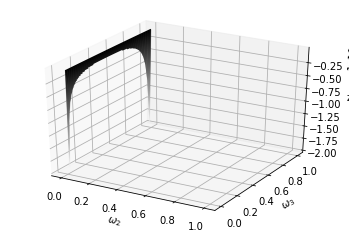
\includegraphics[width=0.49\textwidth]{Chapter4/img/0-01.png}
    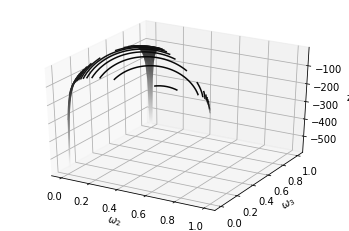
\includegraphics[width=0.49\textwidth]{Chapter4/img/pi-4.png}
    \caption{grid search for different $\alpha$, left: $\alpha=0.01$, right:$\alpha=\pi/4$}
    \label{fig:grid}
\end{figure}

\subsection{A simple first-order method}

Both \XYA~\citep{soare2014linear} and \RAGE~\citep{fiez2019transductive} require to solve an optimization problem of type
\begin{align}\label{eq:fw1}
    \inf_{\bomega\in\Sigma_K} \max_{\bx,\bx'\in\cX} \normm{\bx-\bx'}^2_{\Lambda_{\bomega}^{-1}},
\end{align}
which can be solved by a Frank-Wolfe-typed algorithm applied on the dual problem of~\eqref{eq:fw1} (see e.g.~\citealt{ahipasaoglu2008fw}).

One may notice that the optimization problem that we want to tackle here is of a similar fashion,
\[
    \inf_{\bomega\in\Sigma_K} \max_{\bx,\bx'\in\cX} \frac{\normm{\bx - \bx'}^2_{\Lambda_{\bomega}^{-1}}}{(\bx\transpose\btheta^\star-(\bx')\transpose\btheta^\star)^2}.
\]
It is thus interesting to investigate its dual problem as well. A heuristic is proposed by Degenne et al. (2020) as shown in Algorithm~\ref{alg:solver}, where $\cY$ is defined as \[
    \cY \eqdef \left\{ \frac{(\bx^\star- \bx)}{\left|(\bx^\star-\bx)\transpose\btheta^\star\right|}: \bx\in\cX/\big\{\bx^\star\big\}  \right\}\,.
\]

\begin{algorithm}[ht]
\centering
\caption{Saddle Frank-Wolfe heuristic for computing the optimal weights.}
\label{alg:solver}
\begin{algorithmic}[1]
   \State {\bfseries Input:} arm set $\cX\subset\R^d$, maximum iterations $n$
   \State  {\bfseries Initialize:} $\bomega \leftarrow{} (1, 1, \ldots, 1)\in\R^K, \mathbf{\tLambda} \leftarrow{} I_d, \mathbf{\Lambda}\leftarrow{} I_d, t \leftarrow{} 0$
   \While{$t<n$}
        \State $\mathbf{\tx}\in\argmax_{\bx\in\cX}  \norm{\bx}_{\mathbf{\Lambda}^{-1} \mathbf{\tLambda} \mathbf{\Lambda}^{-1} }^2$
        \State $\mathbf{\ty}\in\argmax_{\by\in\cY}\normm{\by}^2_{\mathbf{\Lambda}^{-1}}$
        \State $\mathbf{\Lambda}\leftarrow{} \mathbf{\Lambda}+ \mathbf{\tx}\mathbf{\tx}\transpose$
		\State $\mathbf{\tLambda} \leftarrow{} \mathbf{\tLambda} + \mathbf{\ty}\mathbf{\ty}\transpose$
        \State $\bomega \leftarrow{} \frac{t}{t+1}\bomega + \frac{1}{t+1}\be_{\mathbf{\tx}}$
        \State $t \leftarrow{} t+1$
   \EndWhile
   \State \Return $\bomega$
\end{algorithmic}
\end{algorithm}

\end{subappendices}
